%% ----------------------------------------------------------------
%% GDP.tex
%% ---------------------------------------------------------------- 
\documentclass[oneside]{ecsgdp}         % Use the GDP Report Style
\graphicspath{{../Figures/}}   % Location of your graphics files
\usepackage[numbers]{natbib}            % Use Natbib style for the refs.
\usepackage{float}				% used to allow exact placement of figures
\usepackage{subfigure}				% used to allow more than one figure on a line
\hypersetup{colorlinks=true}   % Set to false for black/white printing
%% ----------------------------------------------------------------
\begin{document}
\frontmatter
\title      {Unmanned Aircraft Camera Module \\(GDP Group 18)}
\authors{ \href{mailto:ajb2g08@ecs.soton.ac.uk}{Andy Busse},
             \\ \href{mailto:jgac1g08@ecs.soton.ac.uk}{John Charlesworth},
             \\ \href{mailto:mh23g08@ecs.soton.ac.uk}{Michael Hodgson},
             \\ \href{mailto:ps26g08@ecs.soton.ac.uk}{Piyabhum Sornpaisarn},
             \\ \href{mailto:ps6g08@ecs.soton.ac.uk}{Paramithi Svastisinha}
	    }
\date       {\today}
\subject    {ELEC6050 Group Design Project}
\keywords   {GDP 18 Group Design Project Camera Interface Software Hardware JPEG Electronic Engineering}
\supervisor {Dr. Rob Maunder}
\examiner   {Dr. Jeff Reeve}
\degree     {Master of Electronic Engineering}
\maketitle
%% ----------------------------------------------------------------
\begin{abstract}
Given an autopilot module for an unmanned aircraft vehicle (UAV), a camera module was designed, built, and tested to be able to capture still images and transmit them to a ground station through the autopilot module's serial link. The systems described include... (42/200 words so far)
\end{abstract}
%% ----------------------------------------------------------------
\tableofcontents
\listoffigures
\listoftables
\lstlistoflistings
\listofsymbols{ll}{$w$ & weight vector}
\mainmatter


% This is part of the FinalReport document.
% Copyright (C) 2011 Piyabhum Sornpaisarn, Andrew Busse, Michael Hodgson, John Charlesworth, Paramithi Svastisinha
% See the file COPYING in FinalReport/ for copying conditions.

%% ----------------------------------------------------------------
\chapter{Introduction - (ab)}
%% ----------------------------------------------------------------

\section{Description of Problem}

This project seeks to produce a system that is able to interface a camera with an autopilot on board an Unmanned Aerial Vehicle (UAV). The desired module must capture a digital still image from the camera, then transmit this data via a low-bandwidth serial link to the autopilot. The autopilot then re-transmits this data over its wireless (RF) link to a ground station running our customers ground software. Then our customer's software provides a TCP/IP interface, which allows us to capture this data in our own program, and then display the captured image data to the user. Both the Autopilot and our customer's ground station software currently exist.

\begin{figure}[H]
        \centering
        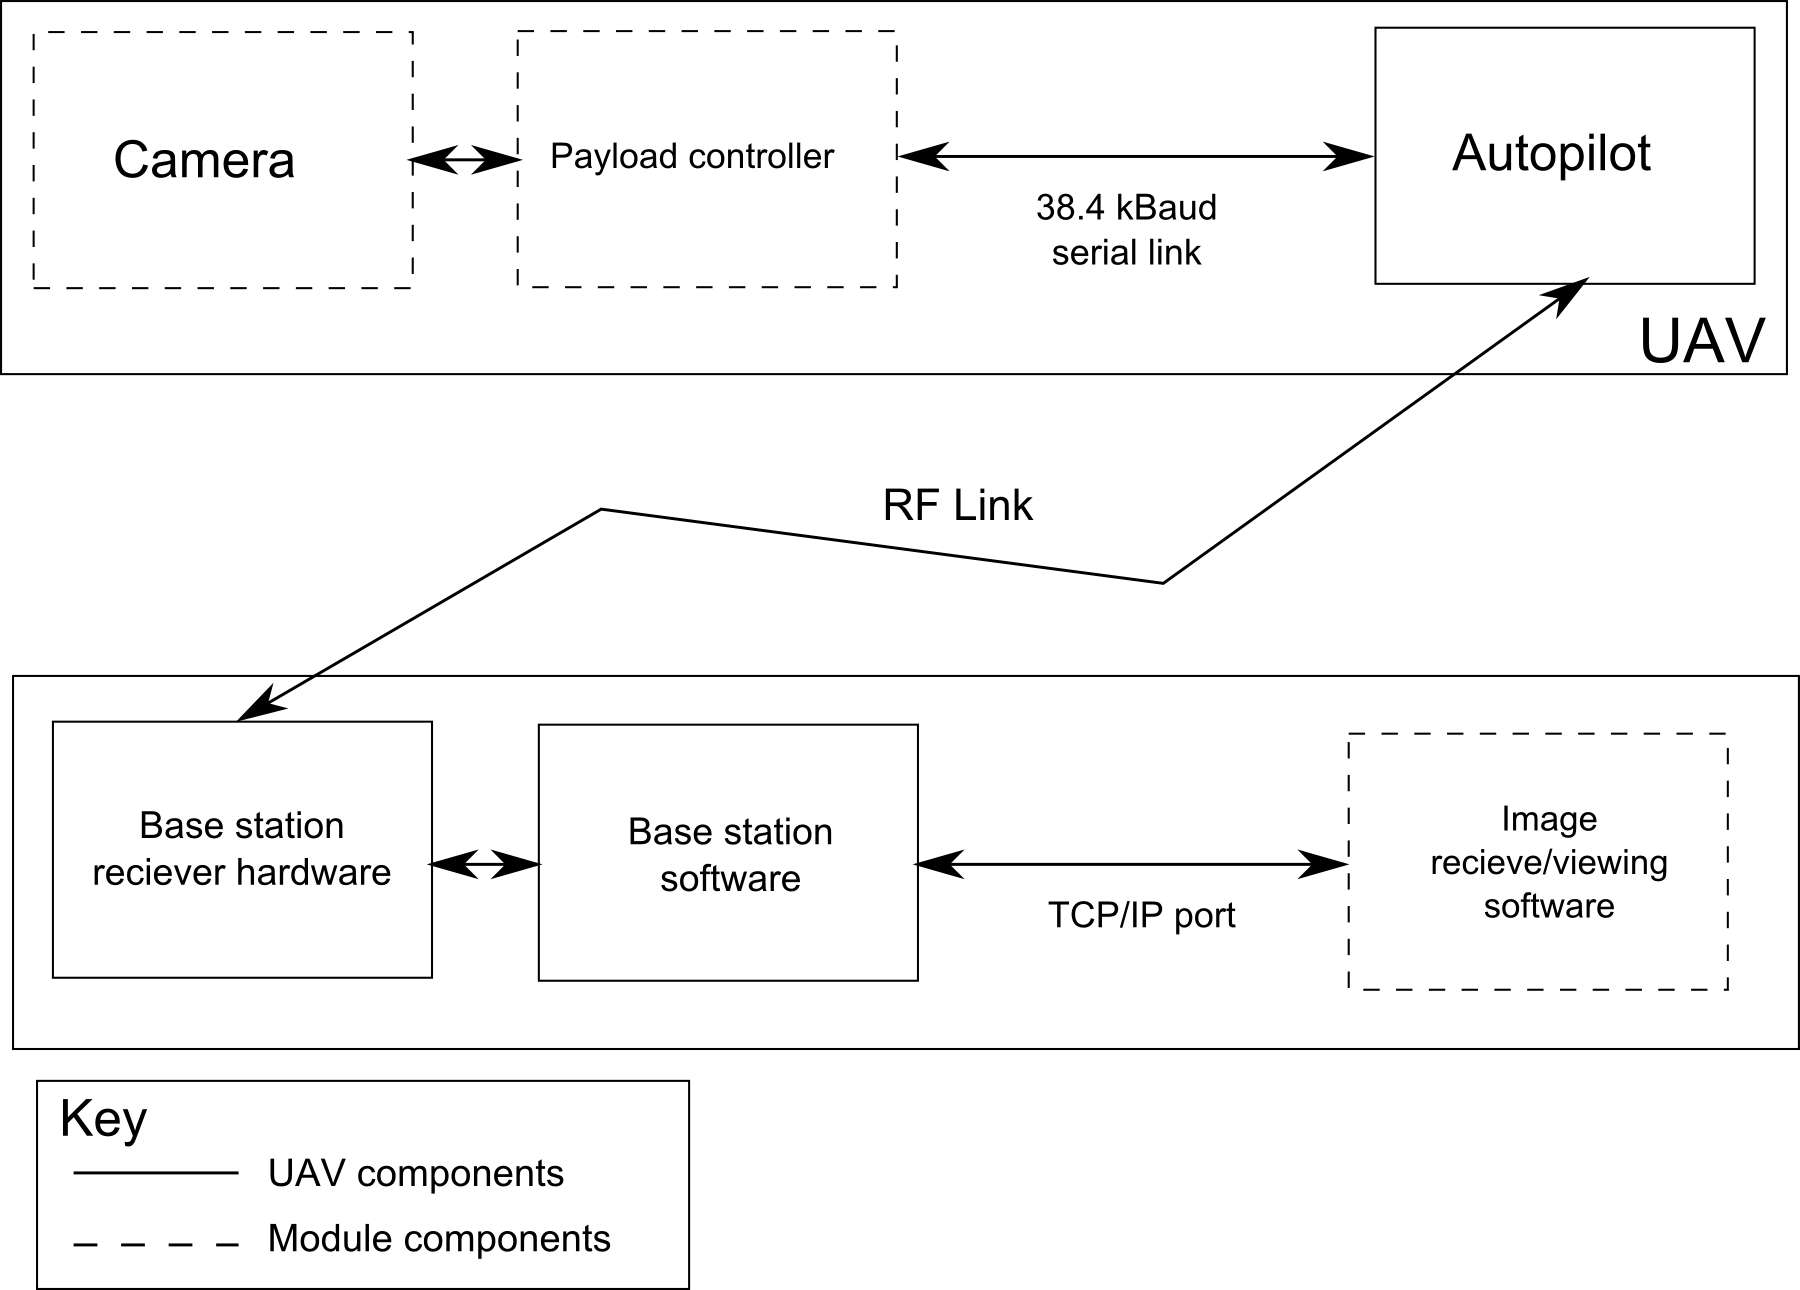
\includegraphics[width=1.00\textwidth]{figures/spec_block_diagram_2.png}
        \captionof{figure}{Block diagram displaying how the separate parts of this project interact, and which parts of this project we need to implement.}
        \label{fig:blockDiagram}
\end{figure}

Deliverables for this project would be a suitable camera for the project, an electronic module presented (preferably) on PCB, and an additional piece of ground station software to interact with the payload module. It needs to be in a state such that it would require minimal additional work before being presented to the clients of our customer as a potential ``Wireless Camera Payload" solution that they would be able to implement. Therefore, delivery of User Documentation, and a repository containing all hardware and software necessary to easily reproduce the project is required.

\subsection{SkyCircuits}

SkyCircuits Ltd. \cite{SkyCircuits} is a company that designs and sells autopilot modules and ground station software for unmanned aircraft. These modules are able to take control of a UAV from take-off to landing, along a user-defined path, with no need for human intervention. SkyCircuits market two different autopilots: A more expensive model aimed at the recreational, academic and commercial markets, and a cheaper, less powerful module, aimed at the Recreational market only.

It was this company's autopilot module that recently successfully flew the world's first 3D-printed UAV, the Southampton University Laser Sintered Aircraft (SULSA), \cite{SULSA} an event which was also covered by the media \cite{SC_Press}.

Our contact from SkyCircuits for this project is its director, Dr. Matt Bennett.

\section{Existing Solutions}
\label{sec:existing_soln}

Currently, SkyCircuits' customers have implemented a system where they have retrofitted a high-resolution camera to a UAV, but this acts entirely independently of the autopilot module, and images are stored locally, therefore there is no way of knowing whether an image taken during flight is any good. The camera used for this system is very expensive (approximately \pounds 2000). The system we present in this project is significantly cheaper than this existing setup.

\section{Project Motivation}

The cost and inflexibility of the existing solution \ref{sec:existing_soln} means that it is unlikely that recreational users will want to replicate this system. Creating a camera payload for the autopilot that is cheaper, more functional (in that it would be able to exploit the wireless link furnished by the autopilot), and open source, is in our customer's interest as it may be useful in furthering interest around their products.

Also, this project serves to test a key piece of functionality of the autopilot modules to its limit - the payload module port. This project serves to test the robustness of this feature, and help iron out any potential bugs, and encourage development of further payload modules. The ability to further develop this project to include other types of payload and further potential applications of the autopilot would potentially increase interest around the products.

Both of the autopilot modules marketed by SkyCircuits Ltd. offer the ``payload" feature.

\section{Solution}

Our solution, presented in Chapter \ref{chap:implementation}, comprises a complete system implemented on PCB, connected to a UAV-mountable board camera, which, when prompted by our software, is able to capture an image, store it locally on an SD card, then send it over the wireless link provided by the autopilot module to a ``ground station" (a laptop configured with the autopilot's wireless receiver and SkyCircuits' software). Our software interacts with the existing software's TCP/IP port, and can send images via the autopilot to the payload, and accept data from the payload and display it on screen.

\section{Report Structure}

Below is a short summary of what each section of this report contains:

\subsection{Background Research}
This section introduces various topics that have been relevant to this project, including:
\begin{itemize}
\item Image Compression Theory
\item JPEG Image Compression 
%\item Automatic Repeat Requests
%\item Parity Bits
%\item ZigBee modules
%\item SkyCircuits Autopilot System
\end{itemize}

\subsection{Specification}
The specification in its submitted form, along with justification for the inclusion of each point.

\subsection{Planning}
Our project plan, including our initial Gantt Chart, Risk Analysis, Skills Audit, Work Allocation, Planned Communication, Resources, Milestones and Technical Plan.

\subsection{Design Choices}
This section explains the various design choices which we have made during this project, including a discussion of the other options that were available to us at the time, and a justification for our choice.

%%...more to follow when report structure is a bit more concrete...

\section{Authorship}

The main author of each section of this report is indicated by initials in 
the title of either the chapter, section, subsection, etc. that the author 
was responsible for writing. Editing the report was the entire group's 
responsibility.

\begin{itemize}
\item ab - Andrew Busse
\item jc - John Charlesworth
\item mh - Micheal Hodgson
\item ms - Paramithi ``Mitch" Svastisinha
\item ps - Piyabhum Sornpaisarn
\end{itemize}

\newpage
%% ----------------------------------------------------------------
\chapter{Background Research}
%% ----------------------------------------------------------------

\section{JPEG Image Compression}
The images obtained from the camera will be in the JPEG image format. If the image data is sent to the ground station progressively, it must be necessary to understand how a JPEG image is structured to reconstruct the encoded image. Unlike raw image data, which can easily be read continuously, JPEG files have already been compressed and contain information which must first be read to properly decompress the image.

\subsection{JPEG structure}
A JPEG file can be separated into two main parts. The first part of the JPEG file is composed of segments containing information concerning various properties of the image which must be read in order to recover the image from its compressed form. The second part contains the entropy-encoded image data, which can be decoded using the information provided from the headers of the file.  

The segments which make up the image file properties are indicated by header markers. ``Each marker is immediately preceded by an all 1 byte (0xff).'' (Header guide) This marker is then followed by a marker identifier byte specific to that segment type. The 0xff value will always indicates the start of the header in this part, but is treated differently in the image data stream. ``If a 0xff byte occurs in the compressed image data either a zero byte (0x00) or a marker identifier follows it.'' (Header guide) 0xff bytes followed by a zero byte are read in as the hexadecimal value 0xff and the 0x00 byte is ignored entirely. 0xff bytes not following this a 0x00 byte are considered to be the header byte of the next segment. If the segment contains useful information before the next marker identifier, it is then followed by two bytes specifying the total length of the segment (in bytes). For the SOS segment, this does not include the entropy-encoded image data.

\subsubsection{JPEG Segments}
The number of headers found within a JPEG image file is not constant between images. The JPEG headers are capable of storing most of the metadata related to an image, not all of which is necessary for the decompression of the image. The following headers are those which contain all the information necessary for a successful decompression of the JPEG image, as well as those which can be found in all JPEG images. The number in brackets next to the segment name is the unique marker identifier value which appears directly after the 0xff marker indicator byte. All numerical values obtained from the byte stream are unsigned. ``DQT, DHT, DRI and SOF may line up in any order, but must be recorded after APP1 (or APP2 if any) and before SOS.'' (Exif)

\paragraph*{SOI: Start Of Image (0xd8)}
This header identifies the start of the image and can be found in all JPEG images. This is the first header to be read in a JPEG file. This header does not contain any information to be stored by the decompression algorithm, but can be useful for differenciating multiple JPEG images from a single data stream.

\paragraph*{APP0: JFIF application segment (0xe0)}
There can be many APP segments in a single image. Subsequent APP segments are named ``APP\emph{n}'' with a marker identifier of 0xe\emph{n} with \emph{n} being the number of the APP segment. This segment does not contain any information necessary to the decompression algorithm used, so all APP segments ignored.

\paragraph*{SOF0: Start Of Frame (0xc0)}
``SOF is a marker code indicating the start of a frame segment and giving various parameters for that frame'' (Header guide) /this indicates that the image is a ``DCT-based JPEG, and specifies the width, height, number of components, and component subsampling (e.g., 4:2:0)'' as well as the data precision (in bits/sample) of an image. (narcap) From the component subsampling information, the size of the Minimum Coded Unit (MCU) which make up the JPEG image. Just like the APP segments, there can be multiple start of frame segments in more complex images, but the images sent by the camera will only need the information contained in the first SOF segment.

\paragraph*{DHT: Define Huffman Table(s) (0xc4)}
This segment defines the properties of one or many Huffman table(s) (HT) which will be used to decode the entropy-encoded image data. ``A single DHT segment may contain multiple HTs, each with its own information byte.'' This segment includes the number of the HT as identified by the image data and the type of the HT (either DC or AC) It also stores the ''number of symbols with codes of length 1..16, the sum (n) of these bytes is the total number of codes, which must be $\leq$ 256'' as well as ``the symbols in order of increasing code length ( n = total number of codes )'' (Header guide). In practice, a single image can also contain multiple DHT segments which all share the same marker identifier. 

\paragraph*{DQT: Define Quantization Table(s) (0xdb)}
This segment defines the properties of one or many quantization table(s).

\paragraph*{SOS: Start Of Scan (0xda)}
This segment gives various scan-related parameters and is the last segment preceding the entropy-encoded image data. This segment associates each component in the scan with the appropriate AC and DC Huffman table by their ID number. 3 ignorable bytes seperate this segment from the image data. 

\paragraph*{EOI: End Of Image (0xd9)}
This header identifies the end of the image. ''It is possible that the end of the image is reached without finding the EOI marker. In this case, the image is technically malformed but the situation is tolerated and handled as if the EOI marker was found.`` (winzip) 

\subsubsection{Entropy-encoded image data}
(Exif)

\subsection{JPEG Header Information Extractor}

\subsection{Progressive Display of Image}

\section{Existing Hardware and Software}
Research concerning the payload and the associated software goes here...

\section{Cameras Available}

%\section{Hardware Selection}
%Research justifying hardware choice goes here...


\newpage
%% ----------------------------------------------------------------
\chapter{Specification}
%% ----------------------------------------------------------------
\label{chap:specification}

\section{Introduction (jc)}

This chapter will describe the brief we were given and an overview of the system and how the elements to be created will sit with the existing components.

The functionality intended for the system is also broken down and the priority given to each task is explained. The things that we should have to give to our customer at the end of the project are also described.

\section{Brief (jc)}

The original agreed project specification and plan, handed in on the first week of the project, was to design, build, and test an electronic module capable of capturing still images from an unmanned aerial vehicle (UAV) and transmitting the images to a ground station. The module must use the UAV autopilot’s low-bandwidth RS485 serial link (38.4 kBaud). A program must be written to interface with the ground station software over a TCP/IP link, allowing commands to be sent to the electronic module in the UAV and image data to be received and then displayed to the user on the ground. The electronic module should be constructed suitably ruggedly for use in the environment of the UAV.

\section{Block Diagram (jc)}

\begin{figure}[H]
        \centering
        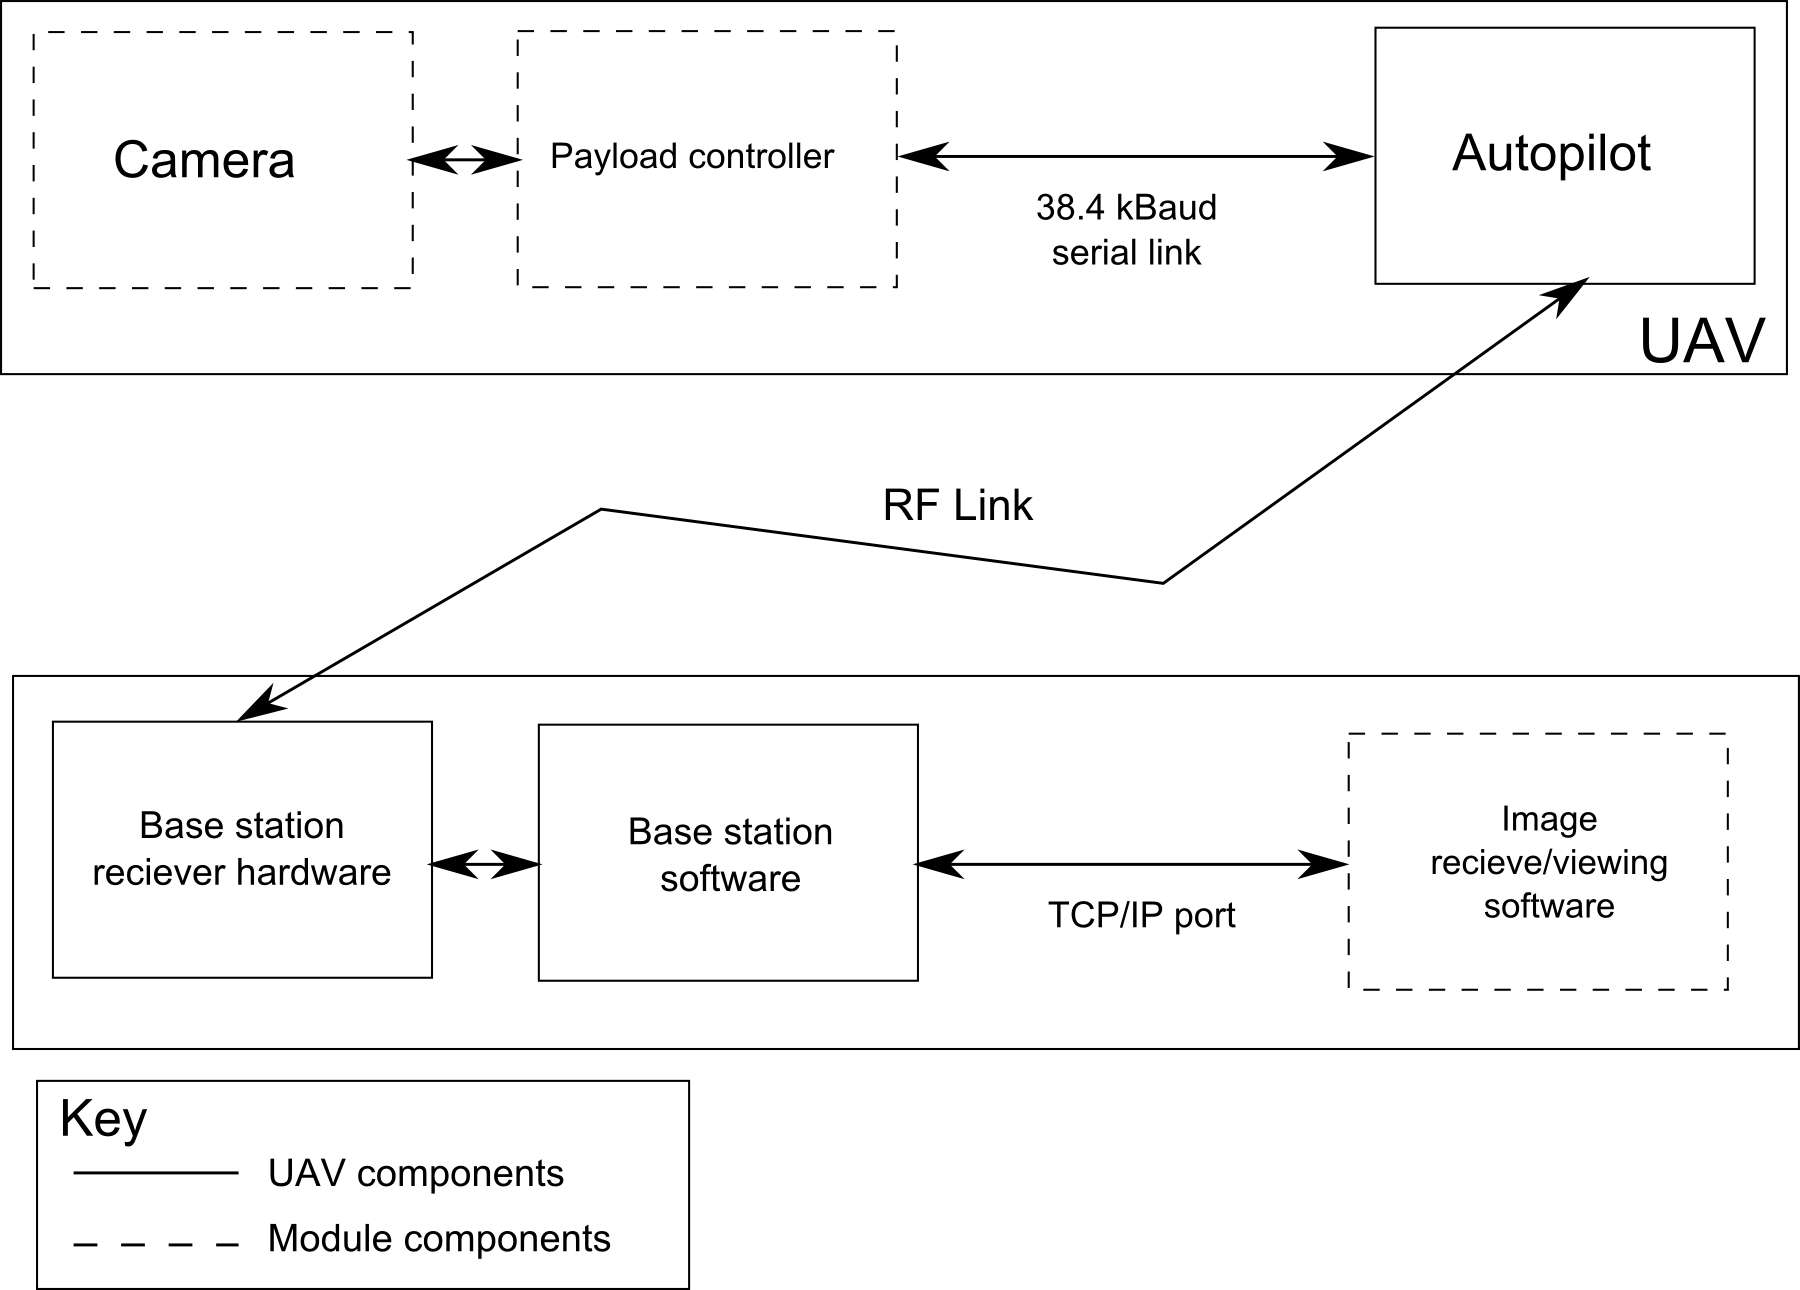
\includegraphics[width=1.00\textwidth]{figures/spec_block_diagram_2.png}
        \captionof{figure}{Block diagram of the specified system}
        \label{fig:block1}
\end{figure}

The above diagram (figure \ref{fig:block1}) gives an overview of how the system described in the specification all comes together. The parts with a solid outline are parts that we were given by our customer to fit our system around. The parts with the dashed outline are the elements of the design that we need to implement ourselves.

Inside the UAV itself will go the camera, the payload controller and the autopilot. The autopilot is provided by our customer and also provides our wireless link to the ground. The camera is simply a camera so that photographs can be taken. The payload controller is the part that needs the most work, it needs to be able to control the camera; take and get images as well as being able to communicate with the autopilot and interpret any commands sent up from the base station (also referred to as the ground station).

On the ground station side of things there is a radio frequency (RF) link to the autopilot (simulated by a USB cable for development purposes) which attaches to a computer running the ground station software provided by our customer. The ground station software provides two TCP/IP ports as interfaces, one for sending commands to the ground station software and to the autopilot and one for streaming data from the autopilot. It is these TCP/IP ports that our software on the ground has to interface with so that it can send commands up to the payload controller and then receive and display an image.

\section{Objectives (jc)} 

The aim of the project was to achieve the following criteria, which were also prioritized in order to ensure organized and efficient work - high priority points are essential or very important to basic system functionality, medium priority points are not essential for basic functionality but help expand the system into a more complete system and low priority points are optional extras that should be added if time permits or if they are very low effort:

	\subsection{Specification A}\label{sec:spec_a} \textbf{The image should be encoded in such a way that a low quality image will be available quickly, the quality of which would improve as more information is downloaded.} This was given a \textbf{high priority} as raw images of an acceptable resolution (see below) contain a large amount of data and we have a slow communications link therefore it would be extremely beneficial to be able to view a low quality image quickly so that you don't have to wait for the full image download to judge its appropriateness.
	\subsection{Specification B}\label{sec:spec_b} \textbf{Minimise the time needed to download the images from the UAV to the base station. The time from the user’s prompt until the image has been fully downloaded will be measured against the theoretical 3 minutes necessary to transmit a full image without using any compression. The goal will be to obtain a full image in \textbf{less than 3 minutes.}} 
This 3 minute figure is the time it was calculated it would take to download a raw $640\times480$ 24bit RGB image (approx. 900kB) at 38.4kBaud. This was given a \textbf{high priority} as 3 minutes is a long time to wait for an image to download and downloading images is the point of our system.
	\subsection{Specification C}\label{sec:spec_c} \textbf{The module weight will be \textbf{less than 250g}.} 
This was given a \textbf{medium priority} since although a weight of under 250g would be required for flight, it would be preferable to have a system that is too heavy than one that does not work at all.%as electronics tend not to be very heavy but it is important to bear in mind that the UAV can't carry too much weight.
	\subsection{Specification D}\label{sec:spec_d} \textbf{Image resolution of at least \textbf{$640\times480$}.} 
This was given a \textbf{medium priority}, this value was chosen as a trade off between the amount of data in the image and the quality of the image. Higher resolutions would be acceptable if the download time can be suitably reduced and lower resolutions may also be useful if they are much faster to download.
	\subsection{UAV Camera Commands} \textbf{Allow the user to perform the following actions on the UAV’s camera from the ground station:} 
		\subsubsection{Specification E}\label{sec:spec_e} \textbf{Prompt the UAV to \textbf{capture and download an image}.}  
This was given a \textbf{high priority} as the main aim of the system is to be able to capture images.
		\subsubsection{Specification F}\label{sec:spec_f} \textbf{\textbf{Cancel} the downloading of any image while the image is being downloaded.} 
This was given a \textbf{medium priority} because, given the potentially high download times, a lot of time could be saved by being able to cancel the download of an image you do not want before it has fully downloaded but it is not essential to the basic functionality of the system.
		\subsubsection{Specification G}\label{sec:spec_g} \textbf{\textbf{Resend} an image in case the current preview is corrupted.}  
This was given a \textbf{low priority} as it does not affect basic functionality.
		\subsubsection{Specification H}\label{sec:spec_h} \textbf{\textbf{Interrupt} the download of an incomplete image and allow the user to save the incomplete image.}  
Please note that this is distinct from the \emph{Cancel} (\ref{sec:spec_f}) requirement mentioned above since it requires the saving of incomplete images. This was given a \textbf{low priority} as it does not affect basic functionality, but could potentially save the user some time.
		\subsubsection{Specification I}\label{sec:spec_i} \textbf{Select the \textbf{resolution settings} of the image.}  
This was given a \textbf{low priority} as it does not affect basic functionality but could be a useful feature for some users.
		\subsubsection{Specification J}\label{sec:spec_j} \textbf{Display a progress indicator which will show the percentage of the image data received, as well as a time estimate for the rest of the image to be downloaded.} 
This was given a \textbf{low priority} as it does not affect basic functionality but allows the user to feel more confident that the system is working.
		\subsubsection{Specification K}\label{sec:spec_k} \textbf{The image capture will be triggered automatically by the UAV using triggers built into the autopilot.}  
This was given a \textbf{low priority} as it does not affect basic functionality but could be something a user might like to be able to do.
		\subsubsection{Specification L}\label{sec:spec_l} \textbf{Allow the user to command the image capture to \textbf{trigger periodically} over a \textbf{user specified time interval} will be added if time permits.} 
This was given a \textbf{low priority} as it does not affect basic functionality but may be a useful feature for some users.
	\subsubsection{Specification M}\label{sec:spec_m} \textbf{Images will be transmitted in \textbf{colour} as opposed to black and white.}  
This was given a \textbf{low priority} as black and white images are still useful but colour images would be preferred.
	\subsubsection{Specification N}\label{sec:spec_n} \textbf{The user should be able to select between a colour image and a black and white image.}  
This was given a \textbf{low priority} as it does not affect basic functionality.


\section{Deliverables - (ms)}

The deliverables which were planned to be produced by the end of the project and given to the customer include:

	\subsection{\underline{Hardware}:} 
	\label{sec:deliv_hw} 
	Camera module, constructed on PCB (if time permits, otherwise on strip-board), including layout designs.
	\subsection{\underline{Software}:} 
	\label{sec:deliv_sw} 
	All firmware for the electronic module, and software on the base station for viewing images. The full source code and all executable files will be included.
	\subsection{\underline{Documentation}:} 
	\label{sec:deliv_doc} 
	Technical and User Documentation. This includes all schematics related to hardware as well as all other documents concerning both the software and hardware delivered.
	\subsection{\underline{Public repository}:} 
	\label{sec:deliv_git} 
	The full source code, all schematics, and all documents concerning both the software and hardware will be included on a public repository so that the customer may share this information with his clients.


\newpage
%% ----------------------------------------------------------------
\chapter{Design Approaches Considered}
%% ----------------------------------------------------------------

\section{Payload Image Capture}

\subsection{Camera Module}
John

\subsubsection{Approach: Analogue Camera}	
Short description of the approach
Advantages:
\begin{itemize}
\item Blah
\item Blah
\end{itemize}

Disadvantages:
\begin{itemize}
\item Blah
\item Blah
\end{itemize}

Conclusion of approach


\subsubsection{Approach: Serial Camera}

\subsubsection{Approach: USB Camera}


\subsection{Image Buffering}
Andy.


\subsubsection{Approach: Flash Chip}

\subsubsection{Approach: SD Card}

\subsubsection{Approach: SRAM}
Or whatever it is called


\section{Payload Controller Hardware}
The hardware used to implement the payload controller is an important consideration.

The exact requirements for this module depend on other design decisions made, such as the method used to interface with the camera module. However there are a certain fixed set of requirements derived from the specification:

\begin{itemize}
\item The module must communicate with the autopilot over an asynchronous RS-485 serial connection at 38.4 kBaud. This suggests that the module should have access to some form of UART.
\end{itemize}

Additional requirements depend on other design decisions:

\begin{itemize}
\item \emph{Camera communication:} Using a serial camera would mean the controller requiring access to another UART, while using a USB camera leaves the camera needing access to a USB host interface. Similarly using an analogue camera would mean either the controller be capable of digitising the camera data itself or having a method of interfacing with an external digitiser.
 
\item \emph{Image buffering:} Most embedded systems do not have enough RAM or Flash to store a reasonable sized image on onboard memory. As described in section \ref{sec:local_storage}, there are a number of approaches worth considering for externally buffering an input image, however these do require the controller to have an interface with which to communicate with the external memory. 

\item \emph{Progressive JPEG Manipulation:} Section \ref{sec:implementation_progressive_jpeg} details several ways progressive JPEG manipulation could be tackled. Depending on the design choice taken this could influence the requirements of the controller substantially. Examples of such requirements could be: extra processing power, fast access to memory or FFT or DCT libraries being available for the device.
\end{itemize}

\subsection{Approach: Digital Signal Processor (DSP) Development Board}
An appropriate Digital Signal Processor (DSP) development board would provide fast digital signal processing capabilities to the controller. This would be especially useful for the situations mentioned in section \ref{sec:implementation_progressive_jpeg}.

Since DSP chips tend to be specialist devices they are usually difficult to set up or program without first experimenting with the design using a development board - a special board designed with experimentation and product development in mind. Ideally a development board would be used for initial development of the system with a integrated PCB being developed later on to allow the DSP to be used on its own.

Advantages:
\begin{itemize}
\item DSPs often have very good analogue to digital conversion built in as standard. If an analogue camera is used (as discussed in section \ref{sec:Analog_option}) a DSP may provide the necessary fast ADC without any extra components.

\item Libraries for tasks such Fast Fourier Transforms or other signal and image processing related applications are often readily available for DSP chips. For some methods of performing progressive JPEG manipulation (see section \ref{sec:implementation_progressive_jpeg}) this could be useful.

\item Large number of miscellaneous signal processing related hardware features built in which could be useful in as-yet unforeseen circumstances.
\end{itemize}

Disadvantages:
\begin{itemize}
\item DSP chips are often complex and may require significant work to produce a system running without a development board.

\item DSP development boards often cannot be used effectively in a final version of a project due to size and power constraints.

\item There is a steep learning curve to using these devices and the group has very little experience with them.
\end{itemize}


DSP boards are a specialist tool, which could be especially useful - if not required - if implementing certain image processing algorithms such as some of those detailed in section  \ref{sec:implementation_progressive_jpeg}|. The downside of this is a more complex overall system.

\subsection{Approach: Atmel 8-bit AVR}
\label{sec:desappr:avr}
The Atmel 8-bit AVR family is a well-known set of low cost, single chip microcontrollers. Specific parameters taken from \cite{megaAVR_parameters}.

Advantages:
\begin{itemize}
\item All members of our group have had experience working with AVR chips.

\item Programming and debugging devices are readily available to us.

\item Creating stand-alone systems easy: no need for large amounts of additional components.

\item Commonly used devices mean large community built around the device family meaning support and additional libraries are more likely to be available.

\item Some initial payload code available to us already implemented on a AVR, see section \ref{sec:team_resources}.

\item Large range of different devices which work with the same programming tools and minimal code changes available.

\item Many through-hole versions of the devices are available, making prototyping significantly easier (and cheaper, due to lack of need for breakout boards) than using surface mount components.
\end{itemize}

Disadvantages:
\begin{itemize}
\item Most 8-bit AVR devices are reasonably low speed (20MHz maximum), meaning they could be unsuitable for heavy calculations such as image processing.

\item 8-bit AVRs do not have floating point processing units, making some image processing tasks much slower to complete on an AVR.

\item Less communication options than some other, more complex, devices. This limits the number of peripheral devices that can be connected to the controller at once, and so may reduce flexibility.

\item Limited RAM available on the commonly used devices which are available in through-hole format. A common amount of RAM for a larger through-hole AVR is 4 kbytes.

\item The smaller, cheaper, devices have reasonably limited program memory, with 64 kbytes being a typical amount for a larger through-hole device. This could be a problem if implementing large amounts of code or using significant numbers of lookup tables for example.
\end{itemize}
	
AVRs are robust, widely used, general purpose microcontrollers. The large community surrounding them is a particular advantage, as it means many libraries and development boards are available for the devices. Our previous experience with the devices is also a key advantage, although it is important to be aware of the devices limits.


\subsection{Approach: Atmel 8-bit AVR with Arduino Prototyping Platform}
\label{sec:appr_considered_arduino}

The Arduino platform is a low cost, open-source development platform for the Atmel AVR microcontroller family. The latest versions of the development platform consists of an ATMega328 microcontroller along with voltage regulators, inbuilt USB programmer and serial interface and 16MHz crystal. A software library for the device provides a wrapper around many of the complexities of the AVR platform, allowing more rapid development to be possible than with a pure AVR. A simple IDE is used to program the device and a wide range of extra libraries are available which target the platform. The physical platform is designed to be easily extended using expansion boards called `shields'.

The advantages and disadvantages of the Atmel 8-bit AVRs mentioned in section \ref{sec:desappr:avr} also apply.

Advantages:
\begin{itemize}
\item Just an ATMega328 `under the hood' meaning that the additional power of the chip can be leveraged if needed.

\item Many common tasks such as setting the baud rate of the serial link are made very simple by the Arduino libraries, meaning development time can be spent working on more challenging features.

\item Very widely used by hobbyists, meaning a large number of open-source libraries are available for the platform.

\item Platform is easily available meaning others should more easily be able to replicate project. Widely used platform means plenty of support is available for others wishing to re-implement this project.

\item Since only a `shield' expansion board would need to be manufactured this would cut time otherwise spent designing and making board for AVR.
\end{itemize}

Disadvantages:
\begin{itemize}
\item Using the Arduino libraries means a certain amount of unused overhead is likely.

\item The Arduino libraries hide much of the complexity of the device. This can mean advanced features are hidden or not exposed, negating some of the advantages of the library when advanced features are needed.

\item Design would consist of two parts: Arduino board and expansion `shield'. This could reduce durability and increase size.
\end{itemize}

Using an Arduino has the advantage of speeding up development at the beginning of the project. The large number of libraries built for the Arduino is another key advantage, as is the ease of re-implementation.

\subsection{Approach Chosen}
We chose to use an Atmel 8-bit AVR as the platform for our implementation of the payload controller. Our main reason for choosing this platform is because we already have experience in using this microcontroller, meaning less time to develop and 
test the system over a DSP based solution. Another key reason was the ease of implementing AVR based systems as 
stand-alone boards.

\section{Communication between Payload Controller and Ground Station}
One of the key tasks of the payload controller is to communicate with the Ground Station via the Autopilots 38.4 kBaud serial link. In order to fulfil the specification the payload controller must be capable of receiving messages/commands sent from the Ground Station image viewer software (see section \ref{chap:implementation_ground_station}) through the autopilot link, as well as be capable of sending data to the Ground Station Image Viewer.

The autopilot provides a number of ways to communicate between a payload module and ground station software. The Ground Station software provided to us allows a `packet' of data to be sent to a payload module by executing the command shown below

Another method of communication is via the use of shared memory. Each registered payload module is assigned a set of shared memory which can be read and set by the payload module and the ground station software. This could be used to implement two-way communications between the two subsystems.

The design approaches taken regarding this communication from the perspective of the Ground Station Image Viewer software is discussed in section \ref{chap:implementation_ground_station}.

\subsection{Approach: Shared Memory for Both Directions}
One possible way of producing two-way communications would involve two sets of shared memory: one for ground station to payload messages and another for payload to ground station messages. Both the payload and the autopilot would need to poll the shared memory to check for new messages.

%Advantages:
%\begin{itemize}
%\item 
%\end{itemize}

Disadvantages:
\begin{itemize}
\item The payload must access shared memory by sending a command to request a copy of its contents to be sent via the payload-autopilot serial link. This extra overhead would slow down communications.
\end{itemize}


\subsection{Approach: Send Bytes Command and Shared Memory}
The send bytes command could be used to send messages from the Ground Station to the payload, with shared memory being set by the payload to send messages back from the payload to the Ground Station.

Advantages:
\begin{itemize}
\item No overhead needed to get messages on the payload, they are sent directly from the autopilot to the payload, no polling needed.
\end{itemize}

%Disadvantages:
%\begin{itemize}
%\item Error coding??
%\end{itemize}

\subsection{Approach Chosen: Send Bytes Command and Shared Memory}
Using shared memory for one direction and send bytes for the other seemed like a sensible choice due to the lower overhead needed.



\section{Ground Station Image Viewer}
Peak

\section{Progressive JPEG Manipulation}
Mitch

\section{Physical Implementation}
Andy
	
\subsection{Power Source}

\subsubsection{Approach: Battery Powered}

\subsubsection{Approach: Autopilot Powered}


\newpage
%% ----------------------------------------------------------------
\chapter{Chosen Design Approaches}
%% ----------------------------------------------------------------


\section{Camera module}
\label{sec:John_chosen_options}

The camera type chosen was a serial camera as described in \ref{sec:Serial_option}. The particular model chosen was uCam (microCam) or the "Camera Module - Serial JPEG TTL" from the "coolcomponents" website.

The feature set of the uCam is as follows:
	\begin{itemize}
		\item It can output images in both RAW and jpeg formats
		\item It can output RAW images at a range of resolutions:
		\begin{itemize}
			\item 80 x 60
			\item 160 x 120
			\item 320 x 240
			\item 640 x 480
			\item 128 x 128
			\item 128 x 96
		\end{itemize}
		\item It can output jpeg images at a range of resolutions:
		\begin{itemize}
			\item 80 x 64
			\item 160 x 128
			\item 320 x 240
			\item 640 x 480
		\end{itemize}
		\item it can output RAW images with a range of colour settings:
		\begin{itemize}
			\item 2bit Gray Scale
			\item 4bit Gray Scale
			\item 8bit Gray Scale
			\item 8bit Colour
			\item 12bit Colour
			\item 16bit Colour
		\end{itemize}
		\item It will auto-detect baud rates from 14400 to 115200
		\item It has selectable baud rates up to 1228800
		\item Small physical size at 32mm x 32mm
		\item Well documented
	\end{itemize}

The camera was chosen because this feature set meets the specification and also allows for additional functionality, such as setting the resolution, if the full feature set is exploited.

\section{Payload/Ground Station Interaction}

\section{Ground Station Image Viewer}

\section{Progressive JPEG Manipulation}

\section{Physical Implementation}

The final, delivered module is a $90mm\times62mm$ PCB. The PCB manufactured 
for the project was done so for free, using Spirit Circuits' "Go Naked"
service \cite{go-naked}. The PCB itself is a "tracks and holes" only service 
- no soldermask or silkscreen is applied. The schematic of the circuit 
delivered is available in Appendix ???, and of the PCB layout in Appendix 
???. A waterproof lacquer will be applied to the PCB to prevent condensation 
from shorting tracks together, and the module itself presented in a 
waterproof container before flight testing.

\begin{figure}[H]
        \centering
        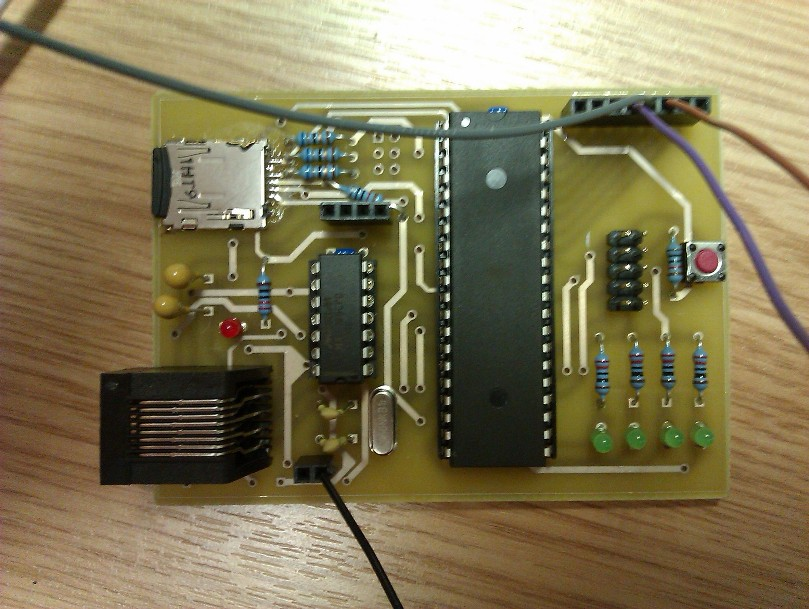
\includegraphics[width=1.00\textwidth]{figures/PayloadImplementation.jpg}
        \captionof{figure}{Image of the final payload, under test, before lacquer is applied. R11 can be seen between the Camera header and a via near the SD card Vcc}
        \label{fig:PayloadImplementation}
\end{figure}

Due to an issue discovered between ordering and receiving the PCB, an 
additional 10k$\Omega$ resistor has been placed between Camera RX and 3V3 (R11 
on the schematic). Also, the Single In Line header holes (for the Port A 
expansion and camera headers) have been widened from 0.40mm to 0.80mm. An 
update to the PCB layout is provided in the delivered repository.

The camera will also be presented in a sealed, weatherproof container.

\section{System Design Overview}


\newpage
%% ----------------------------------------------------------------
\chapter{Implementation - Payload}
%% ----------------------------------------------------------------
\label{chap:implementation}

\section{Overview (mh)}

The payload controller module is an important part of the system, responsible
for interfacing with the camera module and communicating with the ground 
station image viewer software via the autopilot. Since this single module 
encapsulates a significant amount of the complexity of the project it was 
deemed sensible to split it up into sub-modules, which could be worked on in
parallel by different members of the team. 

With this in mind the payload controller module was split into four main 
submodules:

\begin{itemize}
	\item Camera Module Communication
	\item Communication with Ground Station via Autopilot
	\item SD Card Image Buffering
	\item Progressive JPEG Manipulation
\end{itemize}

%||||||| INCLUDE REFERENCES TO EACH ||||||||||

%||||||| INCLUDE SUBMODULE DIAGRAM OF THE PAYLOAD MODULE |||||||

\subsection{Camera Module}
\label{sec:John_Implementation}

The first step in the implementation of the camera module was to verify the communication with the camera by talking to it via a pc. Once this step was complete the next step was to implement communications between the camera and a microprocessor, with the pc for debugging. With the microcontroller able to communicate with the camera this module was ready for integration with the payload.

\subsubsection{First camera}


\section{Interfacing the Arduino with an SD card (ab)}
\label{sec:SD_imp}

Interfacing the arduino with an SD card is made possible using the arduino SD card library \cite{arduino_sd_library}. Using an Arduino Uno,
 a multiple-size SD card socket from Zepler stores, and the 
"ReadWrite" test program provided in the arduino-022 IDE, we connected the following Arduino pins to the following SD card pins:

\begin{itemize}
\item Arduino GND - SD GND (pins 3 and 6)
\item Arduino 3V3 - SD Vdd (pin 4)
\item Arduino Digital pin 11 - SD MOSI (pin 2)
\item Arduino Digital pin 12 - SD MISO (pin 7)
\item Arduino Digital pin 13 - SD SCLK (pin 5)
\item Arduino Digital pin 4 - SD CS (pin 1)
\end{itemize}

Communication with the SD card only works in SPI mode, unfortunately the built-in 
SD card library does not support 1-wire or 4-wire SD mode.

\subsection{File Naming System}

This example program is useful, but only allows us to write to one file name at 
a time. Therefore, a method was written, see appendix \ref{lst:arduino_captureTest}, lines 62-68 that detects all of files present on the SD card, increments the filename, and 
writes the new data to that filename.


\section{Communication with Ground Station via Autopilot (mh)}
\label{sec:payload controller}
Considering the overall aim of this project: to produce a system by which 
images can be downloaded over-the-air from a payload module to a ground 
station, some method of communicating between the
payload module and ground station are an essential component in the system.

The specification requires the payload
module to communicate with the ground station using the autopilots payload
module interface (discussed in section \ref{sec:autopilot_payload_interface}).

%To better explain the protocol used we will split the explanation into two 
%sections: a \emph{Autopilot Payload Interface} section describing the
%pre-existing autopilot payload interface on which we are building the 
%protocol and a \emph{UAV Camera Communication Protocol} section describing the 
%protocol we have implemented as a part of this project.

\subsection{Existing Code}
\label{sec:payload_existing_code}
Our customer had provided us with some payload module communication AVR code
- written for a ATMega168 - for communicating with the autopilot. This code
was the basis on which the payload controllers communication link was built.

The code provided a number of useful utilities:
\begin{itemize}
\item Basic connection to the autopilot, including responding to transmit tokens.

\item Ability to set shared memory on the autopilot.

\item Ability to receive messages sent from the Ground Station to the 
autopilot.

\item Example code for setting shared memory on the autopilot.
\end{itemize}

This base code was modified slightly after a bug was found in its handling of 
the transmit enable signal. The RS485 communication protocol used for the 
autopilot-payload link (as described in section |||||||| SEC ||||||||) 
requires a `transmit enable' signal to be asserted when the payload is 
transmitting. This signal should be asserted just before data is to be sent 
and cleared just after. However, the original payload base code cleared this 
signal in an interrupt service routine (ISR) which fired after the transmit 
buffer of the UART was ready to accept new data. Since this transmit buffer 
would be ready to accept new data before the data was actually sent over the
physical connection this lead to the transmit enable signal being cleared
before all data had been sent, causing strange behaviour on the RS485 link.
This bug did not seem to cause any problems, and the odd behaviour was only
noticed when testing the system with an oscilloscope. ||||| INC TRACES ||||||
It was considered sensible to fix the bug in case it did cause problems later.

The fix for this problem was reasonably simple: a new ISR was set up which 
fired only when the current transmission had actually completed, and the 
command to clear the transmit enable signal was moved into this ISR.
||||| INC AFTER TRACE ||||||

\subsection{Establishing Contact with the Autopilot (mh)}

The first step in implementing the communications link was to establish contact with
the autopilot using the existing module code, the relevant milestone being
\ref{sec:ms_pl_tx_token_resp}. 

A problem was encountered during this step where the payload would not 
respond to a transmit token in any way. Debugging this problem with a 
oscilloscope showed that the autopilot was not sending transmit tokens.

After spending some time ruling out problems with our own design that could be
causing this, including looking at the RS485 chip in case it was conflicting with the
autopilots serial bus or malfunctioning, we contacted our customer and queried 
whether it could be a problem with the autopilot itself, presenting our evidence of
debugging.

Our customer responded by acknowledging that it was a problem with the autopilot
and providing us with an updated firmware for the autopilot
which would send the transmit tokens correctly.

After this bug was fixed the payload responded as expected, 
section \ref{sec:test_pl_est_contact} describes the successful testing of this part of
the implementation.

\subsection{Setting Shared Memory on the Autopilot (mh)}
Once basic contact had been established the next task was to set shared memory on
the autopilot - as per milestone \ref{sec:ms_pl_shared_mem_set}. The existing code
provided allowed this to be completed quickly using the built in functions. Section 
\ref{sec:test_pl_set_shared_mem} details the tests carried out to validate this
was working.

\subsection{Recieving Messages from the Ground Station (mh)}
It was important to ensure that the payload recieved messages correctly from the ground
station before continuting with the implementation of this section, the customers provided code
allowed this to be completed quickly also. Section \ref{sec:test_pl_receive_message} describes 
the steps taken to test this.

\subsection{UAV Camera Communication Protocol (mh)}
As discussed in section |||||||| REF |||||||| it was decided that 
our communications protocol would use shared memory and \emph{send\_bytes} 
commands, allowing two way communications between the payload controller and 
ground station software to be established. With the ability to receive and send data
with these messages tested as described above, implementation could now begin on
implementing a communications protocol used to talk between the our ground station 
image viewer software and the payload.

The method through which this shared memory is accessed via the ground station
image viewer is discussed in chapter \ref{chap:implementation_ground_station}.

%The Payload Module Interface discussed above (section \ref{sec:autopilot_payload_interface})
%allows us to send strings of bytes in both directions. However, in order to 
%communicate with the ground station image viewing software some form of 
%additional communications protocol is required so that both ends of the link 
%are communicating in a mutually understandable manner.

This two way communications is the interface between the payload and the 
ground station software, so some standard protocol was required. It was decided
that a message based system would be used, with the messages from the ground
station to the payload module being sent using \emph{send\_bytes} and the 
messages sent from the payload to the ground station being put into shared
memory. Each message is composed of two elements, one byte for the message ID 
- unique to each type of message - and a variable number of data bytes 
(depending on the message type.) The different message types are detailed 
below:

\subsubsection*{Messages sent from Ground Station To Payload}

\begin{itemize}
\item \textbf{Take Picture}
\begin{itemize}
\item \emph{Data:} None
\item Prompts payload module to capture an image and save it to the SD card.
\end{itemize}

\item \textbf{Image Download Request} 
\begin{itemize}

\item \emph{Data:} Image ID
\item Requests the payload send the image with ID \emph{Image ID} to the 
ground station. This message allows any image stored by the payload module 
to be downloaded over the connection, increasing flexibility. 
\end{itemize}

\item \textbf{Configure Camera}
\begin{itemize}
\item \emph{Data:} Colour Type, Raw Image Resolution, JPEG Image
Resolution
\item Sets the image resolution and colour mode of the camera. Only the 
JPEG mode has been tested so far.
\end{itemize}

\item \textbf{Cancel Download}
\begin{itemize}
\item \emph{Data:} None
Resolution
\item Cancels the current download taking place.
\end{itemize}

\end{itemize}

\subsubsection*{Messages Sent from Payload to Ground Station}

\begin{itemize}

\item \textbf{Picture Taken}

\begin{itemize}
\item \emph{Data:} Image ID

\item Informs the ground station software that an image has been taken and 
saved to the SD card. \emph{Image ID} is the ID of the image that has been 
saved to the SD card.
\end{itemize} 

\item \textbf{Image Download Info}

\begin{itemize}

\item \emph{Data:} Number of Image Packets

\item Sent by the payload after a successful \emph{Image Download Request}
message from the ground station. Informs the ground station how many 
\emph{Image Data} packets to expect.
\end{itemize}

\item \textbf{Image Data} 
\begin{itemize}
\item \emph{Data:} Packet Number, Image Data
\item This message contains an amount of actual image data. Sent after a
\emph{Image Download Info} message which is in turn in response to an 
\emph{Image Download Request} message. The whole image is sent over
\emph{Number of Image Packets} packets (as defined by the \emph{Image Download
Info} message.) \emph{Packet Number} informs the ground station which of these
packets the message is carrying. \emph{Image Data} contains the actual image 
data for this packet and is variable size, with a maximum size of 50 bytes. 
\end{itemize}

\end{itemize}

Implementing this communications protocol was a significant challenge and was a major
component of the payload module implementation. 

Our implementation for the payload follows an event loop style, where an initial series of 
steps are preformed initializing the camera and SD card, after which the code then enters a continuously
running loop which checks to see if any messages have been received from the ground station.

When a message is received from the ground station (as sent by \verb+send_bytes+ command) a switch-case
conditional structure then decodes which message had been sent and
initiates the appropriate function on the payload (for example calling the camera code to take a picture when sent
a \emph{Take Picture} command).

%One problem encountered during the implementation was that when attempting to set shared
%memory using the payload module, the send buffer implemented in the customer's existing code
%could fill up


The basic sequence for sending data from the payload controller to the autopilot is to use the utilities provided 
by the customers existing code to place messages into the autopilots shared memory to be accessed by the
ground station, as described earlier. Only one set of shared memory is used, and is overwritten every time 
a new message is to be sent from the payload controller to the ground station.
Other features such as configuration of camera resolution are implemented using this basic mechanism, figure \ref{sequence diagram} describes many the sequence diagram of the data transmission.


\begin{figure}[H]
\begin{center}
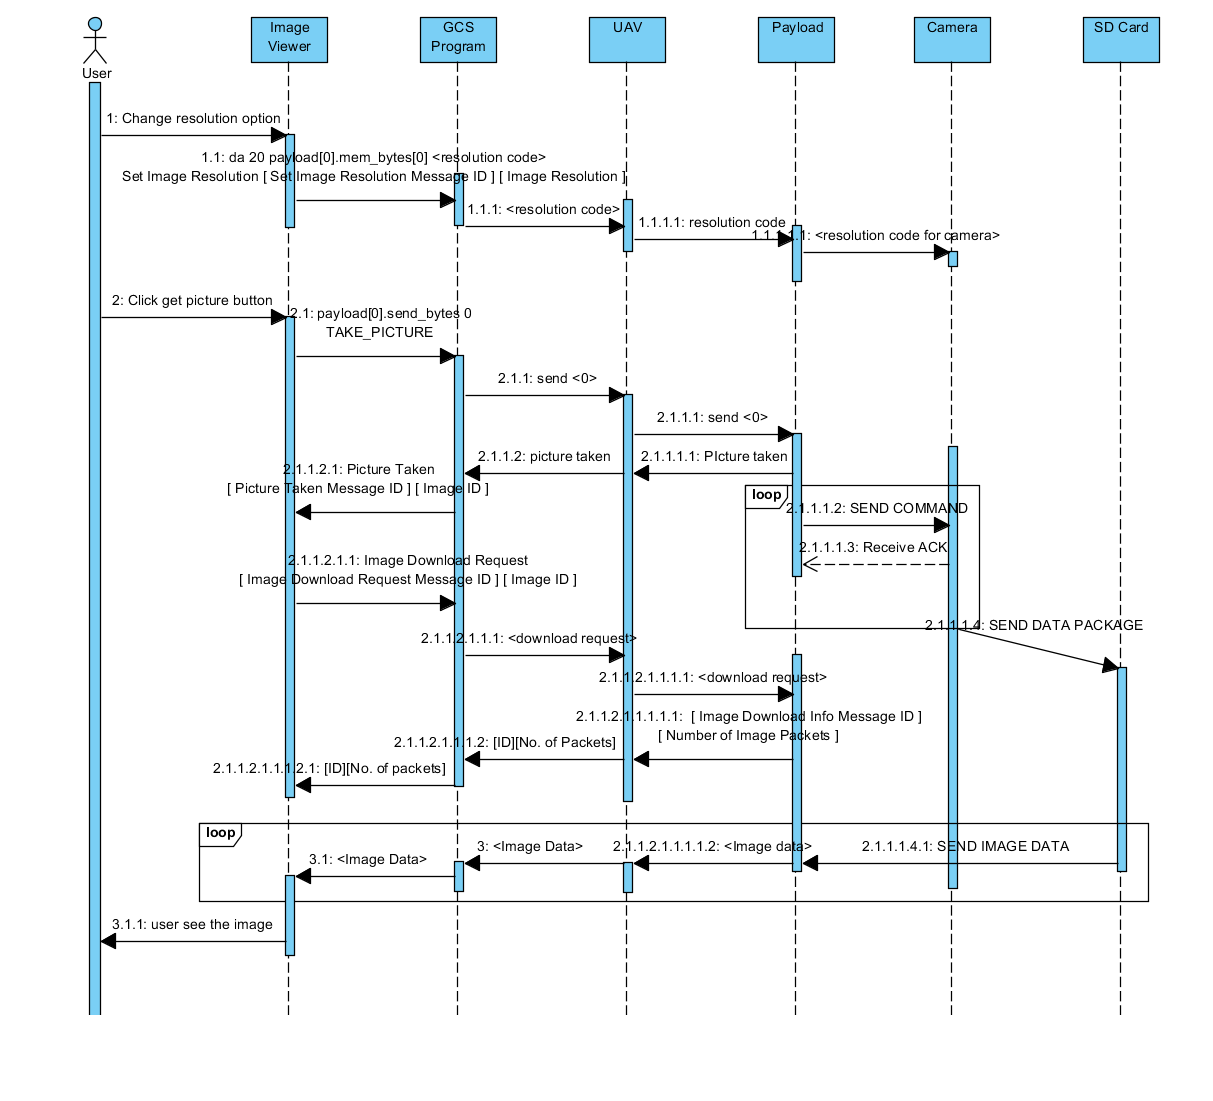
\includegraphics[width=1.00\textwidth]{figures/sequence_diagram.png} 
\end{center}
\caption{Sequence Diagram of the Data flow\label{sequence diagram}}
\end{figure}

Image data is also sent in the same basic manner, however the image is broken up into `packets' of data
which can be placed into the shared memory of the autopilot one at a time, as described by the \emph{Image Data}
message described above. One packet is sent for every transmit token sent by the autopilot, ensuring that the
payload module does not saturate the autopilot link with data. While packets are being sent, the main event loop
still checks for messages being sent from the ground station, allowing functionality such as the cancel download message 
to be implemented. In this way the payload module can transmit a whole image over the autopilot connection.

The testing of the image sending system is described in section \ref{sec:test_pl_image_send}, verifying the milestones 
as described.

Verification of milestone \ref{sec:ms_pl_img_gs_cam_res} (changing image resolution) can be seen in test \ref{sec:test_change_resolution}. Unfortunately changing colour type (milestone \ref{sec:ms_pl_img_gs_cam_colour_type})  was not fully implemented due to time constraints.

\subsection{Problems Encountered (mh)}
A number of problems were encountered and overcome during the implementation of the payload-ground station
communication code, a few of the most important are reproduced here.

\subsubsection*{Autopilot Bug (ab)}

The Autopilot sends "Transmit" tokens to the payload module every 20ms, 
to which a payload module sent an "ACK" token, even when it does not 
transmit any data. We encountered a problem whereby if our we tried to 
send any data to the payload during an "ACK", the autopilot would stop 
sending any "Transmit" tokens at all, effectively cutting off all 
communication to the payload module.

\begin{figure}[H]
  \centering
  \begin{tabular}{c c}
  \subfigure{\label{fig:testing_sc2_working1}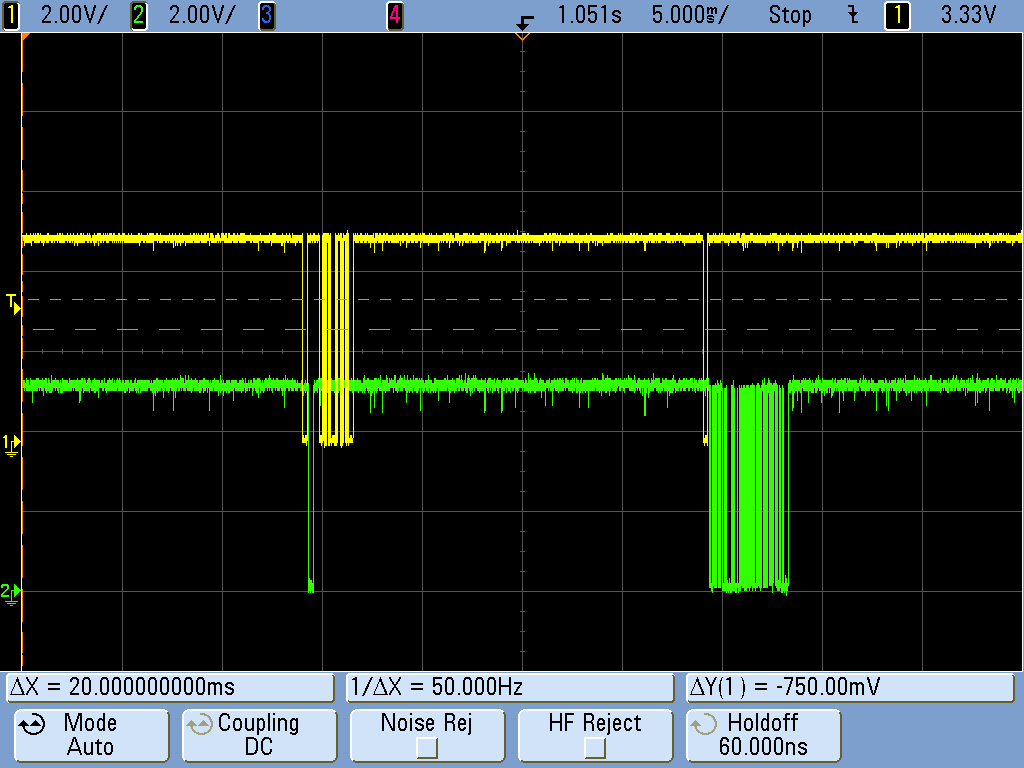
\includegraphics[width=0.5\textwidth]{scope/scope_1.png}}&                
  \subfigure{\label{fig:testing_sc2_working2}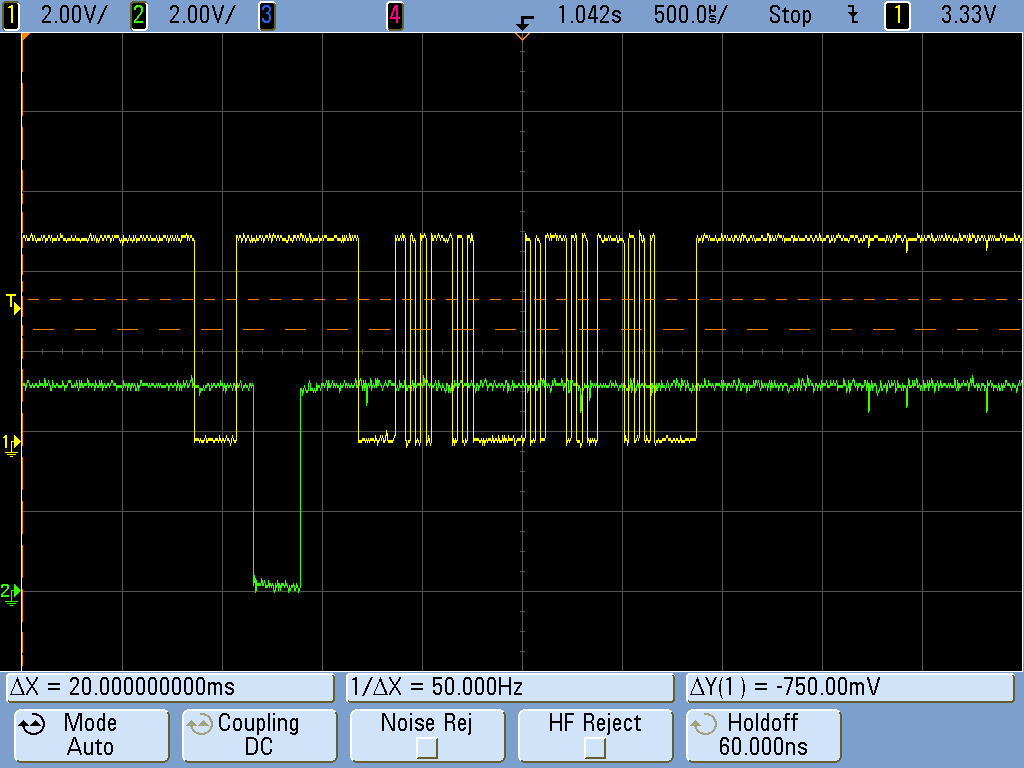
\includegraphics[width=0.5\textwidth]{scope/scope_2.png}} \\
  \subfigure{\label{fig:testing_sc2_working3}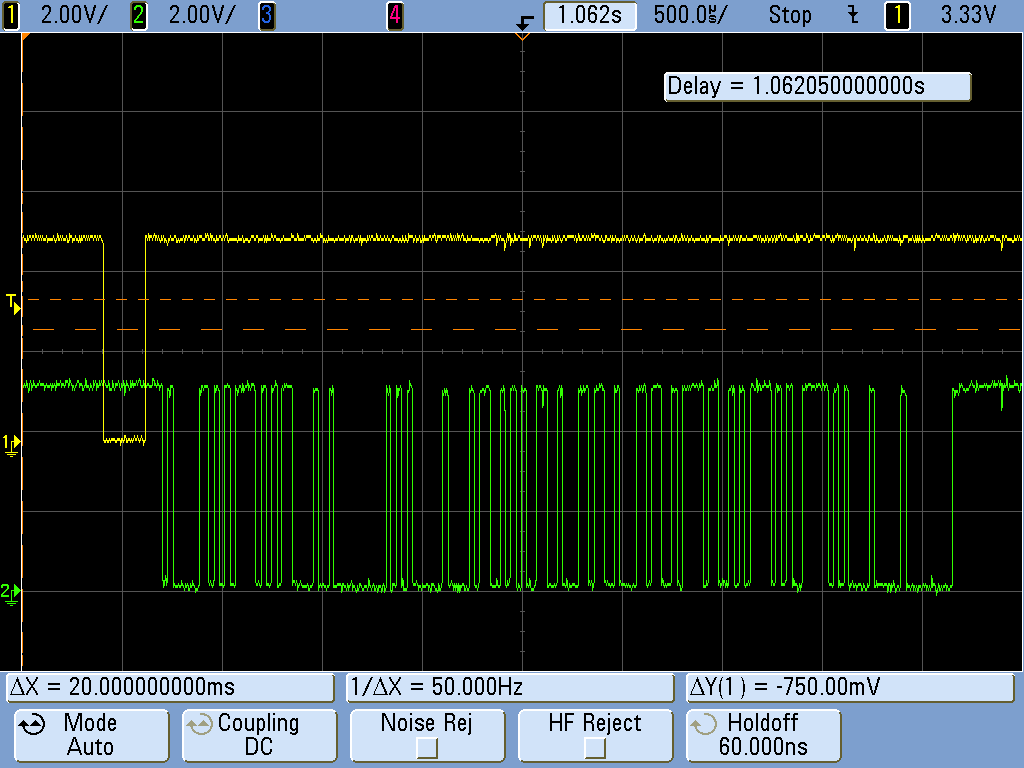
\includegraphics[width=0.5\textwidth]{scope/scope_3.png}}&                
  \subfigure{\label{fig:testing_sc2_working4}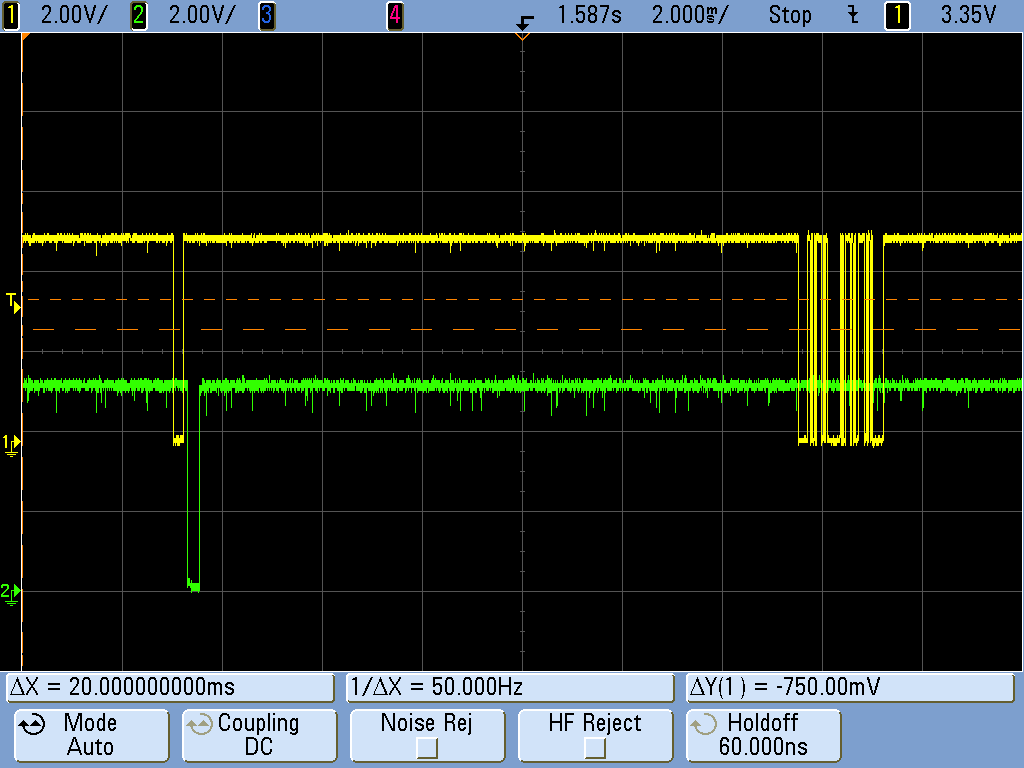
\includegraphics[width=0.5\textwidth]{scope/scope_11.png}}
  \end{tabular}
  \captionof{figure}{Oscilloscope traces for the situation where the autopilot does not break: In yellow is the Autopilot TX, in green the Payload TX. In this situation, after an ACK token is received by the autopilot, a SEND\_BYTES instruction is sent. On the next transmit token, a series of bytes is sent to the autopilot, and the autopilot continues to send Transmit tokens.}
  \label{fig:testing_sc2_working}
\end{figure}

\begin{figure}[H]
  \centering
  \begin{tabular}{c c}
  \subfigure{\label{fig:testing_sc2_broken1}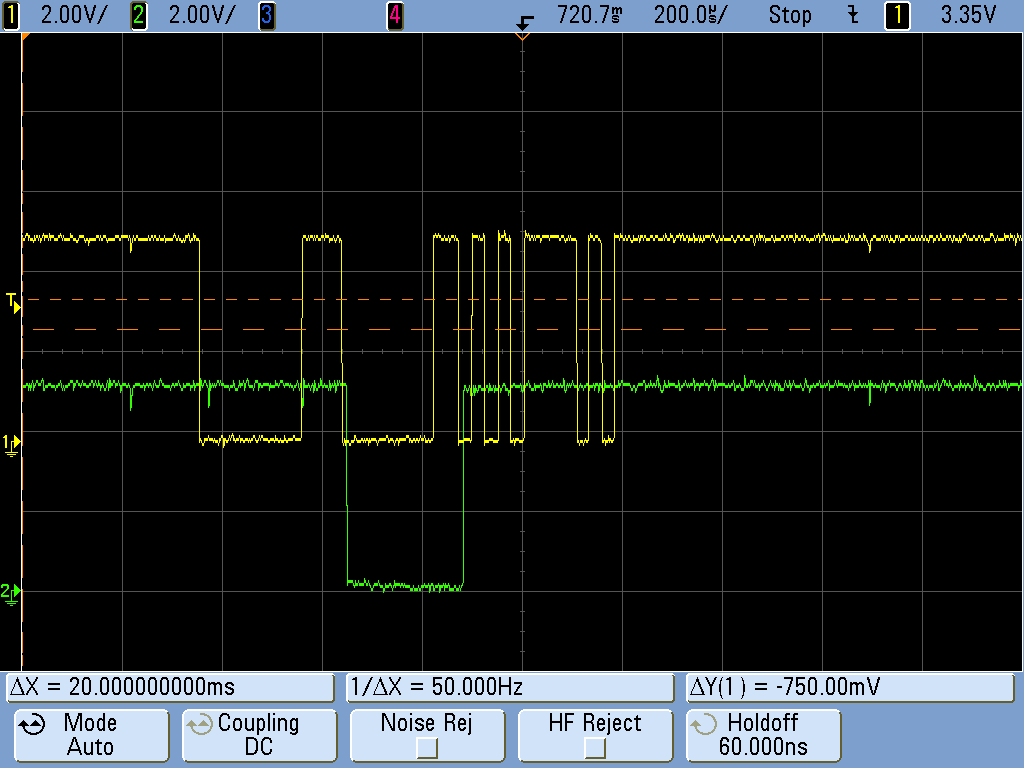
\includegraphics[width=0.5\textwidth]{scope/scope_6.png}}&                
  \subfigure{\label{fig:testing_sc2_broken2}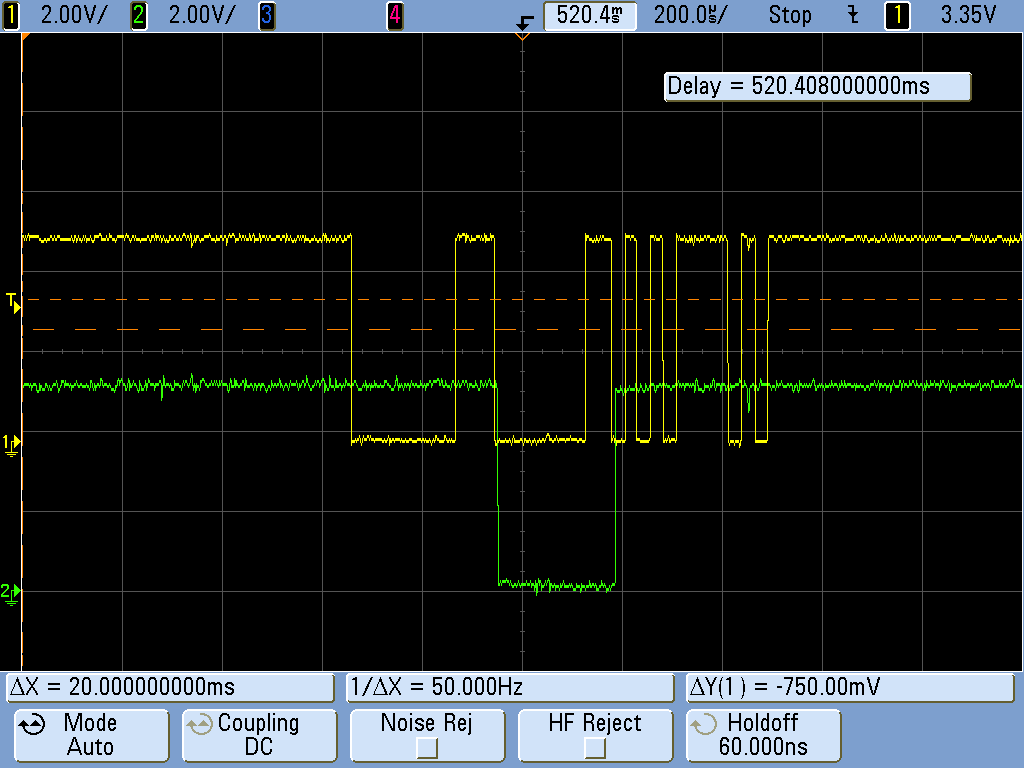
\includegraphics[width=0.5\textwidth]{scope/scope_14.png}} \\
  \subfigure{\label{fig:testing_sc2_broken3}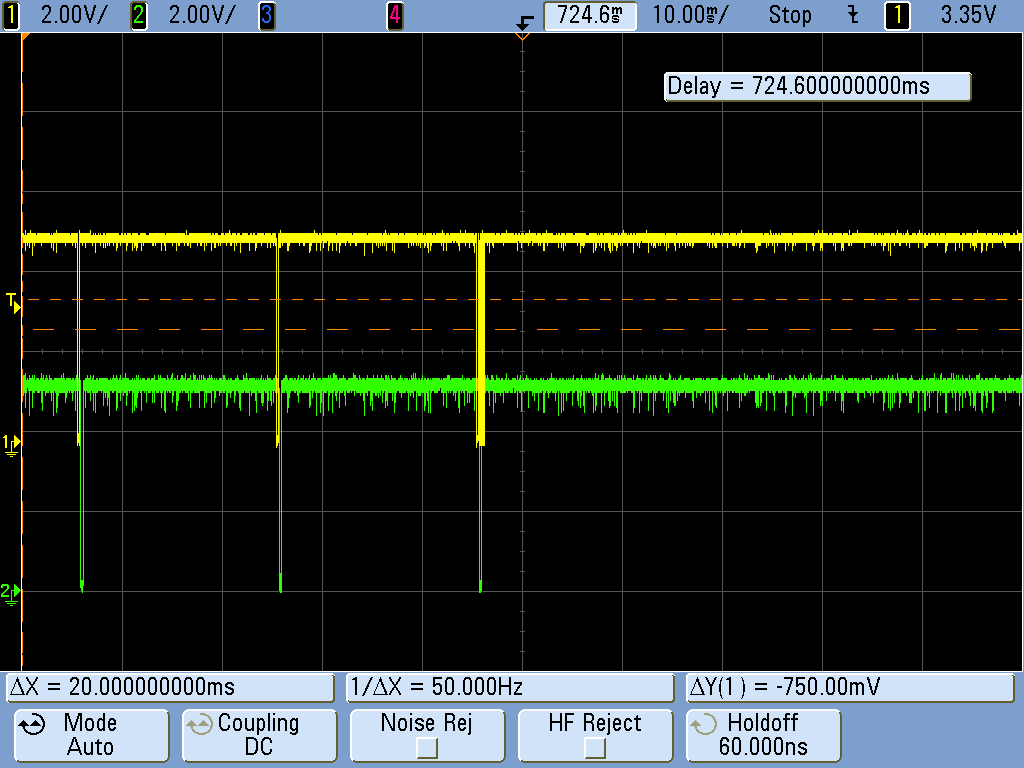
\includegraphics[width=0.5\textwidth]{scope/scope_7.png}}
  \end{tabular}
  \captionof{figure}{Oscilloscope traces for the situation where the autopilot breaks: In yellow is the Autopilot TX, in green the Payload TX. In this situation, whilst an ACK token is received by the autopilot, a SEND\_BYTES instruction is sent. No more transmit tokens are sent, therefore communication with the payload stops.}
  \label{fig:testing_sc2_broken}
\end{figure}

Not sure whether this was a bug with the Autopilot, we got in contact with 
our customer, sending all scope traces to him and a description of how 
to reproduce the error. Not being able to reproduce it with his dummy 
payload (strange, as our dummy payloads only differed in that his used a
surface-mount version of an ATmega168 and a MAX3070 transceiver instead 
of MAX489), he then came to ECS and debugged the Autopilot with us.

After a significant amount of time debugging the Autopilot and our 
payload, it was discovered this was indeed a problem with the Autopilot, 
which our customer was able to fix and subsequently update the firmware 
of our Autopilot.

\subsubsection*{Volatile Variables and ISRs (mh)}

Another problem encountered regarded a flag variable being checked in a function called in the main event loop. The flag
was the continuation condition of a while loop, and although it was being set in another section of code this new set 
value was not being propagated to the while loop code, meaning that the while loop would continue forever. This problem
was discovered (helped greatly by the debug interface described in section \ref{sec:payload_debug_interface}) . After some
consideration, research and experimentation it was discovered that the problem lay with the C compilers optimization. The 
flag was being set in a interrupt service routine (ISR), which the compiler assumed could not be called during the while loop
call, therefore it was optimized out, causing the loop to continue forever. The solution to this was to set this flag variable 
as \emph{volatile}, preventing it from being optimized out in this manner. The same was applied to all global variables modified in ISRs.


%|||||||| REMINDER: PROBLEMS CHALLENGES
%|||||||| REMINDER: HOW DID WE SOLVE PROBLEMS, DEBUGGING, TESTING, ETC
%|||||||| REMINDER: JOHN COULD TALK ABOUT HOW BROKEN CAMERAS SLOWED DOWN DEVELOPMENT BUT GOOD PLANNING AND CONTINGENCY MINIMISED RISK OR IN MANAGEMENT SECTION
%|||||||| REMINDER: FUTURE WORK
%|||||||| REMINDER: ADD NEWPAGES BETWEEN SECTIONS




\section{Progressive JPEG Manipulation}
\label{sec:implementation_progressive_jpeg}
The project planned to incorporate a custom JPEG manipulator which would
take a JPEG image received from the camera and progressively
send the image data to the ground station. 
The planned software would consist of two parts.

The first part of the software would obtain all the information
needed for reconstructing the JPEG image on the ground station.
This would be done using a JPEG image data extractor, and would 
also act to optimize the amount of information sent to the ground station.

The second part of the custom JPEG manipulation
would display the image progessively. 
This would receive the Huffman table information obtained 
from the extractor and use it to reconstruct the image progressively. 
It would then allow the user
at the ground station to evaluate the image as soon as possible,
i.e. before all the image data has been sent. This would also 
save time when combined with the ability to interrupt the 
downloading process of an image from the UAV to the
ground station in case the image appears to be unwanted. 

For information on the reasoning behind implementing 
custom JPEG manipulation, please see 
the JPEG manipulation section in the 
Approaches considered section. \ref{sec:jpegmanipulation}

During the course of the project, only the first part
of the progressive JPEG manipulation algorithm was 
successfully implemented. A form of image displaying 
software has also been constructed which uses the 
Huffman table information obtained from the extractor, 
but a progressively higher resolution display of 
the image was not able to be fully implemented.

\subsection{Progressive Scan of JPEG (commandCheck)}

After receiving the size of the JPEG file (in bytes), 
the JPEG Information Extractor starts reading the bytes of the JPEG stored in the SD card. 
Because the information will not all be available instantly, 
the extractor uses a class to read the next byte in the input stream, one at a time. This class \textbf{read\_byte()} is 
how the JPEG extractor gains access to the JPEG input stream. 

As the extractor reads in the bytes from the input stream, it checks to see if the byte indicates the start of a header (0xff). 
If this is the case, the next byte identifying the header is read and the \textbf{JPEGMethod} class is 
called which uses a switch command to determine the actions to take. 
If not, the data is discarded and the extractor continues to read the next byte is read from the input stream. 

\subsection{Image Data Extraction (JPEGMethod)}

The JPEG Information Extraction class does not need all the possible information that can be extracted from a JPEG image. 
The few image headers containing important information store the important information from the input stream into 
variables which will be sent to the custom encoding algorithm. 

If the header is not recognized by this class, 
it is assumed to not have any important information and is ignored; 
the code continues to scan through the input stream for the next header byte. 
The following headers have  information to be stored (all information is considered to be stored in one byte unless stated otherwise):

\paragraph*{SOF0: Start Of Frame (0xc0)}
\begin{description}
	\item[Data precision] indicates how many bits compose one sample (generally 8 to indicate a byte).
	\item[Image height] indicates the height of the image in pixels (2 bytes long).
	\item[Image width] indicates the width of the image in pixels (2 bytes long).
	\item[Number of components] indicates how many components define one pixel. 
		This will always be three for our cases to indicate the use of the YCbCr colour model. 
		The component information is read in in the order Y, Cb, Cr.
	\item[Component ID] indicates the ID number used by the JPEG file for this component.\footnote{One for each component}
	\item[Sampling factor] both horizontal and vertical are stored within a single byte. 
		The least significant 4 bits indicate teh vertical sampling factor, 
		while the most significant 4 bits indicate the horizontal sampling factor.\footnotemark[1] 
	\item[Quantization Table Number] associates the component to a quantization table.\footnotemark[1] 
\end{description}

\paragraph*{APP0: JFIF application segment (0xe0)}
\begin{description}
	\item[File Identifier Mark] indicates that this is a JFIF standard image.
	\item[Major Revision Number] must be checked to be 1.
	\item[Minor Revision Number] 
	\item[Units for x/y Density] 
	\item[X Density]2 bytes
	\item[Y Density]2 bytes
	\item[Thumbnail Width] Not used.
	\item[Thumbnail Height] Not used.
	\item[Remaining bytes] contains information regarding the image's thumbnail. This is not used in our extractor.
\end{description}

\paragraph*{DHT: Define Huffman Table(s) (0xc4)}
\begin{description}
	\item[HT Information] contains the following information concerning the indicated Huffman Table in one byte:
		\begin{description}
			\item[Bits 0\ldots3] ID number of the HT (cannot exceed 3)
			\item[Bit 4] Indicates whether the HT is DC (0) or AC (1)
			\item[Bits 5\ldots7] Unused.
		\end{description}
	\item[Number of Symbols] is a string of 16 bytes, each byte containing the number of symbols with 
		codes of length 1\ldots16. For example, if the third byte of the string is 7, 
		there are 7 signals of code length 3 in this Huffman Table.
	\item[Symbols] is a string of \emph{n} bytes, where \emph{n} is 
		the sum of all the values in the previous 16-byte string. 
		The extractor stores the Huffman tables in a linked list of struct objects representing the Huffman Tables.
\end{description}

\paragraph*{DQT: Define Quantization Table(s) (0xdb)}
\begin{description}
	\item[QT Information] contains the following information concerning the indicated Quantization Table in one byte:
		\begin{itemize}
			\item[Bits 0\ldots3] ID number of the QT (cannot exceed 3).
			\item[Bits 4\ldots7] Precision of the QT. Either 8-bit (0) or 16-bit (all other values).
		\end{itemize}
	\item[QT values] is a string of \emph{n} bytes, where \emph{n} is $64*$precision$+1$.
\end{description}

\paragraph*{SOS: Start Of Scan (0xda)}
\begin{description}
	\item[Number of components in scan] indicates how many components define one pixel in the scan. 
		This is usually identical to  the number of components obtained from the SOF segment.
	\item[Component ID] indicates the ID number used by the JPEG file for this component.\footnotemark[1] 
	\item[Huffman Table Indicator] stores the AC and DC Huffman Table ID number associated with this component in one byte. 
		The AC Table number is stored in bits 0\ldots3. The DC Table number is stored in bits 4\ldots7.\footnotemark[1]
\end{description}

\subsection{Image Data Treatment}

The SOS Header information extraction segment is followed by 
an algorithm which sorts the image data into chrominance pixels before 
sending the chrominance pixel to the custom JPEG encoding class. 
If we consider \emph{n} to be the number of image pixels in a chrominance pixel, then 
we associate the first $n - 2$ bytes with the Y (luma) Huffman tables, the $n - 1$ byte with the Cb Huffman tables, and 
the $n^{th}$ byte with the Cr Huffman Table. 
This continues until the EOI header is found, or until there is no more bytes coming in from the input stream.


\section{Integration of Payload Sub-Modules (mh)}
\label{sec:int_pl}
%|||||||| REMINDER: DISCUSSION OF ARDUINO MULTIPLEXED SERIAL

\subsection{Integration of Camera Module with SD Card}
Both the camera module and SD card module were initially prototyped and 
partially tested separately,
%|||||| REFS ||||||||
but were integrated at
a fairly early stage. This integration was the easiest way of testing the 
camera module, since the images from the camera could be written to the SD
card, allowing for easy inspection.

\subsection{Integration of Camera Module and SD Card with Payload-Ground Station Communication}
Integrating the camera module with the payload to ground station communications
was a major milestone for the project, since completing it would mean we would
have a basic working system. It was also one of the most challenging parts of
the project. This step was performed iteratively over time, with the most basic
features being implemented, integrated and tested before more advanced features
were attempted

Integration of the Payload-Ground Station communications with the Camera module
was completed on the ATMega644P hardware, please see section \ref{sec:atmega644p_impl}
for more info about this aspect and an idea of the challenges and problems
faced.

\subsection{Integration of Progressive JPEG Manipulation}
Unfortunately due to time constraints we were not able to integrate the
progressive JPEG manipulation code into the payload module, please see section \ref{sec:implementation_progressive_jpeg} for more information.

\subsection{Implementation on Arduino}
\label{sec:implementation_arduino}
Initially we planned to implement the system on the Arduino prototyping 
platform with an expansion `shield' board providing any extra hardware needed -
the reasons for this are discussed in section \ref{sec:appr_considered_arduino}.
The camera module connection code had also already been developed and tested on
the Arduino. 

This plan relied on the implementation of a multiplexed serial solution, where
the single serial port of the Arduino would be used to connect to two different
devices (the camera and the autopilot) at different baud rates and message
formats. It was planned that this would be achieved by the use of tristate
buffers to form a bus with the two devices TX and RX lines. The payload software
could then take care of altering the message format and speed when needed.

Unfortunately, due to time constraints alongside setbacks such as those
discussed in sections \ref{sec:probls_pl} and \ref{sec:cam_prob}
 it was decided that implementing the system on the 
Arduino platform may not the best way to proceed. The main reason for this 
decision was the number of unknowns in the planned multiplexed implementation
- since it was not really how the hardware is designed to be used, it was not
certain it would provide satisfactory results in the limited time that we had.

\subsection{Implementation on ATMega644P}
\label{sec:atmega644p_impl}
Several options were considered alongside the multiplexing option discussed above. One alternative workaround discussed was to use a separate AVR as an interface to the autopilot and connect it to the Arduino using bit-banged SPI or the inbuilt two-wire interface (TWI, sometimes known as I2C). This approach was 
attractive as it meant we could use the existing Arduino code for the camera 
and SD card and use the existing ATMega168 code for the autopilot communication.
However, this solution would add another complex component to the system along
with another communications link, increasing complexity significantly.

Another option considered was using an AVR device with multiple UARTs so one 
could be used for the camera and another for the autopilot link. However, 
the code we had written for interacting with the SD card buffer relied upon 
some Arduino specific libraries. Finding new libraries and rewriting this code 
would be time consuming and inefficient, especially since we had already 
invested time in creating a working SD card solution.

Further investigation into the Arduino SD card library code (for more info
regarding the library see reference \cite{arduino_sd_library}) suggested that
it was coded to work with the ATMega644P chip as well as the ATMega168 and
ATMega328P. Both the ATMega168 and ATMega328P feature only one UART, but the 
ATMega644P features two, making it attractive for use in this project (see
\cite{atmega644p} for more info about the ATMega644P).

Since the ATMega644P provides two UARTs and the SD card library we were using
supported this chip it was decided that using the 644P would be a sensible 
way forward. 

It is important to note that frequent progress reviews meant that the problem of how to implement this integration and the need for 2 serial lines was caught early and controlled before it could become more damaging.

As mentioned above in section \ref{sec:payload_existing_code} the code provided
to us for communication with the autopilot was written for an ATMega168 chip. 
Porting this code and the existing Arduino camera code to the 644P was not a 
trivial task, although it was simplified by the use of the Sanguino library -
a port of the Arduino core libraries to the 644P (see \cite{sanguino}). Some 
changes were made the the Sanguino libraries for use in our project, for 
example the Sanguino handling code for one of the UARTs was disabled to allow
it to be configured manually for autopilot communications. Some small pieces
of code that were causing compilation issues were also modified.

\section{Debug Interface (mh)}
\label{sec:payload_debug_interface}
While the payload module was being developed debugging was a major concern. 
Having access to an oscilloscope very useful when debugging some particularly 
difficult problems.
However, while building the payload module it was clear more complex details 
about the internal state of the program as it was running would be useful.

While prototyping the camera module on the Arduino platform this problem was 
solved by using the \emph{SoftwareSerial} library (for information regarding 
the library see \cite{software_serial}) to send textual debug information via
a serial to USB cable to PC. This proved very useful when prototyping camera
communications.

A slightly different approach was taken when using the ATMega644P. Initial 
testing of the software serial library on this platform suggested that it 
would not work without a significant investment in time fixing it. It was
therefore decided that it would be faster to send debug messages over 
`bit-banged' SPI to a spare Arduino board which then forwarded this data to 
the connected PC over serial. Again, having the use of this debug interface 
proved very useful while implementing the system, and was well worth the 
small amount of extra time taken to develop it.

Figure \ref{fig:debud_conn} shows an example of this debug interface seen on
a serial terminal on a PC.

\begin{figure}[H]
        \centering
        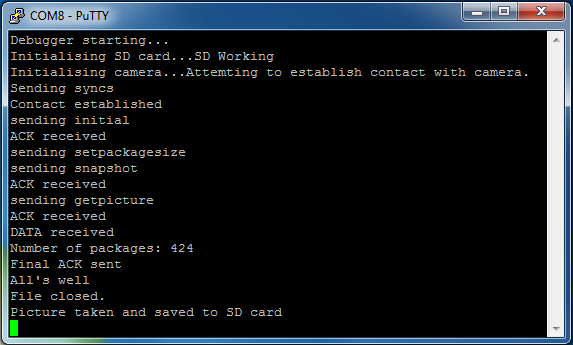
\includegraphics[width=1.0\textwidth]{testing_screenshots/camera_image_saving_sd_card_test.png}
        \captionof{figure}{Debug text sent from the payload over the debug interface.}
        \label{fig:debud_conn}
\end{figure}


%\section{Development Testing and Debugging (mh)}
%The payload module and submodules were tested throughout development in order 
%to ensure the latest changes and features added were working as expected. 
%This allowed bugs to be caught and fixed as quickly as possible, as well as
%increasing our knowledge of the current state and progress of the system and
%project as a whole.

\section{Physical Implementation (ab)}
\label{sec:PCB-implementation}

The final, delivered module is a $88mm\times62mm$ PCB. The PCB manufactured 
for the project was done so for free, using Spirit Circuits' "Go Naked"
service \cite{go-naked}. The PCB itself is a "tracks and holes" only service 
- no soldermask or silkscreen is applied. The schematic of the circuit 
delivered is available in Appendix \ref{Payload_Schematic}, and of the PCB layout in Appendix 
\ref{appendix-layout}. A waterproof lacquer will be applied to the PCB to prevent condensation 
from shorting tracks together, and the module itself presented in a 
waterproof container before flight testing.

A quote of \pounds 56.39 has been obtained from PCB Train \footnote{\url{http://www.pcbtrain.co.uk/quote-and-order-pcb/}} 
for a single PCB, with electrical testing, on a 15 day lead time. 
Please note that Spirit Circuits have only manufactured our prototype 
free of charge on a one-off basis. Being impressed with this service, 
we may recommend that clients contact them for a competitive quote.

\begin{figure}[H]
        \centering
        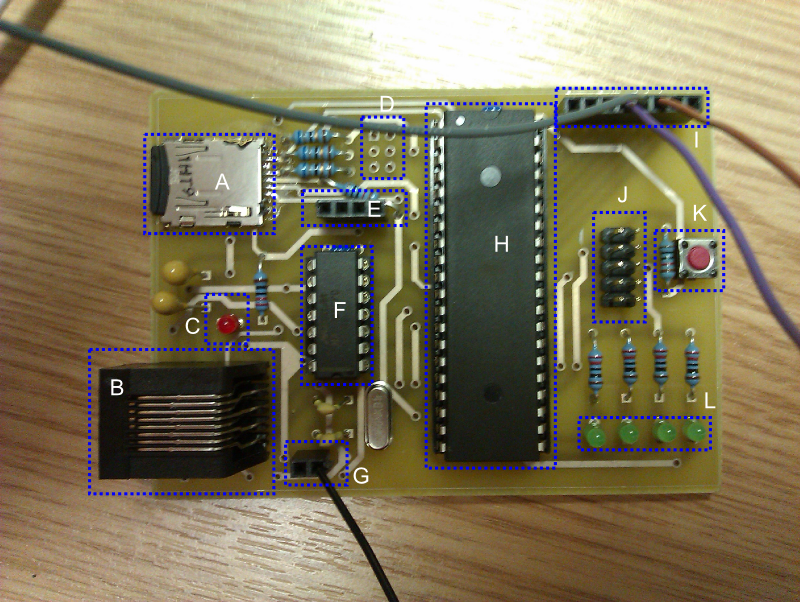
\includegraphics[width=1.00\textwidth]{figures/PayloadImplementation.png}
        \captionof{figure}{Image of the final payload, under test, before lacquer is applied. R11 can be seen between the Camera header and a via near the SD card Vcc.}. 
        \label{fig:PayloadImplementation}
\end{figure}

In figure \ref{fig:PayloadImplementation}, the letters refer to the following 
features of the payload module:

\begin{itemize}
\item \textbf{A:} microSD Card slot
\item \textbf{B:} RJ45 socket, more popularly known as an ethernet socket. 
(Actually implements the RS485 protocol)
\item \textbf{C:} Power LED. Shows whether 3V3 from the ethernet socket is connected.
\item \textbf{D:} ISP programming header socket. As seen, this is not 
soldered on, as we have been using the JTAG header for testing, but will be soldered 
before delivery to the customer.
\item \textbf{E:} Camera header. The camera can be connected to our PCB 
simply by attaching the hook-up wire in the correct order. (L-R: 3V3, GND, 
Camera TX, Camera RX)
\item \textbf{F:} MAX489 (RS485 Transceiver) \footnote{\url{http://uk.farnell.com/9725148}}. 
Cheaper version of the MAX3070 used in the sample peripheral.
\item \textbf{G:} Power header. L: 3V3, R: GND.
\item \textbf{H:} ATmega644P \cite{atmega644p}
\item \textbf{I:} ATmega644P Port A expansion header. (In the image, this is 
being used as a connection to an Arduino Uno so that we may view the debug 
information)
\item \textbf{J:} JTAG programming header
\item \textbf{K:} Reset button
\item \textbf{L:} Debug LEDs
\end{itemize}


%% ----------------------------------------------------------------
\chapter{Implementation - Ground Station (ps)}
%% ----------------------------------------------------------------

\label{chap:implementation_ground_station }

The user can only see the image viewer program.
In order to make the development faster, the console application has been use to test port send/receive information and convert the image data.
The programmer make use of both data stream port and the console port in order to send command and receive JPEG photo from the UAV.

\section{The development process} 
Because GUI include many functions on the application and also it links to TCP/IP ports, the GUI part consider as a very big program. 
Therefore, in order to complete the GUI step by step, it needs a plan for the development.
The connection to datastream can be done by using a console application describe in section\ref{sec:testing_connection_send_to_stream}.
If the connection is correct the appliction can listen to the data stream port as in section\ref{sec:testing_receive_stream}.
These console application will be combined to a bigger and more complete program in later section.

\flushleft
\begin{enumerate}


\item	The most important process of GUI development is to understand what does the customer wants. 

\item	The hardware and software specification have to be determined.
 
\item	Make a GUI design decision

\item Develop a smaller program in order to make the testing easy and less time consuming. 

\item	Learn the .NET class that can support the connection to TCP/IP, and communication between host and device

\item	Use GUI to link to the customer’s software to access the software

\item	Distribute the GUI
\end{enumerate}

\section{Use Case Diagram}
The use case diagram show what functionality the user can use in the program.
It has to include all the specification that the customer want for a complete system.
Figure~\ref{GUI_useCase} shows a possible user action on the program which the user can save, open and delete any jpeg image from the computer. 
The user has an option to connect to the UAV in case of the UAV is not connected properly.
He can command the image viewer program to send an image to the software, and it will display the image onto the picture box.
\begin{figure}[H]
\begin{center}
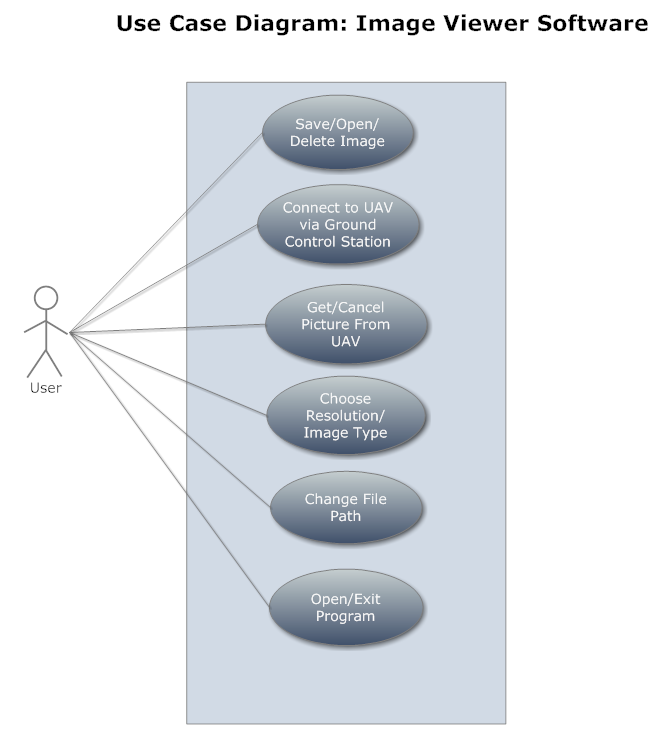
\includegraphics[scale=0.6]{figures/userCase.png} 
\end{center}
\caption{Use case diagram of the GUI\label{GUI_useCase}}
\end{figure}

This initial user diagram has changed because some of the action implement in the background. For example, connect to the UAV function, the user might be confused and click on this button every time the program is open. So the better way to implement this is to make the program connect to the UAV automatically when the program starts running. 
Another changes is the type of image implemented is JPEG only because the raw image will be too big so we decide not to implement it.
Therefore, the Milestone\ref{sec:ms_pl_img_gs_cam_colour_type} will not be implemented.
Figure\ref{GUI_finalUseCase} shows an agreed use case diagram. 

\begin{figure}[!hbtp]
\begin{center}
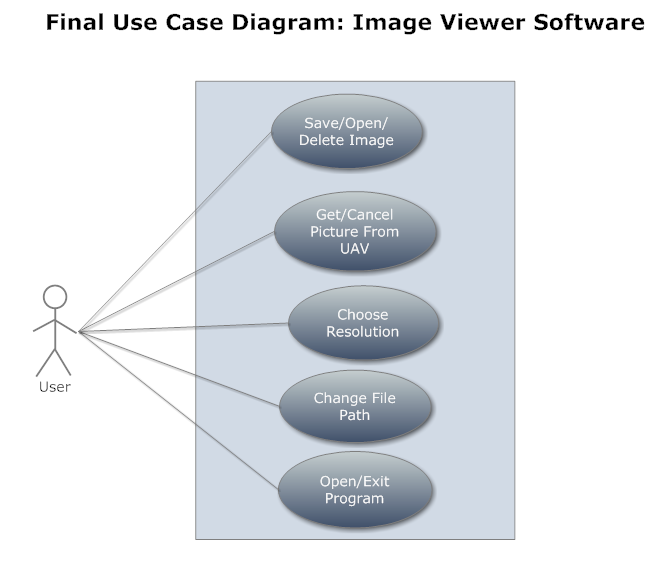
\includegraphics[scale=0.7]{figures/FinaluserCase.png} 
\end{center}
\caption{Final use case diagram of the GUI\label{GUI_finalUseCase}}
\end{figure}



\section{The Design}

The user for our application is assumed to have a limited programming experience, so the program will be implemented so it is simple understand. Figure~\ref{ini_GUI} show the first brainstorm view of the GUI. 
During the downloading process, the application should keep running so the cancel button can be used. 
Gallery button will link to another page which will be the collection of images taken. 
Left and right button can navigate the picture box to view an earlier picture or later picture. 
Cancel button cancel the receiving image, therefore the corrupted picture will not be downloaded. 
The user mode of the application can access only the main feature such as take picture, change directory, and cancel download picture.  
It allows the user to choose the resolution and picture type (RAW or JPEG) to transmitted from the UAV to the ground station. But the user doesn't have access to changing the command, changing the receiving data, and any interaction with the UAV because of safety and avoid of any errors. 
\begin{figure}[H]
\begin{center}
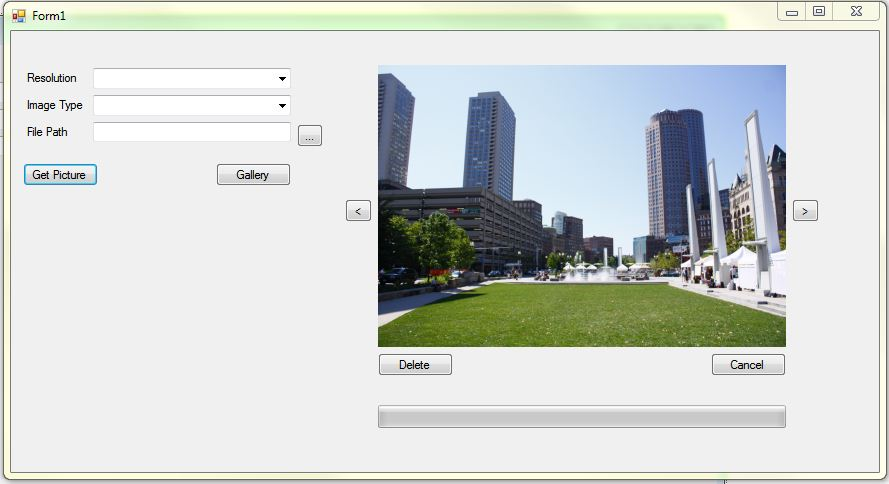
\includegraphics[width=1.0\textwidth]{figures/initialGUI.png} 
\end{center}
\caption{The initial design of GUI\label{ini_GUI}}
\end{figure}
The GUI has been planned to have functions such as auto triggering, image type, resolution type, file path chosen, progress bar, help button, stop and delete. Figure \ref{finalGUI} is the screen shot of the final GUI.

\begin{figure}[H]
\begin{center}
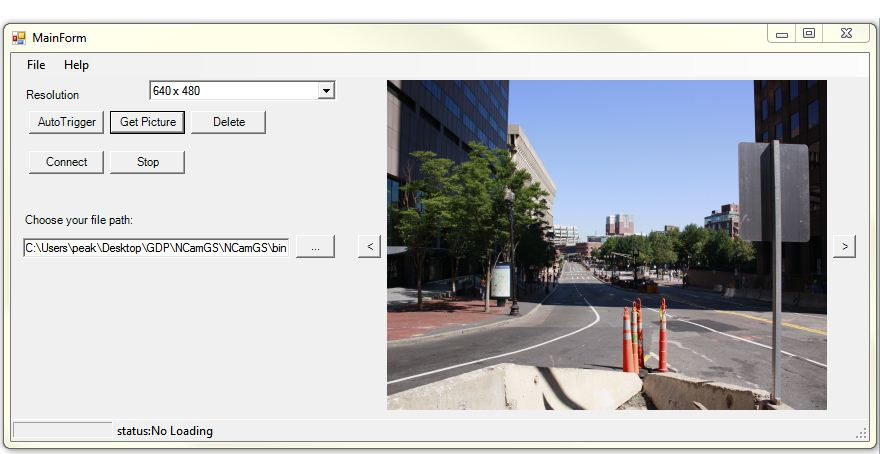
\includegraphics[width=1.0\textwidth]{figures/finalGUI.png} 
\end{center}
\caption{final GUI\label{finalGUI}}
\end{figure}

\section{Class Diagram}
\subsection*{The Initial Class Diagram}
Figure~\ref{ini_Class} shows initial classes and methods of the image viewer program.
The \texttt{JPEGFileReader} Class has functions for decoding/encoding the JPEG file.
There will be decoding/encoding algorithm because the image will take long time to download to the ground station. 
\begin{center}
\begin{figure}[!hbtp]
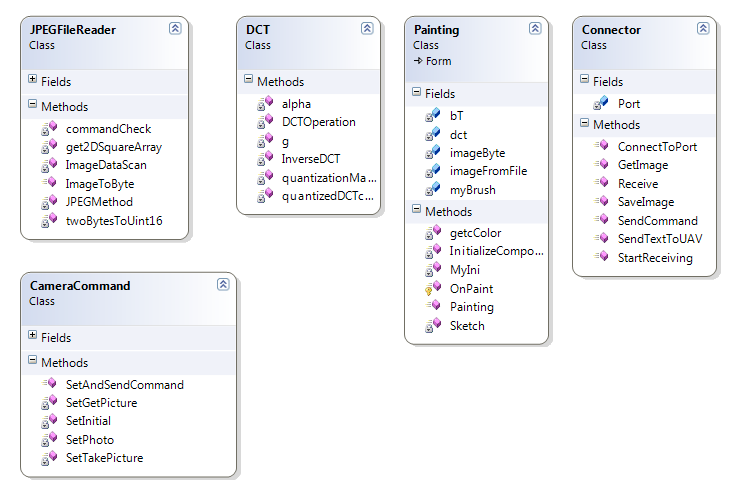
\includegraphics[width=150mm,height=100mm]{figures/initialClassDiagram.png} 
\caption{The initial design of GUI classes\label{ini_Class}}
\end{figure}
\end{center}
\texttt{DCT} class has many math operation and equation which have to be implemented on the image viewer program. 
This complicated function should implement in the ground station because if the picture is encoded in the compressed way, the ground station must be able to extract it. 
In the end, we have to determine whether it is faster to display image normally, or to do encoding/decoding JPEG file. 

The \texttt{Painting} class is supported by the \texttt{DCT} class. The intention of this class is to display an encoded image point by point on the \texttt{pictureBox}.
By this method, the \texttt{pictureBox} can display an image from the first pixel transmitted.

The \texttt{CameraCommand} class design for send the data from the ground station to the camera. The idea is that make the camera sync with the payload by using the ground station command. \texttt{SetAndSendCommand()} use for set the byte command and then send it to the payload via the Console port. \texttt{SetGetPicture(),SetInitial(), SetPhoto(), and SetTakePicture()} methods use for setting the correct byte in order to send the byte by using \texttt{SetAndSendCommand} class.

\subsection*{The Class Diagram}
The class diagram has been implemented very differently from the planned one.
This is because the new plan is to decode the image on board and then transmitted to the ground station in JPEG further compressed file. 
Therefore, the class \texttt{JpegFileReader} has changed to C code and to be implemented on board. 
The \texttt{DCT} class is not needed anymore because all the calculation will be on board. 
The \texttt{CameraCommand} has taken away because the payload will receive an image viewer command to the payload and then the payload will send another different signal to the camera.
Therefore, the command send to the camera from the payload does not have to be the same as the command sent from ground station to the payload. 
The \texttt{Painting} class use to draw each pixel onto the \texttt{pictureBox}, but it has not been implemented in the final program because of the stated reason.
Therefore, the milestone\ref{sec:ms_pl_img_gs_progressive_dl} will not be implemented.
This is also because of the time limitation.
More detail about the progressive image is in the section\ref{sec:implementation_progressive_jpeg}.
 
\begin{figure}[!hbtp]
\begin{center}
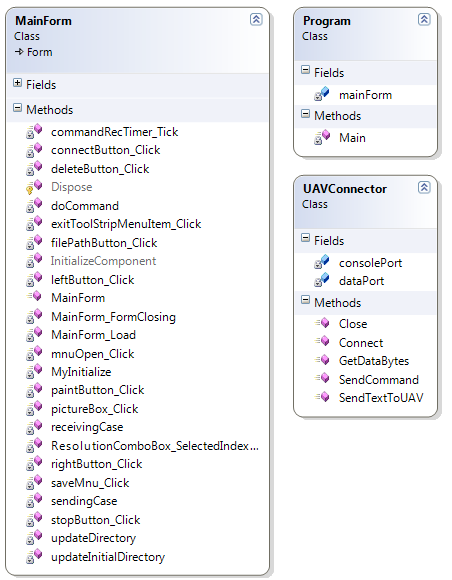
\includegraphics[scale=0.7]{figures/finalClassDiagram.png} 
\end{center}
\caption{Final class diagram of the GUI\label{GUI_finalClassDiagram}}
\end{figure}

\section{Before Connect to the Image Viewer Program}
Figure \ref{schemetic_clipA} shows a diagram of how the connection of the hardware should be. 
The UAV ground receiver is a USB-compatible device which uses Zigbee to communicate. 
USB device driver has been developed by the customer’s so the hardware can be accessed by ground station software, and other applications. 
USB is active when the host ask for a data. 
A host is the computer network which the UAV connect to. 
The data in its queue until the host asks for the data. 
\begin{figure}[!hbtp]
\begin{center}
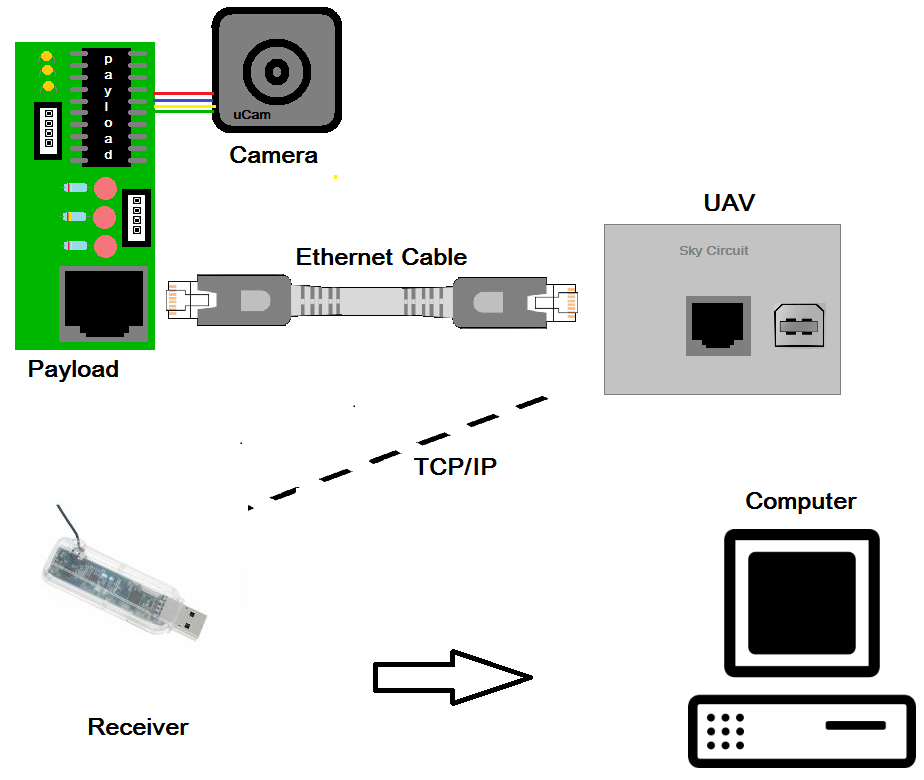
\includegraphics[scale=0.4]{figures/clipArt.png} 
\end{center}
\caption{The connection of the hardware\label{schemetic_clipA}}
\end{figure}


\section{GUI data flow diagram}

Table~\ref{command_table} shows how the command send and receive to/from ground station.  Figure~\ref{GCS_Payload_comm} give a brief detail of how the data communicate between the payload and the image viewer program. 
A more detailed diagram on the data communication is in figure \ref{sequence diagram}.
This has been tested in section\ref{sec:send_console}.

\begin{figure}[H]
\begin{center}
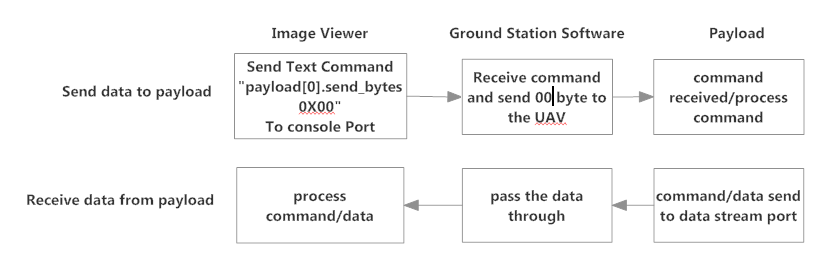
\includegraphics[scale=0.6]{figures/GCS_Payload_communication.png} 
\caption{The connection of data stream port\label{GCS_Payload_comm}}
\end{center}
\end{figure}

\begin{table}[H]

\begin{center}
\begin{tabular}{l l @{.} l}
 Command&
\multicolumn{2}{l}{Address Byte } \\

\hline
\underline{Command from Ground} & \\
SEND\_ZERO\_TOKEN & 0 \\
TAKE\_PICTURE & 0 \\
SEND\_DOWNLOAD\_REQUEST & 2 [MSB] [LSB]  \\
\\
\underline{Command received at Ground}\\
PICTURE\_TAKEN & 1 [MSB] [LSB]\\
DOWNLOAD\_INFO & 3 [MSB] [LSB]\\
IMAGE\_DATA & 4 $\overbrace{ [packet number]}^{2bytes} \overbrace{[image data]}^{data length}$ \\
\end{tabular}
\caption{Command table\label{command_table}}
\end{center}
\end{table}

\section{Get Image Algorithm}
\label{get image algorithm}
In order to take the picture and send it back to the ground station is very important and it has a complex signal algorithm to do.
The plan is when the user click on the Get Picture button, the program sends a \textbf{string command} to the ground station software.
Then the ground station software generates a \textbf{byte command} to transmitted by TCP to the payload. 
Then the payload sends a ''Picture Taken'' command back through the data stream port to the Image Viewer Program. 
Picture taken button has been tested in section\ref{sec:test_get_image_button}
The Image Viewer Program will then automatically send a download request command to the payload. 
The payload will then send image data back to the data stream port. 

When the program start running, the program initialized the port and commands the customer’s application to tell the UAV to stream data to the data stream port. Figure~\ref{GCS_connect_command} shows the connection between the UAV data stream port and the ground station. The UAV has two ports, console port, and data stream port and it can send and receive any length of data. There are some global initializations that the software needs to perform only once when it is loaded for the first time. Note that the console port is manually connected by the ground control station software. The image viewer will give a warning in message box when there is no connection.

\begin{figure}[!hbtp]
\begin{center}
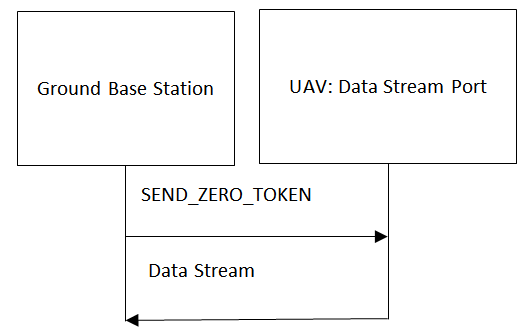
\includegraphics[scale=0.5]{figures/connect_command.png} 
\end{center}
\caption{The connection of data stream port\label{GCS_connect_command}}
\end{figure}


 
\section{Code Highlight}

This section describes the code that is important for the program. The entire code will not be described but it will be in the appendices. It needs a class that can do these to port: connect, receive and send. \texttt{FileStream} class is a class in the .NET C\# which can create a file. \texttt{BinaryWriter} class is use for writing the byte data into a specific file made by the \texttt{FileStream} class. The file directory will introduce a thread. While the open or save a file, the main application must be running, so the application needs to deal with multi threads at the same time. Also when the get picture button got clicked, the main application is frozen because of the thread time organize do one thing at a time. 

\subsubsection*{Connect to UAV:Appendix \ref{appen:UAVConnector} line 18-38.}
The \texttt{Socket} class has functions to send and receive byte and strings data. The handshaking protocol is using \texttt{PortConnect()} method.  
        
The design of the .NET \texttt{Socket} class simply connects to a Port by a single command without any hesitation of changing the baud rate, stop bits, and parity bits. 
This advantage makes the \texttt{Socket} class a more useful class then the \texttt{SerialPort} Class to work with the Port with existing and static set up. 
This class has been tested using a console application before implementing it in a final GUI. 
This will complete milestone\ref{sec:ms_pl_tx_token_resp}.

\subsection{Start of the program: Appendix \ref{appen:main_form} line 78-87}%
In order to make the file name different and meaningful, the name of the picture will be the time and date of the time taken the picture. The code \texttt{DateTime.Now} generate a string of date and time of the current time. This has been done using the date and time class. \texttt{FileStream} was initialize to be in \texttt{FileMode.Create()}, so it can create file. The BinaryWriter write the binary byte into a file in the directory of the fileStream. \texttt{string fileName = string.Format("uavPictureAt{ 0 : yyyy-MM-dd\_ hh-mm-ss-tt}
 .jpg", DateTime.Now);   }  
This code time setting is valid for a file name because it is not using any symbol that will make the program confuse with a code. 
It will display year, month, date, and time in this order. 
The \texttt{BinaryWriter} class can create a binary file using specific data layout for its bytes. 


\subsection{Text Command:Appendix\ref{appen:UAVConnector} line 68-85}
TCP/IP protocols transfer data without modifying them. This allow the application to freely encode the data.\cite{davidB}.The Ground station software allow the program to send a stream of string in bytes and it will read the command bytes and send it to the payload on the UAV. The code has shown the way to implement the string and send a byte array to the payload.

To send text, the string of characters is translated into an array of bytes. American Standard Code for Information Interchange(ASCII) is use for translating English into a binary code. In the \texttt{System.Text} classes provide converting mechanism between each character sets. The \texttt{ASCIIEncoding.GetBytes()} is used for convert character array into a byte array.  
\texttt{The Socket.Send()} method allows the user to send byte stream to the port connected. The customer's program will read from the port and display it onto the command line. The ''@ '' sign indicate that the command correctly sent from the application to the ground station software. The advantage of linking to the ground station software is that our customers can understand what is going on in the console line. For example:uavConn.SendTextToUAV(''da 20 payload[0].mem\_ bytes[0]'');
\ref{sec:ms_pl_shared_mem_set}

The text \texttt{''da 20 payload[0].mem\_ bytes[0]''} will be converted to char array and then to byte array. The byte array will then send the command to the console port to the payload by \texttt{consolePort.Send(toUAVByte, toUAVChar.Length)}. The customer is familiar with the ground station software program, so he can understand the background of the transmission as well. This will complete Milestone\ref{sec:ms_pl_rx_msg_gs}.

In order to test that the payload receives the same data, we use the oscilloscope to see the signal. The byte display on the payload is the same as the byte data send from the ground station. Therefore, the Milesone\ref{sec:ms_pl_img_gs_trigger} is completed. The different resolutions send different byte command to the payload. The byte command changes if the comboBox options change. Therefore, we can say that Milestone\ref{sec:ms_pl_img_gs_cam_res} has completed.


\begin{lstlisting}[caption={writing binary file},label=lst:writingb]          
	for (int i = 3; i < packetSize; i++)
	{
          opFile.Write(packet[i]);
          numBytes++;
    	}
\end{lstlisting}         

At every cycle of the data being received, \texttt{opFile.Write()} method will write the packet data into the file in the directory. After the cycle finished, the file will be saved and the image will be displayed in the picture box. 

\subsection{Get Picture Button}
This get picture button will use both send and receive function of the program. 
The work flow of the get picture signal show in figure \ref{GUI_finalWorkFlow}.
If the sequence of signal send/receive correctly, the photo that receive from the sky will be display on the photo box in the program.
This will complete Milestone\ref{sec:ms_pl_img_sending_gs}.

\begin{figure}[H]
\begin{center}
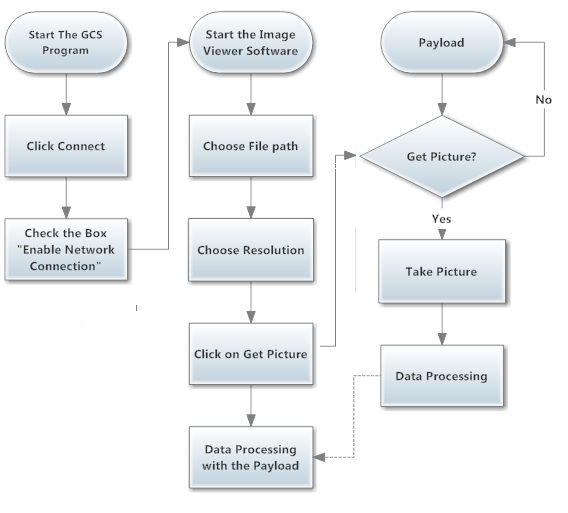
\includegraphics[scale=1]{figures/finalWorkFlow.png} 
\end{center}
\caption{Final work flow diagram of the GUI\label{GUI_finalWorkFlow}}
\end{figure}

\subsection{Implementation - Way-point Triggering (ms)}
\label{sec:waypoint_triggering}

\subsubsection{Description}

The ground station is capable of assigning way-points to
the payload which will allow the camera to take pictures 
at a given location.

This is achieved by sending a simple command script from
the ground station to be uploaded by the payload 
controller. The way-point is designated by the user
through the ground station software. The script 
tells the UAV controller to continuously check the
distance separating itself from the way-point.
When the UAV reaches is within 200 metres of the
way-point, a 0 byte is sent to the camera to prompt
the camera to take a picture.

After taking a picture at the way-point, the camera
is delayed for 10 seconds to avoid taking another picture
at the same way-point. When the 10 second delay is over,
the camera repeats the operation and continuously checks
its distance from the next waypoint.

\subsubsection{Pseudo-code description}

Below is a brief pseudo-code description of the script
sent by the ground station to the payload to take an
image at designated way-points:

\begin{itemize}
	\item while !(UAV distance from next way-point $le$ 200 metres)
		\begin{itemize}
			\item Do nothing.
		\end{itemize}
	\item end while
	\item Prompt camera to take an image.
	\item wait 10 seconds
	\item Re-enter while loop
\end{itemize}

\subsection{Other functions}
The user might want to delete some unwanted photo, so the delete button have been implemented. The delete button work like a normal file deleting button. But it has been complicated because the photo to delete must be the photo on the pictureBox. There is an error because the photo is using by the pictureBox. To fix this problem, the picture have to shifted left or right first and then delete the photo. But where there is only one picture in the file, the program is not allow to delete because even the pictureBox is set to null, its last memory is still point at the deleting file. However, the disadvantage of the delete button is that if the wanted photo got deleted accidentally, it might take a long time to launch the UAV again and take the same photo. The program can also detect the corrupted image and ask the user to delete it.

\begin{figure}[H]
\begin{center}

\includegraphics[scale=0.5]{figures/resolutionOption.png} 
\end{center}
\caption{The resolution in combo box\label{resolutionOption}}
\end{figure}
The camera has options of resolution as shown in Figure\ref{resolutionOption}. This can be useful when the speed is important. The lower the resolution, the faster the data transmitted to the ground. GUI has the combo box for the user to choose any wanted resolution in the options. The resolution allow user to have more accessible to the camera. However, this mean there is more on the programmer side to program the application.


It takes around 8 to 20 seconds to transmit an image of resolution 640x480. This progress bar tells the user how much percentage of data received. The progress bar update at each cycle of the data receives. The status text tells the user what signal have been sent or received. Figure\ref{progressBar} shows the status text ensures that the picture is downloading. However, these have to implement every cycle of the data collection and it might cause the cycle to run slower. The actual loop is much faster than the 38.4kbaud, therefore there is no problem implementing these in.
\begin{figure}[H]
\begin{center}
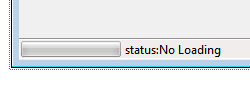
\includegraphics[width=0.3\textwidth]{figures/progressBar.png} 
\end{center}
\caption{The resolution in combo box\label{progressBar}}
\end{figure}

\section{Complete System}
After all the implementation has completed, all the function will be tested together. All the smaller program that we have implemented will be combined at this stage. The send and receiving will use to implement the communication between the payload and the Image Viewer Software. The display of image data will implement as a final display of the image.  Figure \ref{completeSystem} shows a final working GUI of our program. 
\begin{figure}[H]
\begin{center}
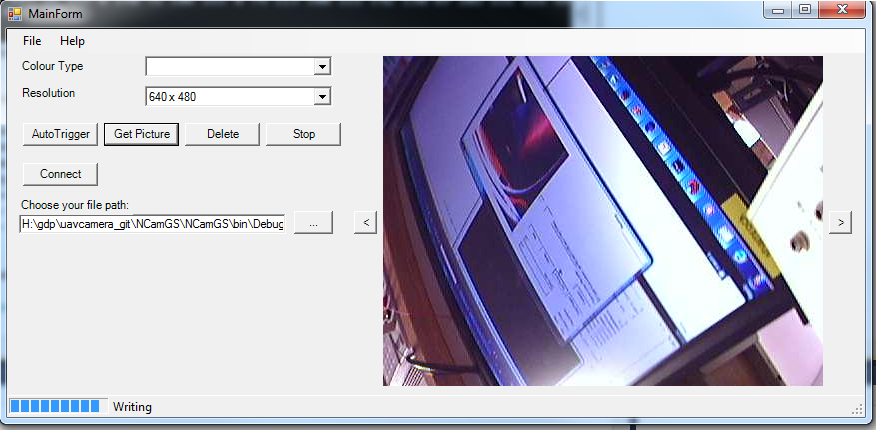
\includegraphics[width=1.0\textwidth]{testing_screenshots/ui.png} 
\end{center}
\caption{The complete system\label{completeSystem}}
\end{figure}




%% ----------------------------------------------------------------
%\chapter{Implementation - Whole System}
%% ----------------------------------------------------------------

%\section{System Integration}


\newpage
% This is part of the FinalReport document.
% Copyright (C) 2011 Piyabhum Sornpaisarn, Andrew Busse, Michael Hodgson, John Charlesworth, Paramithi Svastisinha
% See the file COPYING in FinalReport/ for copying conditions.

%% ----------------------------------------------------------------
\chapter{Overview of Final Progress}
%% ----------------------------------------------------------------

By prioritising and carefully tracking progress throughout the
project a significant number of the goals of the project have been
fulfilled:


\begin{itemize}
	%\item The image should be encoded in such a way that a low quality image will be available quickly, the quality of which would improve as more information is downloaded. [high priority]
	\item Minimise the time needed to download the images from the UAV to the base station. The time from the user’s prompt until the image has been fully downloaded will be measured against the theoretical 3 minutes necessary to transmit a full image without using any compression. The goal will be to obtain a full image in \textbf{less than 3 minutes.} [high priority]
	\item The module weight will be \textbf{less than 250g}. [medium priority]
	\item Image resolution of \textbf{$640\times480$}. [medium priority]
	\item Allow the user to perform the following actions on the UAV’s camera from the base station:
	\begin{itemize}
		\item Prompt the UAV to \textbf{capture and download an image}. [high priority]
%		\item \textbf{Cancel} the downloading of any image while the image is being downloaded. [medium priority]
%		\item \textbf{Resend} an image in case the current preview is corrupted. [low priority]
%		\item \textbf{Interrupt} the download of an incomplete image and allow the user to save the incomplete image. [low priority]
		\item Select the \textbf{resolution settings} of the image. [low priority]
		\item Display a progress indicator which will show the percentage of the image datareceived, as well as a time estimate for the rest of the image to be downloaded. [low priority]
		\item The image capture will be triggered automatically by the UAV using triggers built into the autopilot. [low priority]
%		\item Allow the user to command the image capture to \textbf{trigger periodically} over a \textbf{userspecified time interval} will be added if time permits. [low priority]
	\end{itemize}
	\item Images will be transmitted in \textbf{colour} as opposed to black and white. [low priority]
%	\item The user should be able to select between a colour image and a black and white image. [low priority]
\end{itemize}

We have also produced the requested deliverables:

\begin{itemize}
	\item \underline{Hardware}: Camera module, constructed on PCB (if time permits, otherwise on strip-board),including layout designs.
	\item \underline{Software}: All firmware for the electronic module, and software on the base station for viewing images. The full source code and all executable files will be included.
	\item \underline{Documentation}: Technical and User Documentation. This includes all schematics related to hardware as well as all other documents concerning both the software and hardware delivered.
	\item \underline{Public repository}: The full source code, all schematics, and all documents concerning both the software and hardware will be included on a public repository so that the client may share this information with his clients.
\end{itemize}

However, unfortunately due to time constraints we could not complete
some of our goals:

\begin{itemize}
	\item The image should be encoded in such a way that a low quality image will be available quickly, the quality of which would improve as more information is downloaded. [high priority]
	%\item Minimise the time needed to download the images from the UAV to the base station. The time from the user’s prompt until the image has been fully downloaded will be measured against the theoretical 3 minutes necessary to transmit a full image without using any compression. The goal will be to obtain a full image in \textbf{less than 3 minutes.} [high priority]
	%\item The module weight will be \textbf{less than 250g}. [medium priority]
	%\item Image resolution of \textbf{$640\times480$}. [medium priority]
	\item Allow the user to perform the following actions on the UAV’s camera from the base station:
	\begin{itemize}
	%	\item Prompt the UAV to \textbf{capture and download an image}. [high priority]
		\item \textbf{Cancel} the downloading of any image while the image is being downloaded. [medium priority]
		\item \textbf{Resend} an image in case the current preview is corrupted. [low priority]
		\item \textbf{Interrupt} the download of an incomplete image and allow the user to save the incomplete image. [low priority]
		\item Select the \textbf{resolution settings} of the image. [low priority]
	%	\item Display a progress indicator which will show the percentage of the image datareceived, as well as a time estimate for the rest of the image to be downloaded. [low priority]
	%	\item The image capture will be triggered automatically by the UAV using triggers built into the autopilot. [low priority]
		\item Allow the user to command the image capture to \textbf{trigger periodically} over a \textbf{userspecified time interval} will be added if time permits. [low priority]
	\end{itemize}
	%\item Images will be transmitted in \textbf{colour} as opposed to black and white. [low priority]
	\item The user should be able to select between a colour image and a black and white image. [low priority]
\end{itemize}

\newpage
%% ----------------------------------------------------------------
\chapter{Testing}
%% ----------------------------------------------------------------

\section{Camera Module Testing - (mh)}

The camera module and controller were tested throughout their development and thus problems were quickly discovered and swiftly rectified.

\subsection{Test: uCam Existing Software (jc)}
\label{sec:existing_software_test}

The uCam has a freely downloadable piece of software (downloadable from \cite{ucam_test_software}) that allows you to test the uCam and verify its functions. If you can connect the uCam to a COM port on the computer then you can sync with it and then take and view pictures in the different available formats and resolutions.

This allowed for not just the functionality of the camera to be verified but said functionality was then compared to the specification and it was shown that the uCam should be able to provide what is required from the camera module.

The uCam was connected to a host PC using a USB to Serial cable and tested using the software. The software connected to the camera successfully and downloaded an image as expected.

This task did not verify any milestones, but it did show clearly that the camera was working. In the event of the camera becoming unresponsive, this software helped us diagnose the problem, since if the camera worked with this software it was clearly a problem with our implementation, while if the camera did not work with this software then it would suggest the camera itself was at fault. Before declaring any of the cameras used in the project faulty they were checked using this software.

\subsection{Test: Basic Connection Test on Arduino (mh)}
\label{sec:basic_connection_test}

The first step when communicating with the camera module is to establish a connection to it.  The implementation code follows the procedure shown in figure \ref{fig:syncProto} to connect to the camera, sending SYNC commands until the appropriate response is detected from the camera, indicating a successful connection and so the success of this test.

\begin{figure}[H]
        \centering
        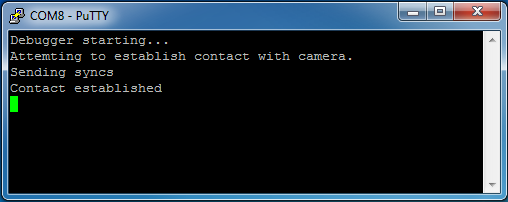
\includegraphics[width=1.0\textwidth]{testing_screenshots/camera_basic_connection_test.png}
        \captionof{figure}{Testing our implementation of the basic connection to the camera module.}
        \label{fig:test_basic_connection}
\end{figure}

Figure \ref{fig:test_basic_connection} shows the result of a test for basic connection to the camera module. In figure \ref{fig:test_basic_connection} the line ``Contact established'' means the Arduino has detected these correct responses. With this successful connection, milestone \ref{sec:ms_basic_cam_comm} is validated, meaning the implementation was free to move on.

\subsection{Test: Image from Camera - (mh)}
\label{sec:image_capture_test}

The first attempt at a simple test for this was to use the debug connection to the Arduino camera controller implementing the camera connection code to relay image data to a PC, unfortunately as described in section \ref{sec:misc_cam_probs} initial implementations of this were not successful, since the debug connection was not completely error free, causing the image to be malformed and unreadable.

However, at this point in the implementation the basic SD card communication had already been implemented and tested as described in section ||||| REF ||||||. Because of this, it was decided  that a much more sensible test would be to write the image data directly to the SD card. The test comprises of running the camera connection code on the microcontroller with the camera and SD card attached. Figure \ref{fig:test_camera_image_saving_sd_card} shows the debug information sent from the controller during this test and \ref{fig:Nyan1} shows the image saved to the SD card. The dedug information suggests that the connection and download of image data was successful and the image on the SD card verifies this.

\begin{figure}[H]
        \centering
        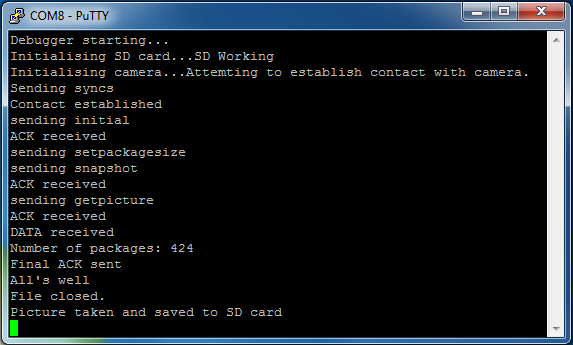
\includegraphics[width=1.00\textwidth]{testing_screenshots/camera_image_saving_sd_card_test.png}
        \captionof{figure}{Debug information sent from camera controller to PC while taking a picture and saving it to an SC card.}
        \label{fig:test_camera_image_saving_sd_card}
\end{figure}

\begin{figure}[H]
        \centering
        \includegraphics[width=1.00\textwidth]{figures/nyanNyan.jpg}
        \captionof{figure}{Test image captured using the Arduino implementation of the camera controller}
        \label{fig:Nyan1}
\end{figure}

The testing during development means that functionality of the controller has been verified already, the test that needs to be performed on this element of the system is to time how long it takes to get an image from the camera and save it to the SD-card and check that this is well within the 3 minutes allowed by the specification. Timing of this process showed that it took around 5 seconds to complete, so well within the 3 minute limit in the specification.

This test verifies milestone \ref{sec:ms_img_from_cam}. The resolution of the image is 640x480.

\subsection{Test: Change Resolution - (mh)}
\label{sec:test_change_resolution}

Since the option to change resolution was a low priority task it was implemented and tested after the basic main system - including image transmission over the autopilot link - was operational.

This test involved sending a Change Camera Resolution command to the payload module over the autopilot link from the ground station, checking the debug line for the correct response and viewing the images downloaded from the camera to verify resolutions.

\begin{figure}[H]
        \centering
        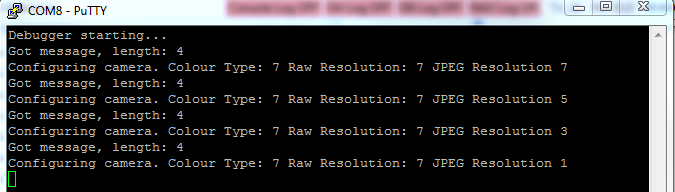
\includegraphics[width=1.00\textwidth]{testing_screenshots/change_res_debug_1.png}
        \captionof{figure}{Test images captured using the integrated implementation of the camera controller}
        \label{fig:test_change_res_debug_1}
\end{figure}

Figure \ref{fig:test_change_res_debug_1} shows the debug information sent from the payload module, the four ``Configuring Camera'' messages in the figure correspond to resolution change messages sent from the ground station. The resolution was changed to the four JPEG resolution values available one after another: 
\begin{itemize}
	\item \textbf{640 x 480}  - Corresponds to ``JPEG Resolution 7''
	\item \textbf{320 x 240} - Corresponds to ``JPEG Resolution 5''
	\item \textbf{160 x 128} - Corresponds to ``JPEG Resolution 3''
	\item \textbf{80 x 64} - Corresponds to ``JPEG Resolution 1''
\end{itemize}

The presence of the debug information recieved from the payload does not validate anything alone, therefore an image was taken at each resolution, shown in figure \ref{fig:change_res_debug}.

This test validates milestones \ref{sec:ms_img_cam_change_res} and \ref{sec:ms_pl_img_gs_cam_res}.

\begin{figure}[H]
  \centering
  \begin{tabular}{c c}
  \subfigure[640 x 480]{\label{fig:whole_fft_lfc}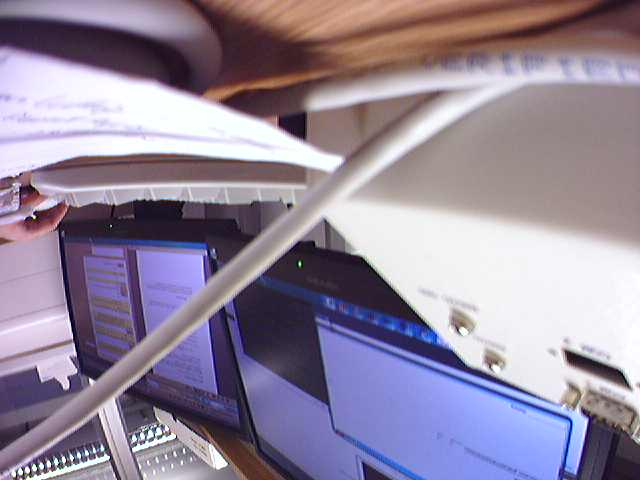
\includegraphics[width=0.5\textwidth]{testing_screenshots/res_pic_640_480.jpg}}&                
  \subfigure[320 x 240]{\label{fig:whole_fft_mfc}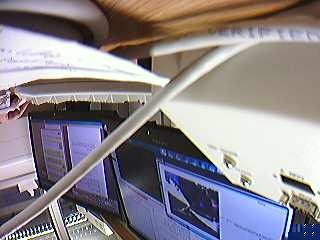
\includegraphics[width=0.25\textwidth]{testing_screenshots/res_pic_320_240.jpg}} \\
  \subfigure[160 x 128]{\label{fig:whole_fft_all}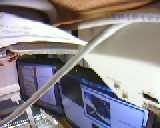
\includegraphics[width=0.125\textwidth]{testing_screenshots/res_pic_160_128.jpg}} &
  \subfigure[80 x 64]{\label{fig:whole_fft_all}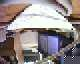
\includegraphics[width=0.0625\textwidth]{testing_screenshots/res_pic_80_64.jpg}}
  \end{tabular}
  \captionof{figure}{Images taken at various resolutions - these were saved by the ground station software after they were downloaded over the autopilot link.}
  \label{fig:change_res_debug}
\end{figure}



%\subsection{Final Camera Testing - (jc)}
%\label{sec:camera_integration_test}

%During the integration process the system was regularly tested for functionality and any errors were fixed as the system was developed. A large number of images were taken during this process and during the implementation of additional features.

%\begin{figure}[H]
    %    \centering
       % 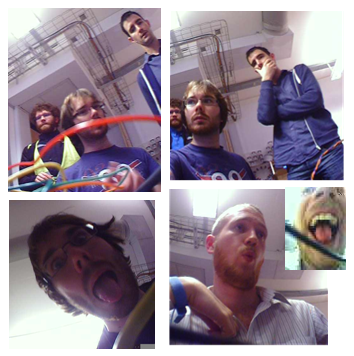
\includegraphics[width=1.00\textwidth]{figures/SampleImages1.png}
       % \captionof{figure}{Test images captured using the integrated implementation of the camera controller}
       % \label{fig:Samples1}
%\end{figure}

%The system can capture images at the 640x480 resolution specified and can also capture images at the other resolutions at which the uCam will take jpeg images. %Currently the option to capture raw images is not implemented.

%The time taken for the system to capture an image at maximum resolution, save it to SD-card and then download and display it on the ground station software was measured at 19.1s |||||||||REF|||||||||. This is still well within the 3 minutes specified and has large amounts of overhead meaning that it should remain well within that limit even if there are+ other payloads implemented on the UAV or if a lot of packets are dropped and have to be resent.



\section{Ground Station Image Viewer(ps26g08)}
\label{sec:ground_station_image_viewer}
The GUI needs a long winded testing. This is because the buttons have to be click and test one by one separately. Because of this, some function of the UAV that does not need a button to test will have its own console application to test it in order to save time. The programmer has to detect most bugs in the real operationThis part is very important because for any program if it caught an error, the program will end unexpectedly.
\subsection{Using Console Application: Testing Connection to UAV, Send Token to Stream Port}
\label{sec:testing_connection_send_to_stream}
The UAV connector use .NET class called System.Net.Sockets. The method that will be using from this class is Sockets.Connect(), Sockets.Send(), Sockets.Receive(). To test the function of this class the programmer develop a separate console application in order to debug only the specific part of the program. Sockets.Connect can be tested by using the Console to display the error code of the running application. The problem could be wrong host name and port number. Therefore, the user are not allowed to change these values. The other problem found in the program is that the programmer forgot to connect the UAV, tell the GCS to enable the enable the network server, and tell the GCS to stream data. Appendix\ref{appen:connectorTest} shows a Connector class that use for testing the Socket connect, read and write method.
Figure \ref{connect to Stream Port} shows a console application testing of the connect function. 
The method is to send a zero token to the data stream and in the GCS program it will display text,\texttt{''\* New datastream client connected from 127.0.0.1:49586''} which it is highlighted in green. 
This text shows that the program works properly and we have accessed to the datastream port of the UAV.
However, the command that send the datastream has not tested in this part. 
This will test the Milestone \ref{sec:ms_basic_dummy_server_comms}.
\begin{figure}[H]
\begin{center}
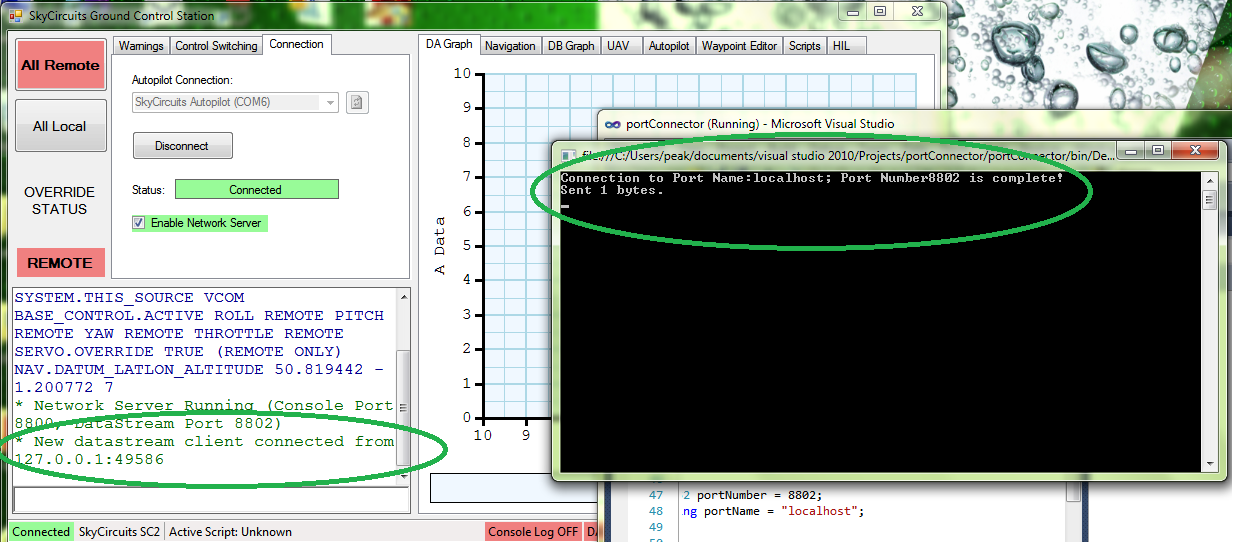
\includegraphics[width=1.00\textwidth]{testing_screenshots/test_sending.png} 
\end{center}
\caption{A screen shot showing the connection with the UAV was successful\label{connect to Stream Port}}
\end{figure}

\subsection{Using Console Application: Testing Connection to UAV, Receive Data from Stream Port}
\label{sec:testing_receive_stream}
Figure\ref{test screenshot} shows a data stream back our testing console application.
Firstly, in the GCS program, we write ''da 30 ht''. 
This code will make the height data stream to the ground station, this data will display on the graph and in the console application, and we can see the number clearly changed when the height has changed.
This is testing that the data stream is working correctly and we have a correct way of getting the data.
Therefore, the Milestone \ref{sec:ms_gs_basestation_comms} is validated.
\begin{figure}[H]
\begin{center}
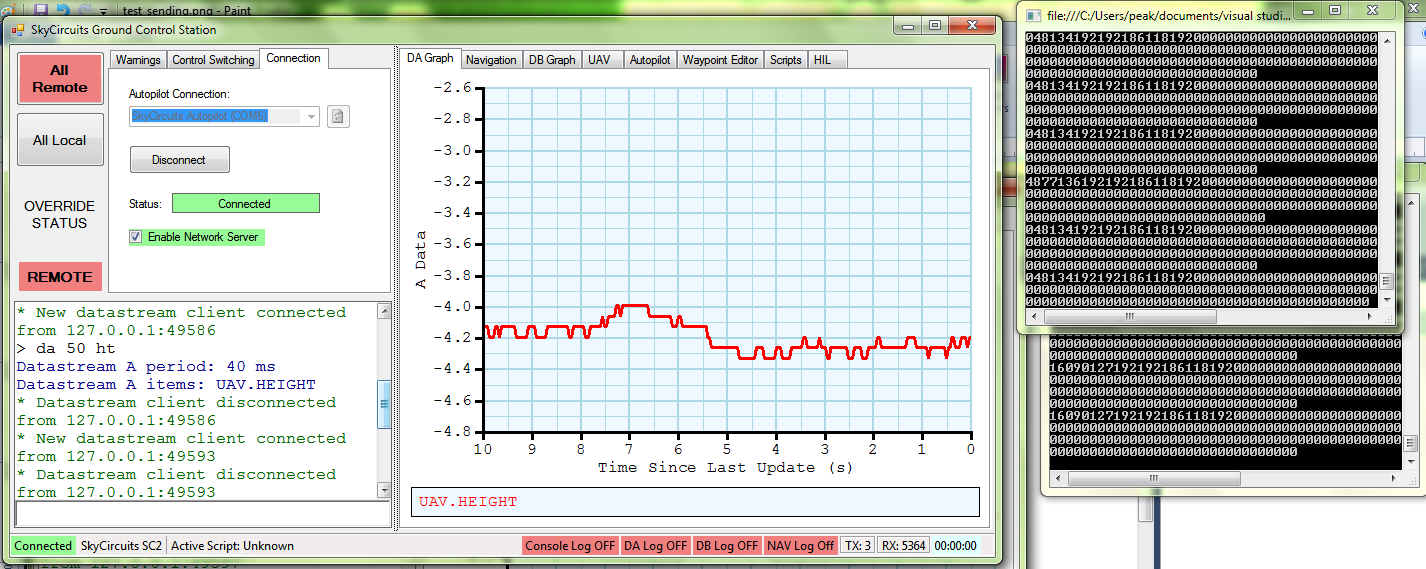
\includegraphics[width=1.00\textwidth]{testing_screenshots/test_data.png} 
\end{center}
\caption{A screen shot shows that the data stream successfully\label{test screenshot}}
\end{figure}

\subsection{Using Console Application: Testing Send Command to Console Port}
\label{sec:send_console}
Figure\ref{test text} show a communication with the console port.
The ground station program allow the programmer to use the console port to send a string command to it. 
This string command can be test that it is correct by the ground station program will produce a line with ''@'' sign on the front of the command sent from the outside of the program.
If the data is correct, the ground station program will detect it and send the data to UAV. 
In the console program, when the user type anything in the console line, it will send byte data to the GCS program.
If the text is a command, the program will process the command and send a byte value as set in the command to the UAV.
The first test is try type 'hi' into the console line.
The GCS will then see the word 'hi' but there is no command available for it.
Therefore, in the GCS console line, it display 'unknown class HELLO'.
Because we send the word via the console line, there is a \@ sign in front of the 'hello' word in GCS program.
The next line we type in is ''da 50 b''.
GCS program know this command therefore it changes the display in the graph to give information about banking of the UAV.
This test validates Milestone\ref{sec:ms_basic_dummy_server_comms}.
\begin{figure}[H]
\begin{center}
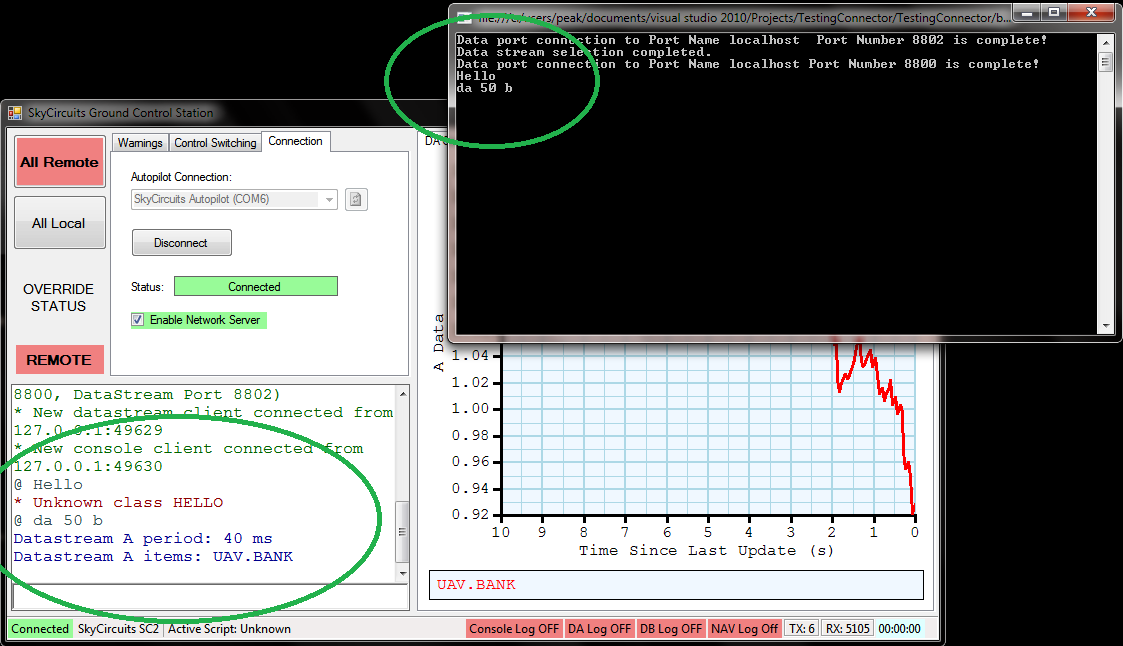
\includegraphics[width=1.00\textwidth]{testing_screenshots/test_sending_test_text_useful.png} 
\end{center}
\caption{A screen shot showing the text sending change the GCS (Ground Control Station) graph value\label{test text}}
\end{figure}

\subsection{Using Window Application: Testing Get Image Button}
\label{sec:test_get_image_button}
The connection between the aircraft and the ground station is using TCP port, it allows the data to send from the aircraft in any form of data. 
In order to test this relationship, a camera will take a picture that the developer know what the picture look like. 
If the picture display an image the same as we expected, the image data is correct.
Figure\ref{camera testing1} shows completed, combined classes together and receive image data.
This testing combined all the existing method together in the Window application.
At this point the connector class will be in the main window application.
When the user click on 'Get Picture' button on the window application, the program will communicate bidirectional, send and receiving which already stated in section\ref{get image algorithm}. 
From the figure, it clearly see that the image is downloading and the image has displayed correctly. This test validates Milestone \ref{sec:ms_gs_recieve_image}. 
\begin{figure}[H]
\begin{center}
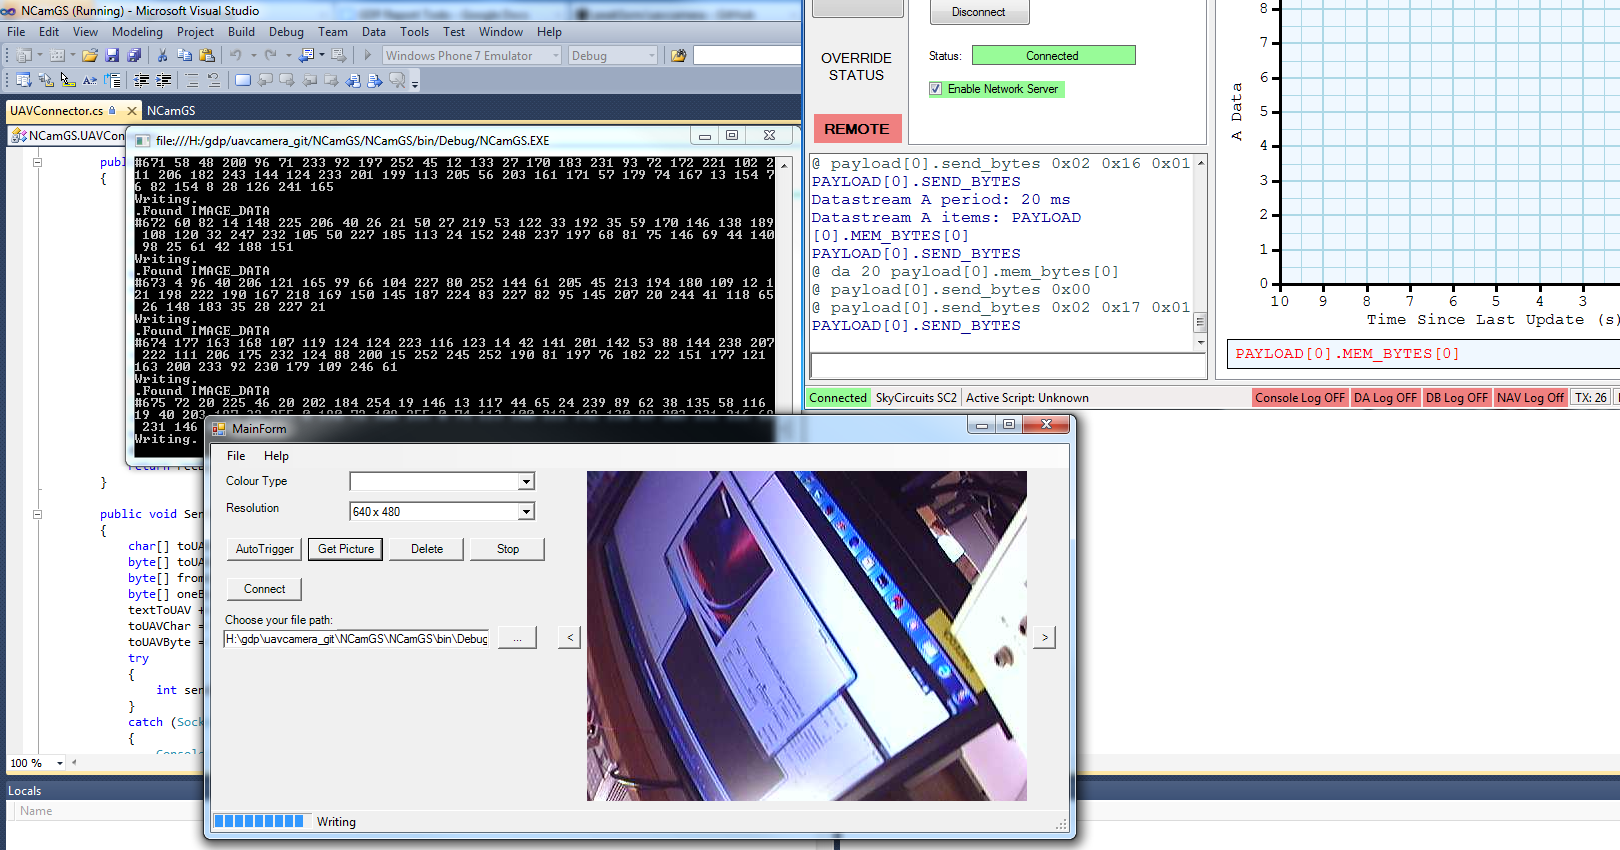
\includegraphics[width=1.00\textwidth]{testing_screenshots/cam_test_11.png} 
\end{center}
\caption{A screen shot showing the picture has been taken correctly\label {camera testing1}}
\end{figure}

\subsection{Using Window Application: Testing Resolution Option}
\label{test_res_op}
When the resolution option changes, the Image viewer program will change the command byte that send to the Console Port of the UAV. 
This can be test by changing the combo box in the image viewer program and click on the Get Picture button.
If it is working correctly, the ground station will see the correct resolution chosen of the picture taken.
Figure \ref{resolution testing} shows a working resolution changing module. 
The putty shows the resolution command that sent back from the payload.
Therefore, it has proved that the resolution option is working.
This test complete the Milestone \ref{sec:ms_pl_img_gs_cam_res}.
\begin{figure}[H]
\begin{center}
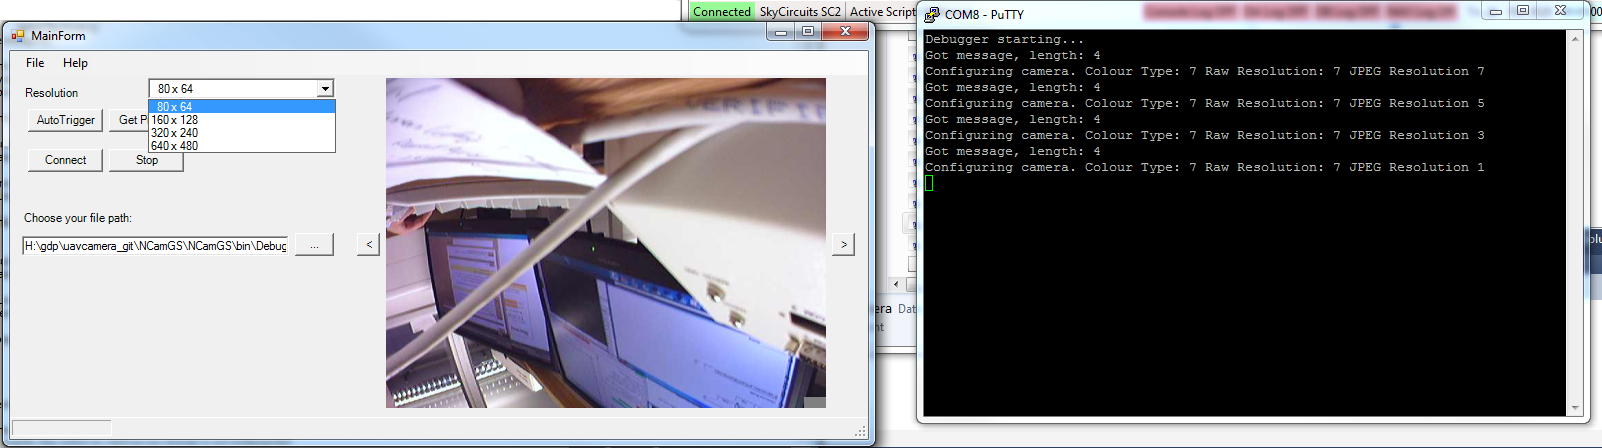
\includegraphics[width=1.00\textwidth]{testing_screenshots/change_res_ncam_1.png} 
\end{center}
\caption{A screen shot showing that the resolution chosen send different signal to the payload\label{resolution testing}}
\end{figure}

\subsection{Functional User Interface}
\label{func_UI}
The tests listed above verifying Milestone \ref{sec:ms_gs_func_interface} is completed. The figure\ref{completeGUI} shows a complete user interface that is functional and ready for the customer to use.
\begin{figure}[H]
\begin{center}
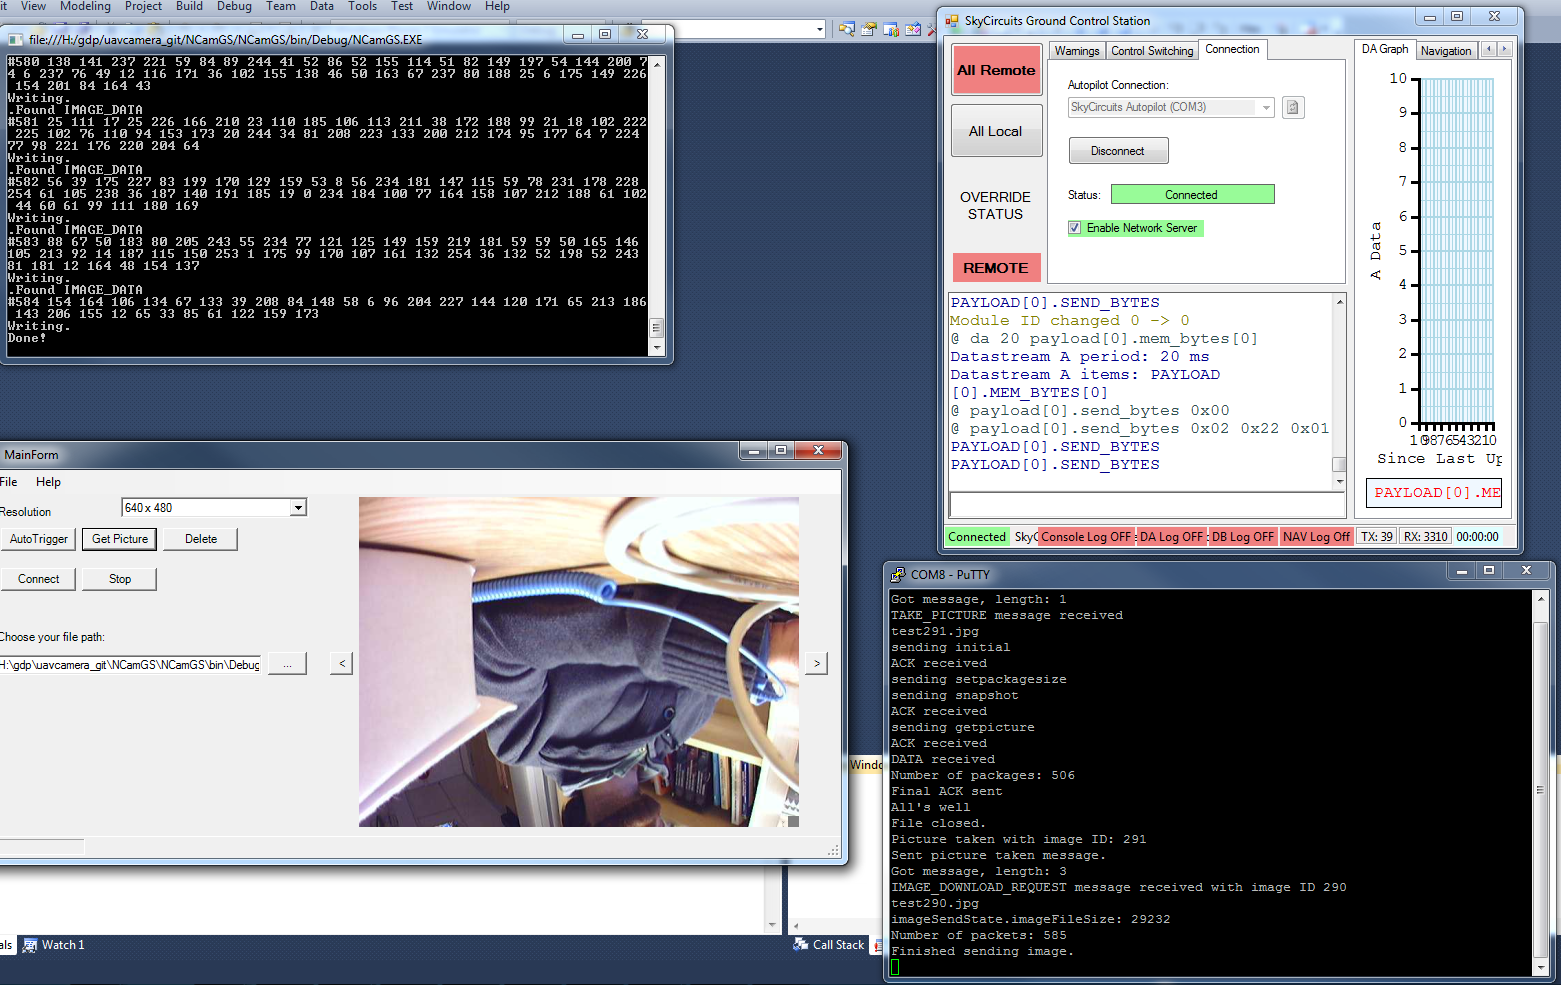
\includegraphics[width=1.00\textwidth]{testing_screenshots/complete_testing_3.png} 
\end{center}
\caption{A screen shot showing a complete UI\label{completeGUI}}
\end{figure}




\newpage
%% ----------------------------------------------------------------
\chapter{Project Management}
%% ----------------------------------------------------------------
Project management goes here...

\section{Gantt Charts}
Michael
Place Gantt charts here.

\section{Risk Management}
Mitch
Place risk management considerations and compare with risks encountered.

\section{Work Allocation}
Peak
Talk about planned work allocation to be compared with actual work allocation. Reflect on efficiency.

\subsection{Planned Work Allocation}
Talk about the tasks planned and the skills audit.

\subsection{Actual Task Allocation}
Talk about who did what in the end and how tasks were passed around. How did people work together?

\section{Team Resources}
John
What we used to get the job done...

\subsection{Budget}
What did we need to buy in the end?

\subsection{Electronic Material}
Did we make use of anything electronic that we had before the project?

\section{Group Communication}
Andy
Talk about how the group contacted each other (email, meetings, mobiles)...



\subsection{Formal Meetings}
Talk about the usefulness and benefit of the formal Tuesday meetings...

For the duration of the project, we held weekly meetings on most Tuesday 
Afternoons from 4pm onwards in the Hartley Library. This allowed us to 
review progress made against progress expected, and to modify our project 
plan and allocation of work for the following week.
\\
Minutes of these meetings are available both in our repository \cite{github} 
(documents/minutes), and as an appendix ?????
\\
The timing of these (the afternoon before our weekly meetings with our 
supervisor) was also quite useful, as it allowed us to present a clear outline 
of new developments and our plans week-by-week.

\subsection{Methods of Communication}
Talk about which methods were used more often, which were useful...

The group has used various methods of communication during the project: 
email, 

\subsection{Source Control}
How we used e-mails, SVN Tortoise, and Github to keep our progress safe...

We decided to use version control software throughout the project, to manage 
everything from minutes to source code and payload schematics. As well as 
being a very useful tool to facilitate group work, it also helps us to meet 
our customer's request to deliver this as an open source project - at the end 
of the project, a repository could easily be gardened and presented, with the 
addition of appropriate open-source licenses at the end of the project.
\\
Initially, we used a central Subversion (SVN) repository hosted on ECS' 
UGForge service. It was decided to use this as most of the group had 
experience using SVN. This worked well for most of the project, but 
unfortunately, something was committed to this repository that could not be 
open sourced (the customer's Ground Control Station software). This presented 
us with a problem, as although it would be trivial to revert this commit with 
the "\$ svn merge" command, this creates a new commit, and the file in 
question would remain in the repository's history and could still be accessed.
\\
In theory, it would be possible to remove this commit from SVN history by 
using the "\$ svnadmin dump" command, filtering the offending commit out of 
the dumpfile, and regenerate the repository with the "\$ svnadmin load" 
command. However, in practice, this was not possible as our repository 
contains binary information above 64kB, therefore the ASCII editor used to 
modify the dumpfile would cut off data in the binary file after the 64kB 
limit, rendering any following data useless.
\\
It would be possible to start a new SVN repository and check in our 
repository up to but not including the offending commit, but we would lose 
all metadata (i.e. committer, commit time, etc.). Therefore, it was decided to 
switch to git, a distributed version control system (which would allow us to 
modify project history). Converting the repository using git-svn was a trivial 
process. Although not all of the group was confident using this tool, git 
lets a committer commit on behalf of another user. Moving to git also 
allowed us to use github, a hosting service, which is free to open-source 
projects (such as ours), which also provides us with some additional 
project statistics. ??? Reference ???? Appendix ???

\newpage
%% ----------------------------------------------------------------
\chapter{Conclusions}
%% ----------------------------------------------------------------

This section will discuss to what extent we have fulfilled the requirements 
of this project, mainly in terms of our initial specification, including a 
justification for why certain aspects were not met, and an analysis of 
whether the project, as it currently stands, could be reasonably presented to our customer as a working solution.

\section{Commented Specification}

The initial specification is available as Appendix \ref{initial_spec}. 

This is then analysed and justified in Section \ref{sec:specification}

\subsection{Fully Completed Parts}

\begin{itemize}
\item \ref{sec:spec_b} : The mean time to download an image, with no packet 
loss, is X seconds ??? reference ???. This figure is obtained from testing 
with the serial link only.
\item \ref{sec:spec_c} : The combined weight of the electronic module and 
board camera is 58g. Combined with the camera enclosure and ethernet cable 
(i.e. the entire additional weight to the UAV to add our module), this is Xg.
?? insert pictures of scales proving this ??
\item \ref{sec:spec_d} : We are able to get an image resolution of up to 
$640\times480$ pixels. Reference the test.
\item \ref{sec:spec_e} : We provide software that prompts the UAV to capture 
an image, download it and then displays it on screen. ?Reference??
\item \ref{sec:spec_f} : Our software is able to cancel the download of an 
image mid-transmission. ?reference test?
\item \ref{sec:spec_i} : Our software allows you to select any resolution that 
is featured on the camera, and download an image at that resolution. ?show test?
\item \ref{sec:spec_m} : We are able to transmit colour images as opposed to 
black and white due to our choice of camera - our camera is only able to 
provide colour images. Therefore it is implemented, but only through our 
choice of camera, not through design.
\end{itemize}

\subsection{Partially Completed Parts}

\begin{itemize}
\item \ref{sec:spec_a} : This task was lowered in priority when we discovered 
that our camera compressed JPEG images a lot more severely than we were 
expecting (image files are approximately 30kB in size, we were expecting 
these files to be 900kB in size). To reflect the time invested in this, we 
have produced some code that partially implements this part of the 
specification, available ???here?
\item \ref{sec:spec_j} : A progress indictor does exist ???ref???, but the 
display only indicates the number of packets received - it does not 
indicate the time remaining to download as this includes the time taken to 
capture an image from the camera and to store it on the SD card.
\end{itemize}

\subsection{Incomplete Parts}

\begin{itemize}
\item \ref{sec:spec_g} : Resending of the same image is not implemented. 
This is, however, a low priority task, which could have been implemented 
if we had more time. In theory, this would be rather trivial to implement.
\item \ref{sec:spec_h} : Interruption of an image mid-transmission and 
saving the incomplete image was again, a low priority task that was not 
implemented due to a lack of time. Again, it should be rather trivial to 
implement.
\item \ref{sec:spec_l} : Automatic image capture at user-specified time 
intervals was another low priority task which we were unable to implement, 
but which should be rather trivial to implement due to the SkyCircuits 
software's scripting interface, but slightly more difficult than the above
two.
\item \ref{sec:spec_n} : Selecting between colour and black-and-white images 
was included in the specification as we considered that this would reduce 
the image transmission time. However, this was not a feature supported 
by our board camera, implementing it on our AVR would be a non-trivial 
process, and the priority to reduce transmission time was reduced as the 
colour image files themselves were much smaller than expected.
\end{itemize}

\section{Deliverables}

This will discuss to what extent we have delivered everything we specified 
in our specification \ref{initial_spec}

\subsection{Hardware}

\ref{sec:deliv_a} : We have delivered a suitable board camera, and an 
electronic module on PCB which interfaces the camera to the autopilot's 
payload port. All schematics, layouts, gerber files etc. are provided in 
our central Github repository \ref{github}, and as Appendices \ref
{Appendix_schematics} and ???

\subsection{Software}

\ref{sec:deliv_b} : The electronic module delivered to the customer is 
presented with firmware loaded on to it, and the user interface software 
presented as an executable file (requiring only that the .NET framework 
is installed on the PC, however this is the same dependancy as for the 
SkyCircuits software). All firmware for the electronic module, as well as 
source code for our executable Ground Station Software, is presented in 

\subsection{Documentation}

\ref{sec:deliv_c} : Documentation for our Ground Station Software is 
delivered with this project ???reference???. It is assumed that our customers' clients are technically competent, therefore documentation on 
how to order a PCB with our gerber files, how to construct the PCB, and how 
to flash an ATmega644P with our source code was deemed unnecessary.

\subsection{Public Repository}

\ref{sec:deliv_d} : All files related to our project are available in our 
central GitHub repository \ref{github}. Most things in there are open-source: source code is licensed under GPLv3 (GNU Public License version 3), 
\ref{gpl}
images (including PCB layouts and schematic designs) are licensed under 
CC BY-SA 2.0 UK (Creative Commons Attribution ShareAlike) \ref{ccbysa}, 
and all documentation under the FDL (Free Documentation License), \ref{fdl}. This is as-requested, and should encourage sharing this information 
amongst our customers' clients.

\section{General Conclusions}

In conclusion, we have presented the customer with exactly what was requested: 
an electronic module that interfaces 

\newpage
%% ----------------------------------------------------------------
\chapter{Evaluation}
%% ----------------------------------------------------------------

\section{Evaluation on Project Management (ps)}

In order to successfully meet the specifications of the project, the task needs to be prioritized so that high priority tasks are implemented before the others.
The tasks with high risk, many dependencies, and requiring the most time to complete were the first set of tasks to be completed.
Because we prioritized the tasks well, we had enough time to implement the high priority objectives of the customer's specification.
Although some low priority tasks were completed some tasks such as the progressive image display have been omitted due to time constraints.

The project management took advantage of group meetings. Each members of the group had to produce a formal documentation in order to keep track of and assign the new tasks.
Some meetings did not have enough progress done beforehand and were not as effective as hoped.
If the group agreed to and managed to implement something on every meeting, it would have made the implementation of the project much faster. 

One thing to be learned from this project is the delivery of components which can be very fast or very slow. 
Therefore, before ordering parts, the group would need to check the delivery time and make sure that the delay had a minimal effect on the progress of work.
The hardware arrived on a slightly delayed and so some members of the team who were assigned tasks related to the hardware were forced to reallocate and perform other tasks while waiting for them to be delivered.
%% ----------------------------------------------------------------
\section{Communication Evaluation (ms)}
\label{evaluation communication}
%% ----------------------------------------------------------------

\subsection{Group Meeting Evaluation}

Having meetings on a weekly basis proved to be very efficient
for the group. Because individual group members met with 
each other on a regular basis throughout the project outside
the weekly meetings, the meetings allowed enough time 
between them to keep them from being redundant.

When certain important deadlines were nearing, the group
would naturally meet up on a more frequent basis and
attempt to tackle important challenges together, even when
no meeting was planned. The meetings allowed the group 
to assess their progress and were vital to avoiding tasks
overrunning.

Minutes of these meetings are available both in our repository \cite{github} 
(documents/minutes), and as an appendix \cite{chap:meeting_minutes}.

\subsection{Minutes Evaluation}

Minutes were taken during each weekly meeting. 
Some minutes were taken during other important meetings 
as well, including meetings with the customer and the 
supervisor. Although, the group member who took 
minutes was not monitored as well as it could have been, 
this did not have any significant effect on the quality 
and/or consistency of the minutes.

The minutes taken were useful for making sure that
all group members were able to check what tasks
they were assigned and catch up on meetings that they
could not assist. The only major setback with the minutes
was the lack of urgency with which they were distributed
to the other group members. Some group members would
update their minutes immediately after the meeting, whereas 
others would not until after the next meeting. Despite
not seriously setting back the project, this undermined the
usefulness of a nonetheless helpful tool.

\subsection{Methods Of Communication Evaluation}

The following methods of communication were used
during the project. One more method of communication
was used in addition to the planned methods.

\subsubsection{E-mail}

For the most part, most of the group members kept track
of their e-mails. On the rare occasion when a group member
became negligent in checking their e-mail, it would either be 
for only a brief period of time, or they would be prompted by
telephone to check their e-mail.

\subsubsection{Telephone}

Telephone was used rarely. Generally, it was used in 
emergencies, for example, 
when a group member was unable to attend a meeting
and could not inform the others by e-mail. It was also
used when members were unexpectedly absent from 
certain important meetings. Overall, e-mail and 
telephone communication complemented each other well.

\subsubsection{Internet Relay Chat}

As the project advanced during the development phase,
more and more tasks required group members working together
in order to be successfully completed. This is due to 
separate modules needing to communicate with each other
and having different people assigned into developing the different modules
in parallel. As this became a more apparent issue, the group adopted
two IRC channels to keep in constant contact with each other.

The first IRC channel was used for development and keeping the 
different module developers in contact with each other as much as possible. 
The second IRC channel was mainly used for the purpose of writing the project
report, due to the large group work involved in creating one cohesive report
from the efforts of different individuals.

Both IRC channels proved invaluable in the later phases of the project, but
due to the individual nature of the early development phases of the project,
were not necessary to be implemented early on. However, it would have been
useful to prepare an IRC at the beginning of the project, if only to have 
another communication tool to help the group members work together.

%% ----------------------------------------------------------------
\section{Encountered Risks (ms)}
\label{encountered risks}
%% ----------------------------------------------------------------

\subsection{Encountered Risk: Faulty Components}
Two major components were found to be faulty very early on. 
The first ordered camera module  
arrived in an unresponsive state. 
Due to the price of the device, 
the group preferred attempting to debug the device before 
ordering a new camera module. 
Eventually however, another device needed to be ordered. 
The second camera module lasted for the majority of 
the development process, but also 
become unresponsive during the final weeks of the project,
after the PCB had been received. 
A third camera was ordered immediately for testing purposes.
Choosing a less fragile camera, or taking special precautions
when dealing with the camera would have mitigated this risk better.

The other faulty component was the autopilot module which 
was given to the group by the customer. 
Due to the nature of the autopilot, being a custom component 
from the customer, it was not possible to simply 
order a new autopilot module. 
The group decided to contact the customer for help, and 
worked with the customer to decode the autopilot software 
as discussed in section \ref{}.

\subsection{Encountered Risk: Team Members Unavailable}
Some members of the team were too occupied to attend 
all the weekly group meetings and 
the weekly meetings with the supervisor. 
However, this was not a severe problem and individual 
members were always willing to allocate 
meeting times when asked directly. 
The group members were willing to warn the others 
when they would be unavailable for a large period of time. 
This issue did not cause large set-backs in the project.

\subsection{Encountered Risk: Difficulties}
Whenever difficulties were faced, the group member 
facing the difficulty would inform the other 
group members about the problem. 
If the difficulty concerns a high priority task, 
the individual group members would reassign 
tasks to make sure that all the high priority 
tasks were completed as soon as possible. 
Thanks to the skills audit (see section \ref{sec:work_plan}), this made sure that 
any difficulties faced in the high priority 
tasks were taken care of. 
\section{Actual Task Allocation(ps26g08)}
In the real work environment, the unexpected situation happens at all time. 
Each members of the group faced different problems.
Some problem was easy to solved but some was very difficult and time consuming. 
The back up plan and unplanned problem solving skills is needed. 
Although many problems happened, but all the team members have been flexible to support each other and most main problems have been solved. Figure\ref{final task allocation} shows an actual work that each member has done in the project

\begin{figure}[H]
        \centering
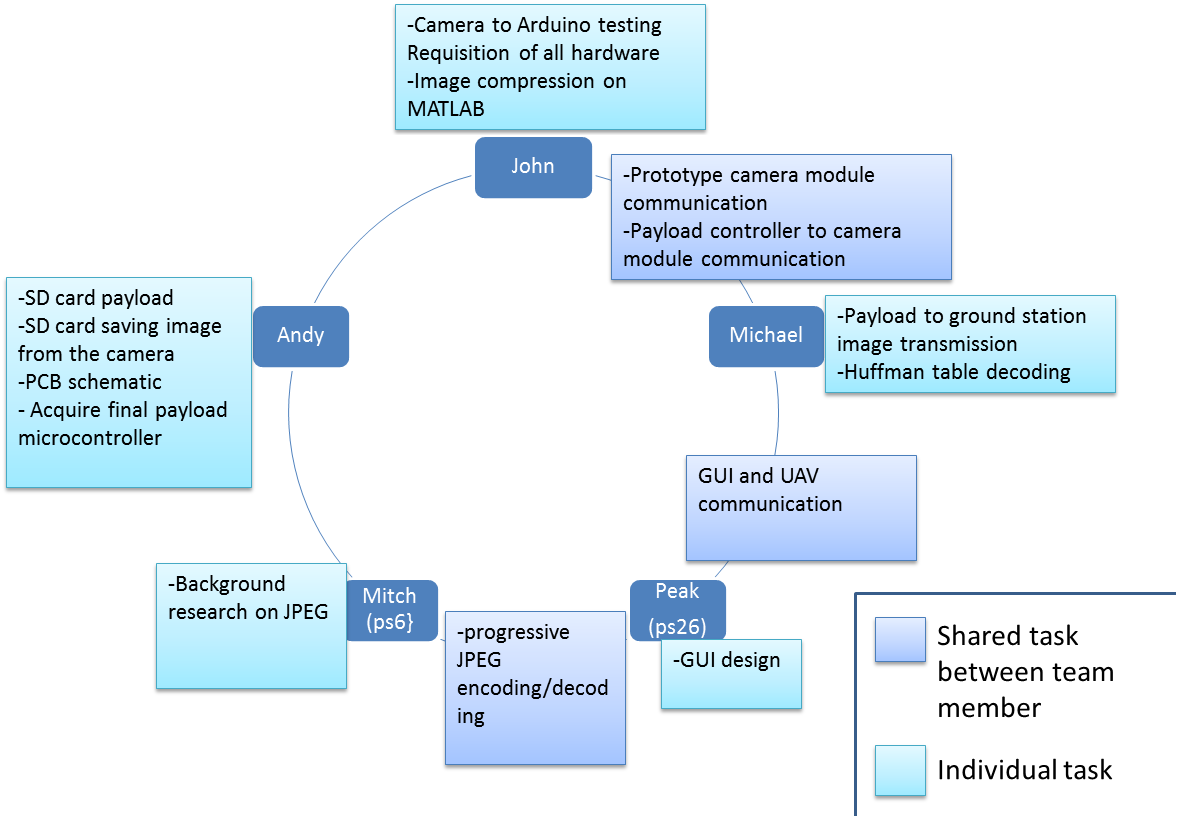
\includegraphics[width=1.0\textwidth]{figures/finalWorkAllocation.png} 
        \captionof{figure}{A diagram show a final work allocation of the team}
        \label{final task allocation}
\end{figure}

Figure\ref{systemBlocD} shows a block diagram of the whole system that the developers has slitted in to blocks of tasks. 

The camera module and other hardware have uncontrollable acquiring time. 
Some of the group members has problem with the delay of the hardware deliveries. Therefore, the time has to extended longer than the gantt chart. 
The solution to this is the software has been developed according to the camera sheet of the hardware. 
And at this stage, the background reading is very necessary so the developers has used this waiting time to plan and develop the software, so when the components arrive, all the task can be implemented.

The task that depend on acquiring the camera are the communication between the payload and the camera,prototype camera module, and image encoding. 
The problem that the developers have is the camera delivered is a faulty.
These tasks has been suspended until the camera have arrived.  
Therefore, the new camera has to be purchased and the allocation of work is necessary. 
There are part that is not depended on the hardware such as encoding/decoding images, and ground station software. 
So the members who were assigning to work on the camera has been allocate to do the software part first.

The payload controller has the problem with the hardware part of the UAV. 
It did not respond to the UAV signal at first. 
Therefore, we assign another group member to support this problems. 
The task leader of this has been assigned to do another software module which have to be implemented. 
This problem also need a support from the customer to update the UAV firmware. 
After problem have been noticed, it has been solved successfully. 

The SD card memory task was considered as a small task in the planned work, but in the real implementation it is very important. 
Therefore, we assign on of the member responsible to this task. 
The SD started to implemented after the camera have been arrive and implemented correctly. 

Because there is only one camera purchased, only one member of the team assign to keep the camera. 
There are problems with the cameras including the delay of deliveries, and camera faulty. 
The task leader of this has been assign to research on the progressive image on MATLAB in order to make a prototype presentation of a compression image taken. 
The task has been delayed from the time set to an individual. 
But after the second working camera arrived, the task has been done beautifully and there is enough time to combine with other tasks.
% This is part of the FinalReport document.
% Copyright (C) 2011 Piyabhum Sornpaisarn, Andrew Busse, Michael Hodgson, John Charlesworth, Paramithi Svastisinha
% See the file COPYING in FinalReport/ for copying conditions.

\section{Evaluation on Project Efficiency (ps)}
The overall design of our project has been done very effectively.
It fully satisfy the high and medium priorities that we has set it.
The project has been done successfully and the outcomes was very pleased by the customer.
However, the project has been changing throughout the time, especially in the hardware part.
The changes on the structure of the payload communication has changed from the planned one.
The SD card has been added to the payload in order to save the picture on board.
It has been described in detail in section \ref{chap:implementation}
The drawback of this is that we have to assign a task leader for this and so the other task might go slower.
In a group, we have already decided that implementing the SD card will be the best use of our time and human resources.
The microprocessor has changed as well as we describe on section\ref{sec:payload controller}.
Therefore, these changes make the whole project much better and more effective.
Every changes in the design means there will be more time spending to recover the task that have been completed. 
Therefore, we could have done the project better if the task was planned at first so there will be no changes in the middle of the project.
Progressive image downloading was the task that was about to implement and we have put many people to look at it. 
It has been proven that it is possible to implement by the MATLAB simulation (section \ref{sec:progressiveimagedisplay}) and also from a lot of research which the team member has been researching(section\ref{jpeg_image_compression}.
Although it seems like a very promising architecture of send the image, the time limitation make this progressive image impossible to implement on the real device.
In the middle of the project, the group meeting has conclude that the progressive image is taking too much of our human resource time and energy.
Therefore, the task has been omitted and there are big reallocation of people to do other tasks.
This might be a big mistake of the group because we have spent a lot of time doing this task.


\section{Project Implementation Evaluation}
\subsection{Image Viewer Software}
%GUI evaluation
In the image viewer implementation, many problems occur and most have been solved.
The program need to wait for many other part to finish before the member can implement the program. 

\newpage
%% ----------------------------------------------------------------
\section{Future work (jc and ab)}
%% ----------------------------------------------------------------

This section of the evaluation looks at potential additions to this project, 
which we would have done if time permitted. This starts with parts of the 
specification that we were not able to implement, and continues with some 
more advanced additions that we have considered.

\subsection{Ground Station Software (ab)}

The Ground Station Software which we have submitted remains rather buggy. 
There is a memory leakage issue which causes both our and SkyCircuits' 
software to crash after viewing a certain number of images, we have not had the time to resolve. This is not altogether critical, as the software 
is functional, and once re-started will re-connect to the autopilot. 
As the autopilot is autonomous, can take control of an aircraft from takeoff 
to landing, and is subservient to a manual controller, this is not a critical 
issue, but one that 

It is also not feature-complete (see \ref{sec:incomplete}), something which 
could be resolved with some fairly trivial modifications to our code.

%% ----------------------------------------------------------------
\section{Progressive Image Manipulation}
%% ----------------------------------------------------------------

The progressive image display was not fully implemented
by the end of the project. Below is a list of possible work
which can be undertaken to complete the progressive
image display system.

\subsection{JPEG Header Extractor}

The information obtained by the JPEG header extractor
has not been completely tested. The DQT information 
has yet to take into account multiple quantization tables
existing within a single DQT segment: only one 
quantization table is read. If a loop and struc similar to 
one implemented for the DHT is replicated for the DQT
segment, the extractor will be able to be tested and
implemented on the AVR.

The AVR implementation will require testing with
the ground station image displayer before it
can make it into a final product.

\subsection{Ground Station Software}

Little work was done for a ground station
progressive image displayer. An application would have
to be coded which will read in the information provided by
the extractor and display the image progressively.
This means that the application would need to reverse the
steps used to compress a raw image into JPEG given the 
coefficients of the Huffman tables and the quantization
tables. 

Attempting to reverse the custom compression of 
raw images MATLAB code using DCT can be a good 
starting point. If successful, reversing the quantization 
and Huffman encoding of the JPEG image would be 
required to obtain the information 
necessary to display the image.

\subsection{Video Streaming (ab)}

A rather interesting advancement of this project would be to try and implement 
real-time video streaming from the UAV. This would almost certainly have to use 
a dedicated wireless link. The 38.4 kBaud available in the autopilot modules 
is too restrictive for this sort of application, but the autopilot would still 
be able to control such an application (i.e. able to start/stop transmission, 
toggle power to the module, minimising delay between video capture and video 
display, 

\subsection{Using Multiple Cameras (ab)}

Another interesting application would be to mount multiple cameras (of the same 
model purchased for this project) on the UAV, and either take pictures from all 
the cameras at the same time, from some of the cameras at the same time, etc. 
The main issue here will be multiplexing the serial connection to all of the 
cameras, something considered for this project but ultimately not chosen.

\subsection{Using Multiple Types of Camera (ab)}

It would be useful to provide a range of camera modules to the customer, and 
an electronic module that would be able to communicate with all of them. This 
would include all the types of camera we considered (USB, serial and analogue), 
with varying resolutions. This would be rather difficult to implement, as the 
standards used across two types of the same camera interface can be rather 
different, so a driver would need to be written for each type of camera used. 
Also, the budget for such a project would be quite high.

\subsection{SD card filesystem (jc)}

It would be a nice additional bit of functionality if the sd card on the UAV could be accessed as if it were another file system on the computer running the ground station software. This would allow any of the photos stored on the UAV to be viewed easily and would also mean that the UAV could be used as an unusual form of data transfer, carrying files from one place to another.

This would also be useful if the payload was extended to contain other sensors that outputted files of a different type to the jpeg image from the camera.

\subsection{HDR Photography (jc)}

Image processing could be implemented in the image viewer software to enable high dynamic range (HDR) imaging. This could be useful for finding objects within a certain colour/intensity range by expanding the dynamic range over that region.

\subsection{3D photography (jc)}

If multiple cameras are implemented then these could be separated and the images from both combined to form 3 dimensional images, the vertical resolution of the 3d image would be proportional to the separation of the cameras.

An alternate method would be to use a similar method to synthetic aperture radar (SAR) and take one photograph, fly on a bit further and then take another. The speed and/or gps data from the UAV could then be used to work out the distance between the two photographs which could then be fed into the image processing algorithm in order to again generate a 3d image (presuming sufficient overlap within the images).

%\subsection{Camera SD bus}


\newpage
%% ----------------------------------------------------------------
\chapter{Documentation}
%% ----------------------------------------------------------------
Mitch
All supplementary documentation prepared for the project can be referenced here...

\newpage


%% ----------------------------------------------------------------
\acknowledgements{I would like to thank...}
\dedicatory{To \dots}

%% ----------------------------------------------------------------
%%\include{Introduction}
%%\include{Conclusions}
\backmatter
\bibliographystyle{ecs}

\bibliographystyle{ecs}

\begin{thebibliography}{9}

	\bibitem{SkyCircuits} SkyCircuits Ltd. Web. 13th Dec. 2011 \url{http://www.skycircuits.com/}

	\bibitem{SULSA} SULSA \emph{The "Southampton University Laser Sintered Aircraft} Web. 13th Dec. 2011 \url{http://www.soton.ac.uk/~decode/index_files/Page804.htm}

	\bibitem{SC_Press} New Scientist \emph{3D printing: The world's first printed plane} Web. 13th Dec. 2011 \url{http://www.newscientist.com/article/dn20737-3d-printing-the-worlds-first-printed-plane.html}

	\bibitem{SC2} SkyCircuits \emph{SC2 autopilot module} Web. 14th Dec. 2011 \url{http://www.skycircuits.com/autopilot/sc2}

	\bibitem{tortorella_jpeg_enc} Tortorella, Richard. \emph{Image Doctoring: JPEG Encoding and Analysis}. Rep. NARCAP, May 2009. Web. 11 Oct. 2011. \url{http://www.narcap.org/reports/narcap_IR-01_DigHoaxing.pdf}.
	
	\bibitem{exif_std} Japan Electronics and Information Technology Industries Association (JEITA). \emph{Digital Still Camera Image File Format Standard (Exchangeable Image File Format for Digital Still Cameras: Exif)} Version 2.2. Tech. Japan Electronic Industry Development Association (JEIDA), 12 June 1998. Web. 14 Oct. 2011 \url{http://www.exif.org/Exif2-2.PDF}.
	
	\bibitem{netravali_digital_repr} Netravali, Arun N., and Barry G. Haskell. \emph{Digital Pictures: Representation and Compression}. New York: Plenum, 1988. Print. 
	
	\bibitem{jpeg_layout} \emph{JPEG File Layout and Format}. Original URL: \\http://www.funducode.com/freec/Fileformats/format3/format3b.htm (defunct).\\DCube Software Technologies, 5 July 2002. Web. 28 Oct. 2011. \url{http://class.ee.iastate.edu/ee528/Reading%20material/JPEG_File_Format.pdf}
	
	\bibitem{winzip_jpeg_compression} WinZip® International LLC. \emph{JPEG Compression}. Tech. Version 1.0. 11 Sept. 2008. Web. 28 Oct. 2011. \url{http://www.winzip.com/wz_jpg_comp.pdf}.
	
	\bibitem{poynton_chroma_subsampling} Poynton, Charles. \emph{Chroma Subsampling Notation.} Charles Poynton. 24 Jan. 2008. Web. 31 Oct. 2011. \url{http://poynton.com/PDFs/Chroma_subsampling_notation.pdf}.
	
	\bibitem{kerr_chroma_subsampling} Kerr, Douglas A. \emph{Chrominance Subsampling in Digital Images}. Rep. Issue 2. 3 Dec. 2009. Web. 31 Oct. 2011. \url{http://dougkerr.net/pumpkin/articles/Subsampling.pdf}.
	
	\bibitem{hass_impulse_jpeg} Hass, Calvin. \emph{ImpulseAdventure - Digital Photography Articles.} 2008. Web. 22 Nov. 2011. \url{http://www.impulseadventure.com/photo/}.
	
	\bibitem{ucam_datasheet} 4D Systems. \emph{uCam Serial JPEG Camera Module Data Sheet} 8 Jul. 2010. \url{http://www.4dsystems.com.au/downloads/micro-CAM/Docs/uCAM-DS-rev4.pdf}.

	\bibitem{software_serial} Arduino. \emph{SoftwareSerial Library.} Web. 9th Dec. 2011 \url{http://www.arduino.cc/en/Reference/SoftwareSerial}.

	\bibitem{arduino_sd_library} Arduino. \emph{SD Library.} Web. 10th Dec. 2011 \url{http://www.arduino.cc/en/Reference/SD}.
	
	\bibitem{arduino_serial_library} Arduino. \emph{Serial Library.} Web. 1st Dec. 2011 \url{http://www.arduino.cc/en/Reference/Serial}.

	\bibitem{atmega644p} Atmel. \emph{ATMega644P} Web. 10th Dec. 2011 \url{http://www.atmel.com/dyn/products/product_card.asp?part_id=3896}

	\bibitem{sanguino} Sanguino. \emph{What is Sanguino?} Web. 10th Dec. 2011 \url{http://sanguino.cc/}.

	\bibitem{github} Github. \emph{Our "Official", Central Repository} Web. 11th Dec. 2011 \url{https://github.com/uavcamera/uavcamera}

	\bibitem{go-naked} \emph{Spirit Circuits Go Naked} Web. 11th Dec. 2011 \url{http://www.spiritcircuits.com/services/go-naked}
	
	\bibitem{peak_netFrame} C.D. CĂLEANU, V. TIPONUŢ, I. BOGDANOV, S. IONEL, I. LIE \emph{C\# and .NET Framework for uC communication protocol Proceedings of the 11th WSEAS International Conference on COMPUTERS, Agios Nikolaos, Crete Island, Greece, July 26-28, 2007
implementation} 2008. Web. 22 Nov. 2011.
\url{www.wseas.us/e-library/conferences/2007cscc/papers/561-338.pdf}.

	\bibitem{tsuiK} Kakit Tsui \emph{Ad Hoc Network:Generic USB Device Driver Development} (2003)
\url{http://crisp.ece.cornell.edu/mengproj/alan_report.doc}.

	\bibitem{keithC} Keith Clark,Peter J. Robinson,Richard Hagen.(2001) Multi-threading and message communication in Qu-Prolog.\textit{Theory and Practice of Logic Programming} . 1 (3), p283-301 
	
	\bibitem{davidW} Keith Clark,Peter J. Robinson,Richard Hagen.(2004) \textit{Beginning .NET game programming in C\#.} United States of America: Apress. 

	\bibitem{xieX} Xiaoyun Xie.(2004) \textit{Distributed Objects System in C\#.} Rochester, United States of America. 

	\bibitem{davidB} David B. Makofske, Michael J. Donahoo, Kenneth L. Calvert.(2004) \textit{TCP/IP sockets in C\#  practical guide for programmers}. Amsterdam: Elsevier.

	\bibitem{normanM} Norman Matloff. (2009) \textit{Tutorial on Network Programming with Python}. California

	\bibitem{guidoR} Guido van Rossum. (1994) \textit{Extending and Embedding the Python Interpreter}. The Netherlands

	\bibitem{sannerM} M. F. SANNER. (1999) \textit{PYTHON: A PROGRAMMING LANGUAGE FOR SOFTWARE
INTEGRATION AND DEVELOPMENT}. California

	\bibitem{kennethC} Kenneth L. Calvert, Michael J. Donahoo. (2008) \textit{TCP/IP Sockets in Java
Practical Guide for Programmers}. Kentucky:Elsevier

	\bibitem{elliotH} Elliot R. Harold, Michael J. Donahoo. (1997) \textit{Java Network Programming}. USA:O'Reilly, p35

	\bibitem{ucam_test_software} 4D Systems. Web. 13th Dec. 2011. \url{http://www.4dsystems.com.au/prod.php?id=82}.

	\bibitem{robertH}Robert Harkness and Malcolm Crook and David Povey.(2007) \textit{Programming Review of Visual Basic.NET for the Laboratory Automation Industry}. Journal of the Association for Laboratory Automation vol.12, p.25-32.
	\url{http://www.sciencedirect.com/science/article/pii/S1535553506005302}.

	\bibitem{gpl} GNU \emph{The GNU Public License version 3} Web. 14th Dec. 2011 \url{http://www.gnu.org/licenses/gpl-3.0.html}

	\bibitem{ccbysa} Creative Commons \emph{Attribution-ShareAlike 2.0 UK: England \& Wales (CC BY-SA 2.0)} Web. 14th Dec. 2011. \url{http://creativecommons.org/licenses/by-sa/2.0/uk/}
	
	\bibitem{fdl} GNU \emph{The GNU Free Documentation License version 1.3} Web. 14th Dec. 2011. \url{http://www.gnu.org/copyleft/fdl.html}

	\bibitem{Huffman} D.A. Huffman \textit{A Method for the Construction of Minimum-Redundancy Codes}. Proceedings of the I.R.E. Sept. 1952. p1098-p1102

\end{thebibliography} 

\newpage

\appendix
\chapter{Glossary}

\section*{Terms} 
\begin{description}
	\item[YCbCr] Colour space used to represent JPEG images. Composed of three values:
		\begin{description}
			\item[Y] luma component.
			\item[Cb] blue-difference chroma component.
			\item[Cr] red-difference chroma component.
		\end{description}
	\item[4:x:y]Chroma subsampling notation.
		\begin{description}
			\item[4] Luma horizontal (and vertical) sampling reference.
			\item[x] Cb and Cr horizontal sampling factor.
			\item[y] Cb and Cr horizontal sampling factor. If 0, indicates 2:1 vertical subsampling for both Cb and Cr.
		\end{description}
\end{description}

\section*{Abbreviations} 
\begin{description}
	\item[IC] Integrated Circuit
	\item[RF] Radio Frequency
	\item[TCP/IP] Transmission Control
	\item[PCB] Printed Circuit Board
Protocol/Internet Protocol
	\item[RGB] Red,Green and Blue
	\item[AC] Alternating Current 
	\item[DC] Direct Current 
	\item[JPEG] Joint Photographic Experts Group, creators of the jpeg compression method. Used interchangeably with the jpeg image type.
	\item[EXIF] EXchangeable Image File format for digital still cameras.
	\item[MCU] Minimum Coded Unit
	\item[DPCM] Differential Pulse Code Modulation
	\item[RLE] Run-Length Encoding
	\item[DFT] Discrete Fourier Transform
	\item[FFT] Fast Fourier Transform
	\item[DCT] Discrete Cosine Transform
	\item[WHT] Walsh–Hadamard Transform
	\item[KLT] Karhunen-Lo\`eve Transform
	\item[SOI] Start Of Image
	\item[SOF] Start Of Frame
	\item[DHT] Define Huffman Table(s)
	\item[HT] Huffman Table
	\item[DQT] Define Quantization Table(s)
	\item[QT] Quantization Table
	\item[SOS] Start Of Scan
	\item[EOI] End Of Image
	\item[UART] Universal Asynchronous Serial Receiver/Transmitter
	\item[LOS] Line Of Sight
	\item[USART] Universal Synchronous/Asynchronous Serial Receiver/Transmitter		
	\item[SD(SC) card] Secure Digital (Standard Capacity) card (Capacity $<$= 2GiB
	\item[SDHC] Secure Digital High Capacity (2GiB $<$= Capacity $<$= 32GiB)
	\item[SDXC] Secure Digital eXtended Capacity (32GiB $<$= Capacity $<$= 2TiB)
	\item[UAV] Unmanned Aerial Vehicle
	\item[GPLv3] GNU Public License version 3
	\item[CC BY-SA] Creative Commons Attribution ShareAlike License
	\item[FDL] GNU Free Documentation License
	\item[BGA] Ball Grid Array
	\item[TSOP] Thin Small-Outline Package
	\item[IDE] Integrated Development Environment
	\item[SPI] Serial Peripheral Interface Bus
	\item[JTAG] Joint Test Action Group
\end{description}

\newpage
\chapter{Appendix A}



\end{document}
%% ----------------------------------------------------------------
